\documentclass[oneside, 12pt]{book}

%packages

\usepackage{icdthesisUTF}
\usepackage{tabularx} 
\usepackage{epsfig}
\usepackage{listings}
\usepackage{amsthm}
\usepackage{thmtools}
\usepackage{glossaries}
\usepackage{xcolor}
\usepackage{amsmath}

%------------------------------------------

%commands
	
\renewcommand{\thesistitle}{Ανάπτυξη eργαλείου για την σχεδίαση παιχνιδιών με την βοήθεια υπο-λογιστή }
\renewcommand{\thesisauthor}{Γιώργου Μιχαηλίδη}
\renewcommand{\thesisauthorabbrv}{Γ. Μιχαηλίδης}
\renewcommand{\thesisauthorinitials}{ΓΜ}
\renewcommand{\thesissupervisor}{Δρ. Νικόλαος Πεταλίδης. Επιστημονικός Συνεργάτης}
\renewcommand{\thesismonth}{Φεβρουάριος}
\renewcommand{\thesisyear}{2016}
\renewcommand{\listtheoremname}{Κατάλογος ορισμών}

%------------------------------------------

%styles

\lstdefinestyle{sharpc}{
	language=[Sharp]C,
	numbers=left,
	basicstyle=\small,
	frame=single,
	breaklines=true}

\declaretheoremstyle[
spaceabove=6pt, spacebelow=6pt,
headfont=\normalfont\bfseries,
notefont=\bfseries, notebraces={(}{)},
bodyfont=\normalfont,
postheadspace=0.5 em,
qed={},
postheadhook={%
	\ifx\@empty\thmt@shortoptarg
	\renewcommand\addcontentsline[3]{}
	\fi}
]{theorem}

\def\ll@theorem{%
	\protect\numberline{\csname the\thmt@envname\endcsname}%
	\ifx\@empty\thmt@shortoptarg
	\thmt@thmname
	\else
	\thmt@shortoptarg
	\fi}
\def\l@thmt@theorem{} 

%------------------------------------------

%makes

\makeatother
\makenoidxglossaries
\makeatletter
\makeatother

%------------------------------------------

%content

\addbibresource{Content/references.bib} 
\declaretheorem[style=theorem]{theorem}	
\newglossaryentry{API}
{
	name=API,
	description={H Διεπαφή Προγραμματισμού Εφαρμογών (αγγλ. API, από το Application Programming Interface), γνωστή και ως Διασύνδεση Προγραμματισμού Εφαρμογών (για συντομία διεπαφή ή διασύνδεση), είναι η διεπαφή των προγραμματιστικών διαδικασιών που παρέχει ένα λειτουργικό σύστημα, βιβλιοθήκη ή εφαρμογή προκειμένου να επιτρέπει να γίνονται προς αυτά αιτήσεις από άλλα προγράμματα ή/και ανταλλαγή δεδομένων.}
}

\newglossaryentry{FPS}
{
	name={fps},
	description={Frame rate, also known as frame frequency, is the frequency (rate) at which an imaging device displays consecutive images called frames. The term applies equally to film and video cameras, computer graphics, and motion capture systems. Frame rate is expressed in frames per second (FPS).}
}

\newglossaryentry{GUI}
{
	name={gui},
	description={Γραφικό περιβάλλον χρήστη ή γραφική διασύνδεση/διεπαφή χρήστη (αγγλικά: Graphical User Interface, GUI ) καλείται στην πληροφορική ένα σύνολο γραφικών στοιχείων, τα οποία εμφανίζονται στην οθόνη κάποιας ψηφιακής συσκευής (π.χ. Η/Υ) και χρησιμοποιούνται για την αλληλεπίδραση του χρήστη με τη συσκευή αυτή. Παρέχουν στον τελευταίο, μέσω γραφικών, ενδείξεις και εργαλεία προκειμένου αυτός να φέρει εις πέρας κάποιες επιθυμητές λειτουργίες. Για τον λόγο αυτό δέχονται και είσοδο από τον χρήστη και αντιδρούν ανάλογα στα συμβάντα που αυτός προκαλεί με τη βοήθεια κάποιας συσκευής εισόδου (π.χ. πληκτρολόγιο, ποντίκι).}		
}	

%------------------------------------------

%body

\begin{document}
	
	\Titlepage
	\Declarationpage
	
		\begin{Abstract}
		Τα πρώτα ηλεκτρονικά παιχνίδια είχαν γραφτεί εξ'ολοκλήρου σε υλισμικό. Από τότε, οι κάρτες γραφικών και οι μικροεπεξεργαστές βελτιώθηκαν, δημιουργήθηκαν κονσόλες φτιαγμένες αποκλειστικά για ηλεκτρονικά παιχνίδια, με ειδικά χειριστήρια τα οποία σου προσφέρουν διαφορετικές εμπειρίες.
		Η διαδικασία ανάπτυξης λογισμικού είναι ακριβή και ο σχεδιασμός γίνεται όλο πιο σύνθετος και περίπλοκος. Τα έργα γίνονται όλο πιο απαιτητικά και δαπανηρά. Δημιουργήθηκε η ανάγκη για ένα εργαλείο το οποίο να παρέχει ένα ομοιογενές περιβάλλον για την ανάπτυξη σύνθετων έργων. 
		Ένα CASE (Computer Aided Software Engineering) tool είναι ένα λογισμικό-εργαλείο το οποίο απλοποιεί τον κύκλο ανάπτυξης ενός λογισμικού. 
		Στο τομέα του σχεδιασμού παιχνιδιών το πιο διαδεδομένο CASE tool είναι η μηχανή γραφικών. Μια μηχανή γραφικών είναι μια σουίτα από επαναχρησιμοποιήσιμα οπτικά εργαλεία τα οποία βρίσκονται σε ένα ενιαίο περιβάλλον.
		Σκοπός της πτυχιακής είναι να αναγνωριστούν μοτίβα και τεχνικές δημιουργίας παιχνιδιών, ώστε να δημιουργηθεί ένα εργαλείο το οποίο να το προσεγγίζει από υψηλό επίπεδο με αφαιρέσεις για εύκολη μοντελοποίηση και αυτοματοποίηση κατά τη δημιουργία.
	\end{Abstract}
	
	\begin{Acknowledgement}
			Ευχαριστίες (στο μπαμπά, στη μαμά, κτλ)
	\end{Acknowledgement}	
	
	\tableofcontents
	\listoftables
	\listoffigures
	\listoftheorems	
	
		\begin{Preface}
	\paragraph{Σκοπός} 
	Σκοπός της πτυχιακής είναι να εξηγήσει θεωρητικά και πρακτικά τα κομμάτια που απαρτίζουν μια
	τυπική μηχανή γραφικών και πώς συνδέονται αρχιτεκτονικά μεταξύ τους, μαζί με παραδείγματα και οδηγίες για την επέκτασή τους. Για το κομμάτι του rendering, δεν  έγινε απευθείας με προτόκολο που επικοινωνεί με την κάρτα γραφικών, αλλά με την ανοικτού λογισμικού βιβλιοθήκη monogame η οποία είναι και cross-platform,  δηλαδή ανάλογα με το περιβαλλον ανάπτυξης χρησιμοποιεί το ανάλογο προτόκολο για επικοινωνία με την κάρτα γραφικών, για παράδειγμα για Linux OS χρησιμοποιεί OpenGL και για Android ΟpenGL ES, για να επικεντρωθεί στο rendering γενικά και όχι για συγκεκριμένη πλατφόρμα. Τα παραδείγματα αξιοποιούν object-oriented και functional paradigms και είναι γραμμένα σε C\#.

	\paragraph{Θεμελίωση} 	
	Οι μηχανές γραφικών διαφέρουν με βάση τις λεπτομέριες αρχιτεκτονικής και υλοποίησης, αλλά τα πρότυπα σχεδίασης είναι καθολικά. Πρακτικά, οι μηχανές γραφικών απαρτίζονται από τις ίδιες βασικές έννοιες. Πολλά βιβλία έχουν γραφτεί τα οποία εστιάζουν στην κάθε έννοια ξεχωριστά αλλά ελάχιστα για το πως αυτά τα στοιχεία επικοινωνούν και αλληλεπιδρούν μεταξύ τους. 
	Η εργασία εστιάζει στην αρχιτεκτονική των μηχανών, 
	για το πώς οι ομάδες είναι οργανωμένες για να δουλεύουν μεταξύ τους, 
	ποια συστήματα και μοτίβα επαναλαμβάνονται στη δημιουργία μηχανών, 
	ποιες είναι οι απαιτήσεις για το κάθε μεγάλο υποσύστημα της μηχανής, 
	ποια συστήματα είναι αγνωστικιστικά σε παιχνίδια ή σε είδη παιχνιδιών και ποια είναι συγκεκριμένα,
	και πότε σταματά η μηχανή και ξεκινά η υλοποίηση του παιχνιδιού.
	
	Eπιπρόσθετα, θα γίνει σύγκριση με άλλες δημοφιλείς μηχανές γραφικών και βιβλιοθηκών τεχνικές για configuration management, versioning και διάφορα συστήματα ανάπτυξης. 
	\end{Preface}
	
	\begin{Acknowledgement}
		Ευχαριστίες (στο μπαμπά, στη μαμά, κτλ)
	\end{Acknowledgement}	
		\chapter{Case Tools}
	Η διαδικασία ανάπτυξης λογισμικού είναι ακριβή και ο σχεδιασμός γίνεται όλο πιο σύνθετος και περίπλοκος. Τα έργα γίνονται όλο πιο απαιτητικά και δαπανηρά. Δημιουργήθηκε η ανάγκη για ένα εργαλείο το οποίο να παρέχει ένα ομοιογενές περιβάλλον για την ανάπτυξη σύνθετων έργων. 
	Ένα CASE (Computer Aided Software Engineering) tool είναι ένα λογισμικό-εργαλείο το οποίο απλοποιεί τον κύκλο ανάπτυξης ενός λογισμικού. Τα Case Tools γίνονται όλο και πιο δημοφιλές, λόγω της βελτίωσης των δυνατοτήτων και της λειτουργικότητας στην ανάπτυξη της ποιότητας του λογισμικού. Η διαδικασία ανάπτυξης αυτοματοποιείται, και συντονίζεται. Το λογισμικό συντηρείται και αναλύεται εύκολα. 
	
	\section{Kοινές λειτουργίες}
	\begin{itemize}
	\item Δημιουργία ροής δεδομένων και μοντέλων οντοτήτων.
	\item Καθιέρωση της σχέσης μεταξύ απαιτήσεων και προτύπων.
	\item Ανάπτυξη του σχεδιασμού σε υψηλό επίπεδο.
	\item Ανάπτυξη λειτουργικών και διαδικαστικών περιγραφών
	\item Ανάπτυξη περιπτώσεων δοκιμών (test cases).	
	\end{itemize}
	
	\section{Γιατί;}
	\begin{itemize}
	\item Γρήγορη εγκατάσταση
	\item Εξοικονόμηση χρόνου μειώνοντας τον χρόνο στον προγραμματισμό και στις δοκιμές.
	\item Οπτικοποίηση του κώδικα και της ροής δεδομένων
	\item Βέλτιστη χρήση των διαθέσιμων πόρων.
	\item Ανάλυση, ανάπτυξη και σχεδιασμό με ενιαίες μεθοδολογίες.
	\item Δημιουργία και τροποποίηση τεκμηρίωσης (documentation)
	\item Αποτελεσματική μεταφορά πληροφοριών ανάμεσα στα διάφορα εργαλεία
	\item Γρήγορη δημιουργία λογισμικού.
	\end{itemize}
	
    \section{Χρήση}
	\begin{itemize}
	\item Για να διευκολυνθεί η μεθοδολογία σχεδιασμού. 
	\item Για Rapid Application Development
	\item Testing
	\item Documentation
	\item Project Management
	\item Μειωμένο κόστος συντήρησης
	\item Αύξηση της παραγωγικότητας:
	\end{itemize}
	H Αυτοματοποίηση των διαφόρων δραστηριοτήτων των διαδικασιών ανάπτυξης και διαχείρισης του συστήματος αυξάνει την παραγωγικότητα της ομάδας ανάπτυξης.
	
	\section{Χαρακτηριστικά ενός καλού case tool}
	\begin{itemize}
	\item Τυποποιημένη μεθοδολογία χρησιμοποιώντας τεχνικές μοντελοποίησης όπως UML.
	\item Flexibility: το εργαλείο πρέπει να προσφέρει τη δυνατότητα στο χρήστη να επιλέγει ποια εργαλεία να χρησιμοποιήσει.
	\item Strong integration: το εργαλείο πρέπει να υποστηρίζει όλα τα στάδια ανάπτυξης. Όταν γίνεται μια αλλαγή, τα στάδια τα οποία επιρεάζονται πρέπει να τροποποιούνται κατάλληλα.
	\item Ενσωμάτωση με εργαλεία ελέγχου.
	\item Reverse-engineering: δυνατότητα δημιουργίας κώδικα από δεδομένα
	\end{itemize}
		\chapter{Game Development}
Aνάπτυξη βιντεοπαιχνιδιών (game development) ονομάζουμε τη διαδικασία της δημιουργίας ενός παιχνιδιού. Η ομάδα ανάπτυξης μπορεί να κυμαίνεται από ένα άτομο μέχρι μια μεγάλη επιχείρηση.			
	\section{Game Engineering}
	To game engineering περιλαμβάνει πολλές εξειδικευμένες ειδικότητες, οι οποίες παράγουν ένα game engine.
	\subsection{Game Engines}	
	Στο τομέα του σχεδιασμού παιχνιδιών το πιο διαδεδομένο CASE tool είναι η μηχανή γραφικών. Μια μηχανή γραφικών είναι μια σουίτα από επαναχρησιμοποιήσιμα οπτικά εργαλεία τα οποία βρίσκονται σε ένα ενιαίο περιβάλλον.
	Η κεντρική λειτουργικότητα η οποία παρέχεται περιλαμβάνει τη φωτοαπόδοση σε πραγματκό χρόνο (real time rendering) , τη μηχανή φυσικής και εντοπισμό συγκρούσεων (physics and collision detection), το scripting, το animation, την τεχνητή νοημοσύνη (Artificial Intelligence), τη δικτύωση (networking), τον παραλληλισμό ενεργειών (multitasking), την διαχείριση μνήμης και τον γράφο σκηνής (scene graph). Η ανάπτυξη τον παιχνιδιών μέσω μιας μηχανής γραφικών γίνεται εύκολα, γρήγορα και οδηγούμενη απο δεδομένα (data driven) ούτως ώστε οι δημιουργοί παιχνιδιών να μπορούν να ασχολούνται με τις λεπτομέρειες του παιχνιδιού τους.
	Οι μηχανές αναπτύσσονται από ομάδες που απαρτίζονται όχι μόνο από προγραμματιστές, αλλά και απο μαθηματικούς, φυσικούς κλπ. Η κάθε υπο-ομάδα εστιάζει σε ένα συγκεκριμένο κομμάτι, όπως οι φυσικοί με τον εντοπισμό συγκρούσεων, και αρχιτέκτονες λογισμικού σχεδιάζουν το πως τα κομμάτια συνδέονται και αλληλεπιδρούν μεταξύ τους, χωρίς να τους απασχολούν οι λεπτομέριες σχεδίασης του κάθε κομματιού.
	
	\subsection{Ιστορία}
	Η ιστορία των Βιντεοπαιχνιδιών, αρχίζει στα τέλη της δεκαετίας του '40. Προς τα τέλη του '50 και στα μέσα του '60, στην Αμερική, αρχίζουν να μπαίνουν στην καθημερινή μας ζωή, οι υπολογιστές. Για την ακρίβεια, οι κεντρικοί υπολογιστές. Από εκείνη την περίοδο, τα βιντεοπαιχνίδια έκαναν την εμφάνιση τους, στις κονσόλες, στα φλίπερ, στους υπολογιστές, αλλά και στις φορητές κονσόλες. Από τότε η δημιουργία παιχνιδιών έχει γιγαντιωθεί έχοντας ένα τεράστιο κομμάτι της παγκόσμιας οικονομίας.
	Πλέον ο ανταγωνισμός είναι τεράστιος, τα βιντεοπαιχνίδια κυκλοφορούν για διάφορες κονσόλες με  πολύ απαιτητικά γραφικά και με πολύ γρήγορο ρυθμό.
	\subsection {Τι είναι μια μηχανή γραφικών}
	Η πρώτη αναφορά σε μηχανή γραφικών έγινε στα μέσα της δεκαετίας του 90 και αναφερώταν στο δημοφιλές παιχνίδι Doom του οποίου η αρχιτεκτονική διαχώριζε τα βασικά συστήματα του παιχνιδιού, όπως rendering system, collision detection system, audio system, asset system κλπ. Η αξία αυτού του διαχωρισμού εκτιμήθηκε από την κοινότητα όταν οι προγραμματιστές ξεκίνησαν να πουλάνε άδειες για το λογισμικό, επαναχρησιμοποιούσαν εργαλεία προηγούμενων παιχνιδιών με δημιουργία νέων assets. Μικρότερα στούντιο τροποποιούσαν εκδόσεις υπάρχων παιχνιδιών χρησιμοποιωντας το SDK.ό
	Πολλά παιχνίδια γράφτηκαν με σκοπό να επαναχρησιμοποιηθούν κομμάτια κόδικα και modding. Πολλές μηχανές όπως η μηχανή του Quake III γράφτηκαν με τρόπο ώστε να είναι εύκολα προσαρμόσημες χρησιμοποιώντας scripting, με σκοπό την εμπορευματοποίηση μέσω licensing.
	Η διαχωριστική γραμμή μεταξύ του παιχνιδιού και της μηχανής δεν μπορεί να οριστεί με ακρίβεια. Πολλές μηχανές μπορεί να περιέχουν συγκεκριμένα μέρη που αφορούν συγκεκριμένη λειτουργία του παιχνιδιού. Η μεγάλη διαφορά είναι στο data-driven architecture όπου οι κανόνες και τα στοιχεία δεν είναι hard-coded αλλά διαβάζονται από εξωτερικό αρχείο.
	Οι μηχανές έχουν τα όριά τους ανάλογα με τα είδη παιχνιδιού στα οποία η μηχανή εστιάζει, σε ποιες πλατφόρμες, σε τι στιλ γραφικών, σε ποια αρχιτεκτονική της gpu κλπ. 
	
	\subsection{Γιατί μηχανές γραφικών;}	
	Η αφαίρεση πάντα βοηθούσε τον εγκέφαλο να λειτουργήσει καλύτερα και να κατανοήσει αλληλεπιδράσεις μεταξύ συστημάτων και περίπλοκες έννοιες. Οι μηχανές γραφικών απαλλάζουν τους γραφίστες και τους προγραμματιστές από τις τεχνικές λεπτομέριες, και εστιάζουν στην αισθητική και στο gameplay. Επίσης με την αποσύνδεση των συστημάτων έχουμε πιο προβλέψημη συμπεριφορά, επεκταστημότητα των υποσυστημάτων ως υποσυστήματα και ευκολη δοκιμαστικότητα.
	
	\begin{figure}
		\centering
		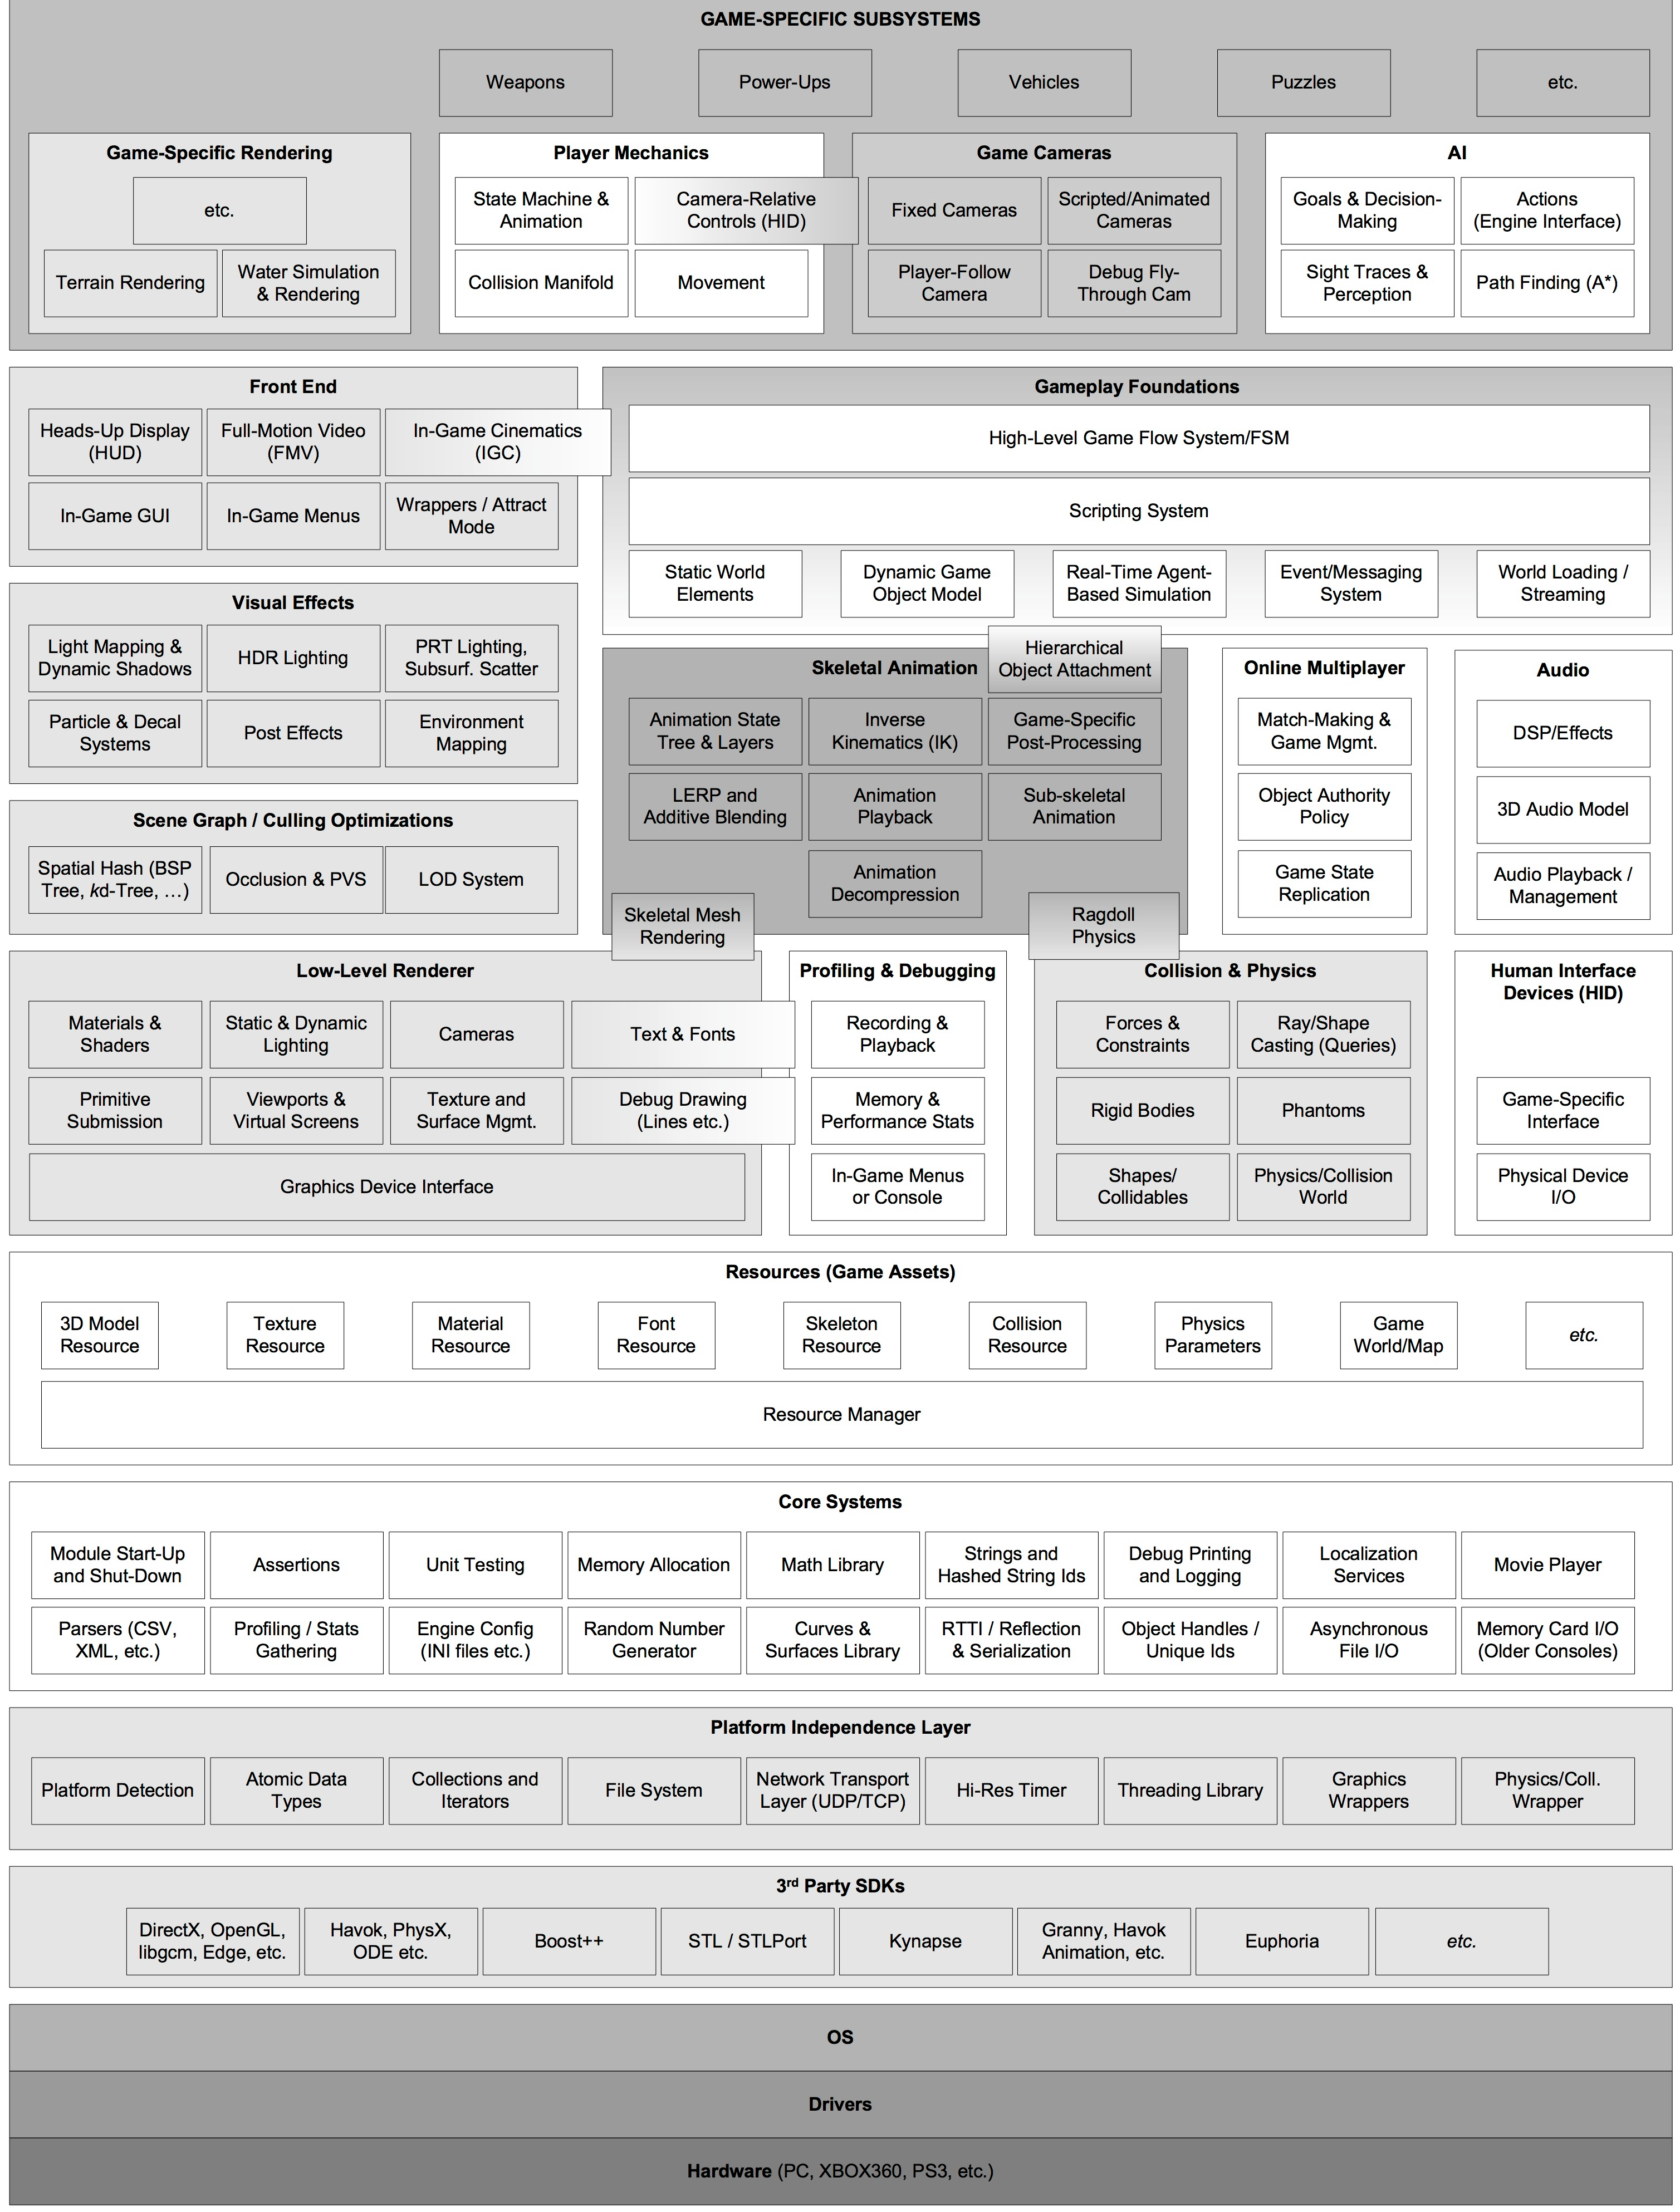
\includegraphics[width=160mm]{Images/game_engine_architecture}
		\caption{Game Engine Architecture}
		\label{fig:Game Engine Architecture}
	\end{figure}	
		
\section{Game Design}
Game design ονομάζουμε τον σχεδιασμό και την εφαρμογή τεχνικών αισθητικής στη δημιουργία ενός παιχνιδιου με σκοπό τη διευκόλυνση της αλληλεπίδρασης μεταξύ των παικτών. Οι μηχανές γραφικών χρησιμοποιούνται για σκοπούς game design.
	\subsection{MDA Model}
	To μοντελο \gls{MDA} ο σχεδιασμός παιχνιδιών χωρίζεται στα mechanics, dynamics και aesthetics.
	\cite{mda04}.
	\begin{itemize}
	\item Mechanics: τα διάφορα συστατικά ενός παιχνιδιού, στο επίπεδο αλγορίθμων και της αναπαράστασης.
	\item Dynamics: η συμπεριφορά των mechanics κατά των χρόνο εκτέλεσης, αντιδρώντας στις εισόδους και εξόδους του συστήματος με την πάροδο του χρόνου
	\item Aesthetics: οι επιθυμητές συναισθηματικές αντιδράσεις τις οποίες προκαλεί η συσκευή αναπαραγωγής όταν αλληλεπιδρά με τον παίχτη.	
	\end{itemize}

\section{Δομή μιας τυπικής ομάδας ανάπτυξης παιχνιδιών}
	Πριν από την ανάλυση της δομής της μηχανής, θα γίνει ανάλυση της δομής ομάδας η οποία θα την χρησιμοποιεί για να αναπτυχθούν στοχευμένα εργαλεία για το κάθε πρόβλημα της κάθε υπο-ομάδας.
	
	\paragraph{Μηχανικοί}	
	Οι μηχανικοί σχεδιάζουν και υλοποιούν το λογισμικό του παιχνιδιού και τα εργαλεία τα οποία χρησιμοποιούνται για την ανάπτυξή του. Οι δύο μεγάλες κατηγορίες μηχανικών είναι οι
	\begin{itemize}
		\item runtime programmers οι οποίοι ασχολούνται με τη μηχανή κται το παιχνίδι 
		\item tool programmers οι οποίοι γράφουν tools τα οποία αυτοματοποιούν και ευκολύνουν την διαδικασία ανάπτυξης.
	\end{itemize}
	Οι μηχανικοί έχουν είτε κάποια ειδικότητα, για παράδειγμα ειδικότητα στη τεχνητή νοημοσύνη, είναι είναι generalists, δηλαδή κατέχουν από όλα τα στοιχεία και μπορούν να λύσουν προβλήματα που κατά τη διάρκεια ανάπτυξης.
	
	\paragraph{Artists}
	Οι artists παράγουν όλο το οπτικοακουστικό κομμάτι του παιχνιδιού, το οποίο είναι βασικό κομμάτι για το χαρακτήρα του παιχνιδιού. Χωρίζονται στις εξής κατηγορίες
	
	\begin{itemize}
		\item Concept artists οι οποίοι σχεδιάζουν σκίτσα και πίνακες τα οποία παρέχουν στην ομάδα την εικόνα του τελικού παιχνιδιού. Παρέχουν οπτική καθοδήγηση στην ομάδα καθ' όλη τη διάρκει του κύκλου ανάπτυξης.
		\item 3D Modelers οι οποίοι είναι υπεύθυνοι για την τρισδιάστατη γεωμετρία του εικονικού κόσμου του παιχνιδιού. Απαρτίζονται από τους
		foreground modelers οι οποίοι σχεδιάζουν χαρακτήρες, οχήματα, οπλα και αντικείμενα του τρισδιάστατου κόσμου
		background modelers οι οποίοι σχεδιάζουν την στατικό περιβάλλον πχ κτήρια
		\item Texture artists οι οποίοι σχεδιάζουν τις δισδιάστατες εικόνες που καλύπτουν τα τρισδιάστατα μοντέλα
		\item Lighting artists που ορίζουν τις στατικές και δυναμικές πηγές φωτός και δουλεύουν με το χρώμα, την κατεύθυνση και την κατεύθυνση του φωτός.
		\item Animators οι οποίοι σχεδιάζουν την κίνηση των χαρακτήρων και των αντικειμένων
		\item Motion capture actors οι οποίοι παρέχουν ακατέργαστα δεδομένα κίνησης για να επεξεργαστούν οι animators και να τα ενσωματώσουν στο παιχνίδι.
		\item Sound designers οι οποίοι παράγουν τα εφέ και τη μουσική.
		\item Voice actors τους οποίους η φωνή ηχογραφείται και χρησιμοποιείται για τους χαρακτήρες στο παιχνίδι
	\end{itemize}
	
	\paragraph{Game Designers}
	Η δουλειά ενός game designer είναι να σχεδιάσει το διαδραστικό τμήμα του παιχνιδιού, το gameplay. Ασχολούνται με τον σχεδιασμό επιπέδων, την ιστορία τηις αλληλεπιδράσεις μεταξύ των χαρακτήρων στο παιχνίδι με τους στόχους, σκοπούς και κανόνες του παιχνιδιού.
	Σχεδιάζουν το κάθε επίπεδο μονδικά και αποφασίζουν για τη γεωμετρία στο περιβάλλον, πότε και που εμφανίζονται χαρακτήρες και διάφορα αντικείμενα, πως γίνονται οι μεταβάσεις μεταξύ διάφορων σκηνών κλπ.
	
	\paragraph{Producers}
	Ο ρόλος του producer διαφέρει από στούντιο σε στούντιο. Η βασική του δουλειά είναι να προγραμματίζει και να δρομολογεί τις διάφορες εργασίες και να λειτουργεί ως ο συνδετικός κρίκος μεταξύ των ατόμων που παίρνουν ηγετικές αποφάσεις και την ομάδα ανάπτυξης. Οι producers είναι χαρακτηριστικό των ΑΑΑ εταιριών, όπου υπάρχουν πολλά τμήματα και πολλοί εργαζόμενοι.	
	
		\chapter{Ο πηρύνας της Μηχανής}
	
	Ένα framework το οποίο επεκτείνεται και διακλαδώνεται σε πολλές υπο-βιβλιοθήκες, στηρίζεται στη θεμελιώση ενός framework core, του πηρύνα της βιβλιοθήκη. Το \gls{API} του πηρύνα πρέπει να είναι εύκολο στην κατανόηση, να αποτελείται από αυτοεπεξηγούμενες αφαιρέσεις, οι οποίες εκθέτουν μόνο τα απολύτος απαραίτητα, ώστε οι υποβιβλιοθήκες που χρησιμοποιούν τον πηρύνα να μην δεσμεύονται σε υλοποιήσεις, να περιορίζει σε συγκεκριμένο pipeline χρήσης για αποφυγή απρόβλεπτων συμπεριφορών και να προσφέρει δυνατότητες επεκτασιμότητας.  \cite{jaroslav08} Ο πηρύνας περιέχει υποσυστήματα τα οποία μπορούν να χρησιμοποιηθούν τη δημιουργία πολλών είδων παιχνιδιών.
		
	\section{Κύκλος ζωής πηρύνα}	
	Κάθε οντότητα από τη στιγμή της δημιουργίας της στο περιβάλλον της μηχανής μέχρι την καταστροφής της και διαγραφή της από την μνήμη, περνά από κάποια προκαθορισμένα στάδια τα οποία εκτελούνται ανάλογα με την κατάσταση του υλικού και του λογισμικού. Τα στάδια αυτά περιγράφονται στο \ref{fig:corelifecycle}
	
	\begin{itemize}
		\item Initialization εκτελείται μόνο κατά τη δημιουργία
		\item Game loop εκτελείται συνέχεια σε βρόγχο
		\item Disposing εκτελείται κατά την καταστροφή
	\end{itemize}
	
	\begin{figure}[h!]
		\centering
		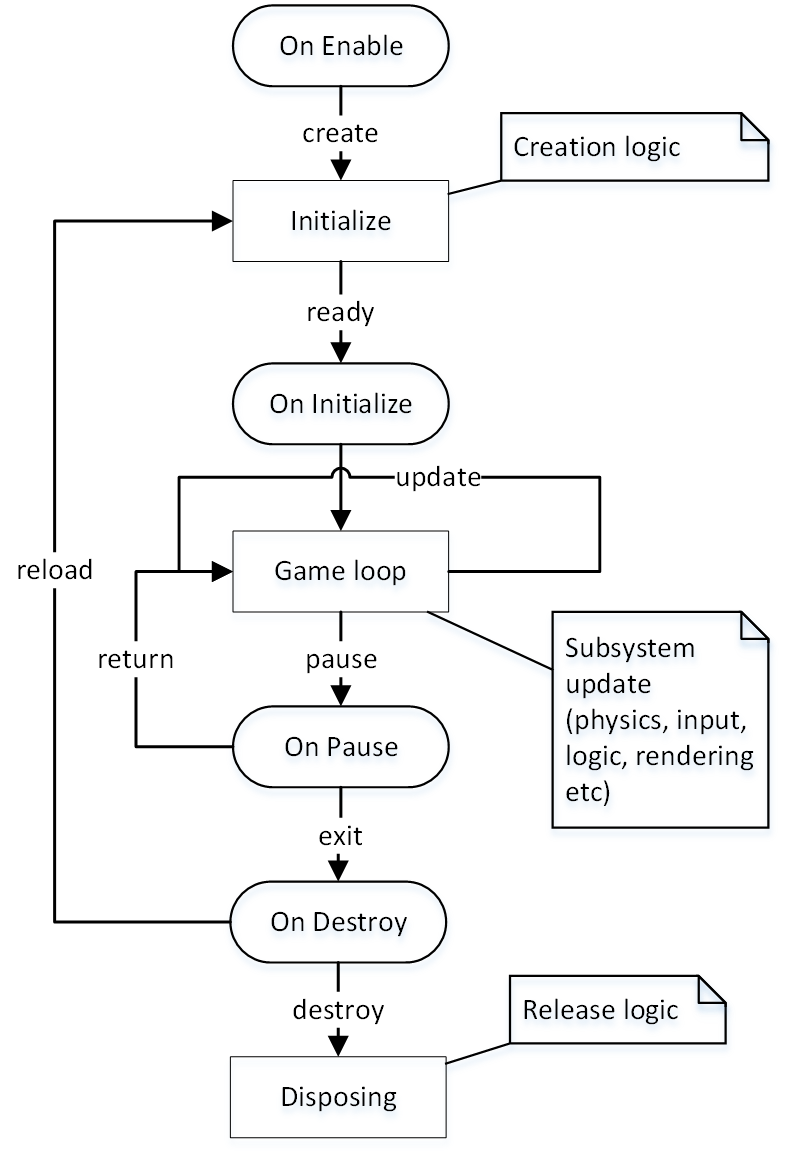
\includegraphics[width=80mm]{Images/core_lifecycle}
		\caption{Κύκλος ζωής του πυρήνα}
		\label{fig:corelifecycle}
	\end{figure}
		
	\subsection{Βρόγχος παιχνιδιού}
	Ο βρόγχος του παιχνιδιου (game loop) εγκυάται τη συνεπής ενημέρωση των υποσυστημάτων ανάλογα με το προκαθορισμένο χρονικό βήμα. Χωρίς το ανεξάρτητο σύστημα ενημέρωσης υποσυστημάτων, η ενημέρωση θα γινόταν στον κύκλο εκτέλεσης του επεξεργαστή με αποτέλεσμα την διαφορετική εμπειρία ανά επεξεργαστή και μηχάνημα. Στο game loop ενημερώνονται όλα τα υποσυστήματα \ref{fig:gameloops} 
	
	Το κάθε υποσύστημα έχει διαφορετικές απαιτήσεις για τη βέλτιστη λειτουργία. Το collision detection system μπορεί να χρειάζεται να ενημερώνεται εκατό φορές το δευτερόλεπτο, ενώ το σύστημα τεχνητής νοημοσύνης δύο φορές το δευτερόλεπτο. Η πιο συνηθισμένη τεχνική είναι να υπάρχουν δύο κύρια update loops
	\begin{itemize}
	\item το game loop στο οποίο ενημερώνονται όλα τα υποσυστήματα, physics, logic, dynamics κλπ
	\item rendering loop στο οποίο γίνονται οι κλήσεις στην κάρτα γραφικών και τρέχει στα 50-60 \gls{FPS}
	\end{itemize}
	
	Η διαφορά του χρόνου μεταξύ των ενημερώσεων πρέπει να είναι εγγυημένη για παράδειγμα σε μια μηχανή στην οποία το rendering loop τρέχει στα 60 \gls{FPS} υπάρχει η συχνότητα ενημέρωσης
	\begin{equation}
	 F = 1/T =>  F = 1000ms/60 => F = 16ms. 
	\end{equation}Για να μπορεί να εγγυάται το σύστημα αυτή την αναλογία, πρέπει να μετράει τη διαφορά χρόνου μεταξύ κάθε κλήσης, να εκτελεί τον κώδικα στο συγκεκριμένο loop και για τον υπόλοιπο χρόνο το thread να κοιμάται.
	
	\begin{figure}[h!]
		\centering
		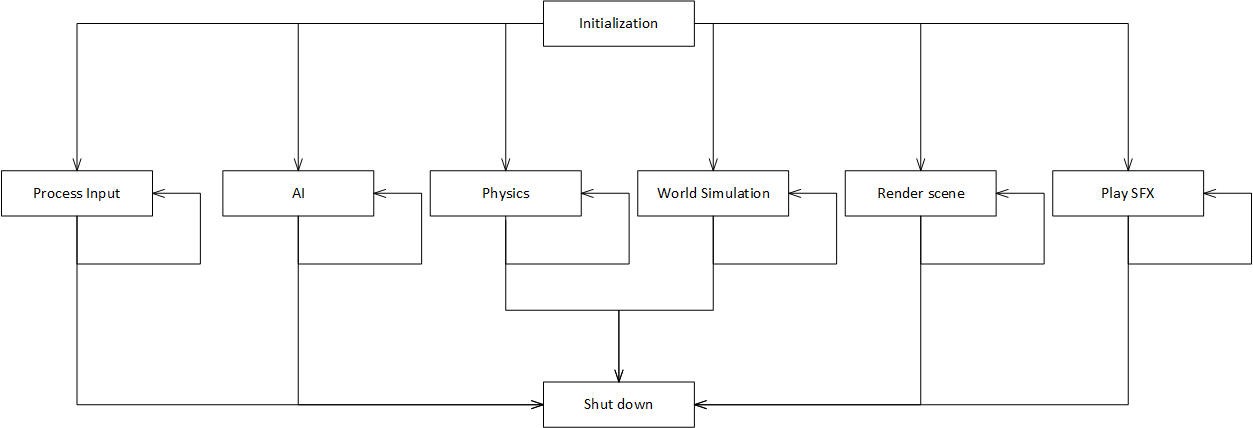
\includegraphics[width=160mm]{Images/gameloops_update}
		\caption{Game loop}
		\label{fig:gameloops}
	\end{figure}
		
	\paragraph{Χρόνος}
	Στα συστήματα πραγματικού χρόνου, η έννοια της διάρκειας και του χρόνου πρέπει να χειρίζεται απομονωμένος. Ο χρόνος του παιχνιδιού  είναι ανεξάρτητος από τον πραγματικό χρόνο. Η ενημερώση και η λογική των συστημάτων γίνεται με βάση τη διαφορά χρόνου μεταξύ ενημερώσεων. Με αυτή την στρατηγική, η εμπειρία δεν διαφοροποιείται με λιγότερα \gls{FPS} και ένα animation το οποίο γίνεται render σε πραγματικό χρόνο, μπορεί να παίξει αντίστροφα ή με διπλάσια ταχύτητα, αν το χρονοδιάγραμμα στο οποίο ανταποκρίνεται, χειρίζεται τον χρόνο διαφορετικά.
	Όλα τα συστήματα ενημερώνονται γραμμικά συναρτήσει μιας αφαίρεσης η οποία περιλαμβάνει τη διαφορά χρόνου.
	\subsection{Υποσυστήματα}
	Το κάθε υποσύστημα δημιουργείται ενημερώνεται και καταστρέφεται μέσα στο γενικό κύκλο ζωής του πηρύνα. Το κάθε υποσύστημα έχει εσωτερικά το δικό του κύκλο ζωής και κύκλο ενημέρωσης ο οποίος λειτουργεί μέσα στην έκταση του εξωτερικού κύκλου ζωής.
	
	\subsection{Τεχνικές Ενημέρωσης Υποσυστημάτων}
	Τα υποσυστήματα με κάποιο τρόπο πρέπει να ενημερώνονται και να επικοινωνούν μεταξύ τους ή να στέλνουν μηνύματα όταν συμβεί κάποιο γεγονός. Υπάρχουν διάφορές τεχνικές ενημέρωσης υποσυστημάτων.
	\begin{itemize}
	\item Message Pumps: τα υποσυστήματα στέλνουν μηνύματα σε ένα message bus και τα συστήματα ενημερώνονται όταν εξυπηρετείται το μήνυμα. Παραμένουν άεργα εφόσον δεν υπάρχει μήνυμα προς εξυπηρέτηση.
	\item Call-back driven: τα υποσυστήματα παρέχουν call-back λειτουργικότητα. Δηλαδή τη δυνατότητα να θέσεις τι κώδικας θα εκτελεστεί κατά κάποιο συμβάν. Ένα συμβάν μπορεί να είναι η σύγκρουση μεταξύ δύο αντικειμένων. Ο χρήστης μπορεί να πει ότι όταν συμβεί σύγκρουση μεταξύ του παίχτη και του εχθρού, ο παίχτης θα χάσει ζωή.
	\end{itemize}
		
	\section{Διαχείριση οθονών}
	Σε ένα τυπικό χρόνο εκτέλεσης ενός παιχνιδιού, το παιχνίδι περνά από διάφορες καταστάσεις. Οι καταστάσεις αυτές μπορεί να είναι η προσωρινή παύση, ένα μενού ρυθμίσεων ένα \gls{GUI} επιλογών το οποίο επικαλύπτει το τρέχον παιχνίδι ή απoδίδεται στον ίδιο render buffer. Το παιχνίδι χωρίζεται σε σκηνές, σε επίπεδα και σε χάρτες οι οποίες έχουν ξεχωριστό τρόπο απόδοσης στην οθόνη. Μία σκηνή μπορεί να αποδίδεται από διάφορες υποσκηνές οι οποίες δίνουν την ψευδαίσθηση του βάθους στο φόντο. Η σειρά απόδοσης των σκηνών πρέπει να είναι ρυθμιζόμενη και ελεγχόμενη. Η κάθε σκηνή μπορεί να παρομοιαστεί ως μια οθόνη.

	\subsection{Απαιτήσεις}
	Ο χρήστης του συστήματος έχει πλήρη έλεγχο της κάθε οθόνης-σκηνής και προσαρμόζει τη λογική και την απόδοση ανάλογα. Το κεντρικό σύστημα διαχείρισης προσφέρει τη δυνατότητα προετοιμασίας οθονών, αναζήτησης μέσω κλειδιών, αυτόματη διαχείριση και εναλλαγή και εξατομίκευση τους. Για τη διατήρηση της συνοχής κατά την εναλλαγή οθόνων, προσφέρεται η δυνατότητα εξατομίκευσης της απόδοσης κατά τις μεταβάσεις. Μια τυπική χρήση του συστήματος παρουσίαζεται στ διάγραμμα ακολουθίας \ref{fig:screensystem_sequence}.

	\begin{figure}[h!]
		\centering
		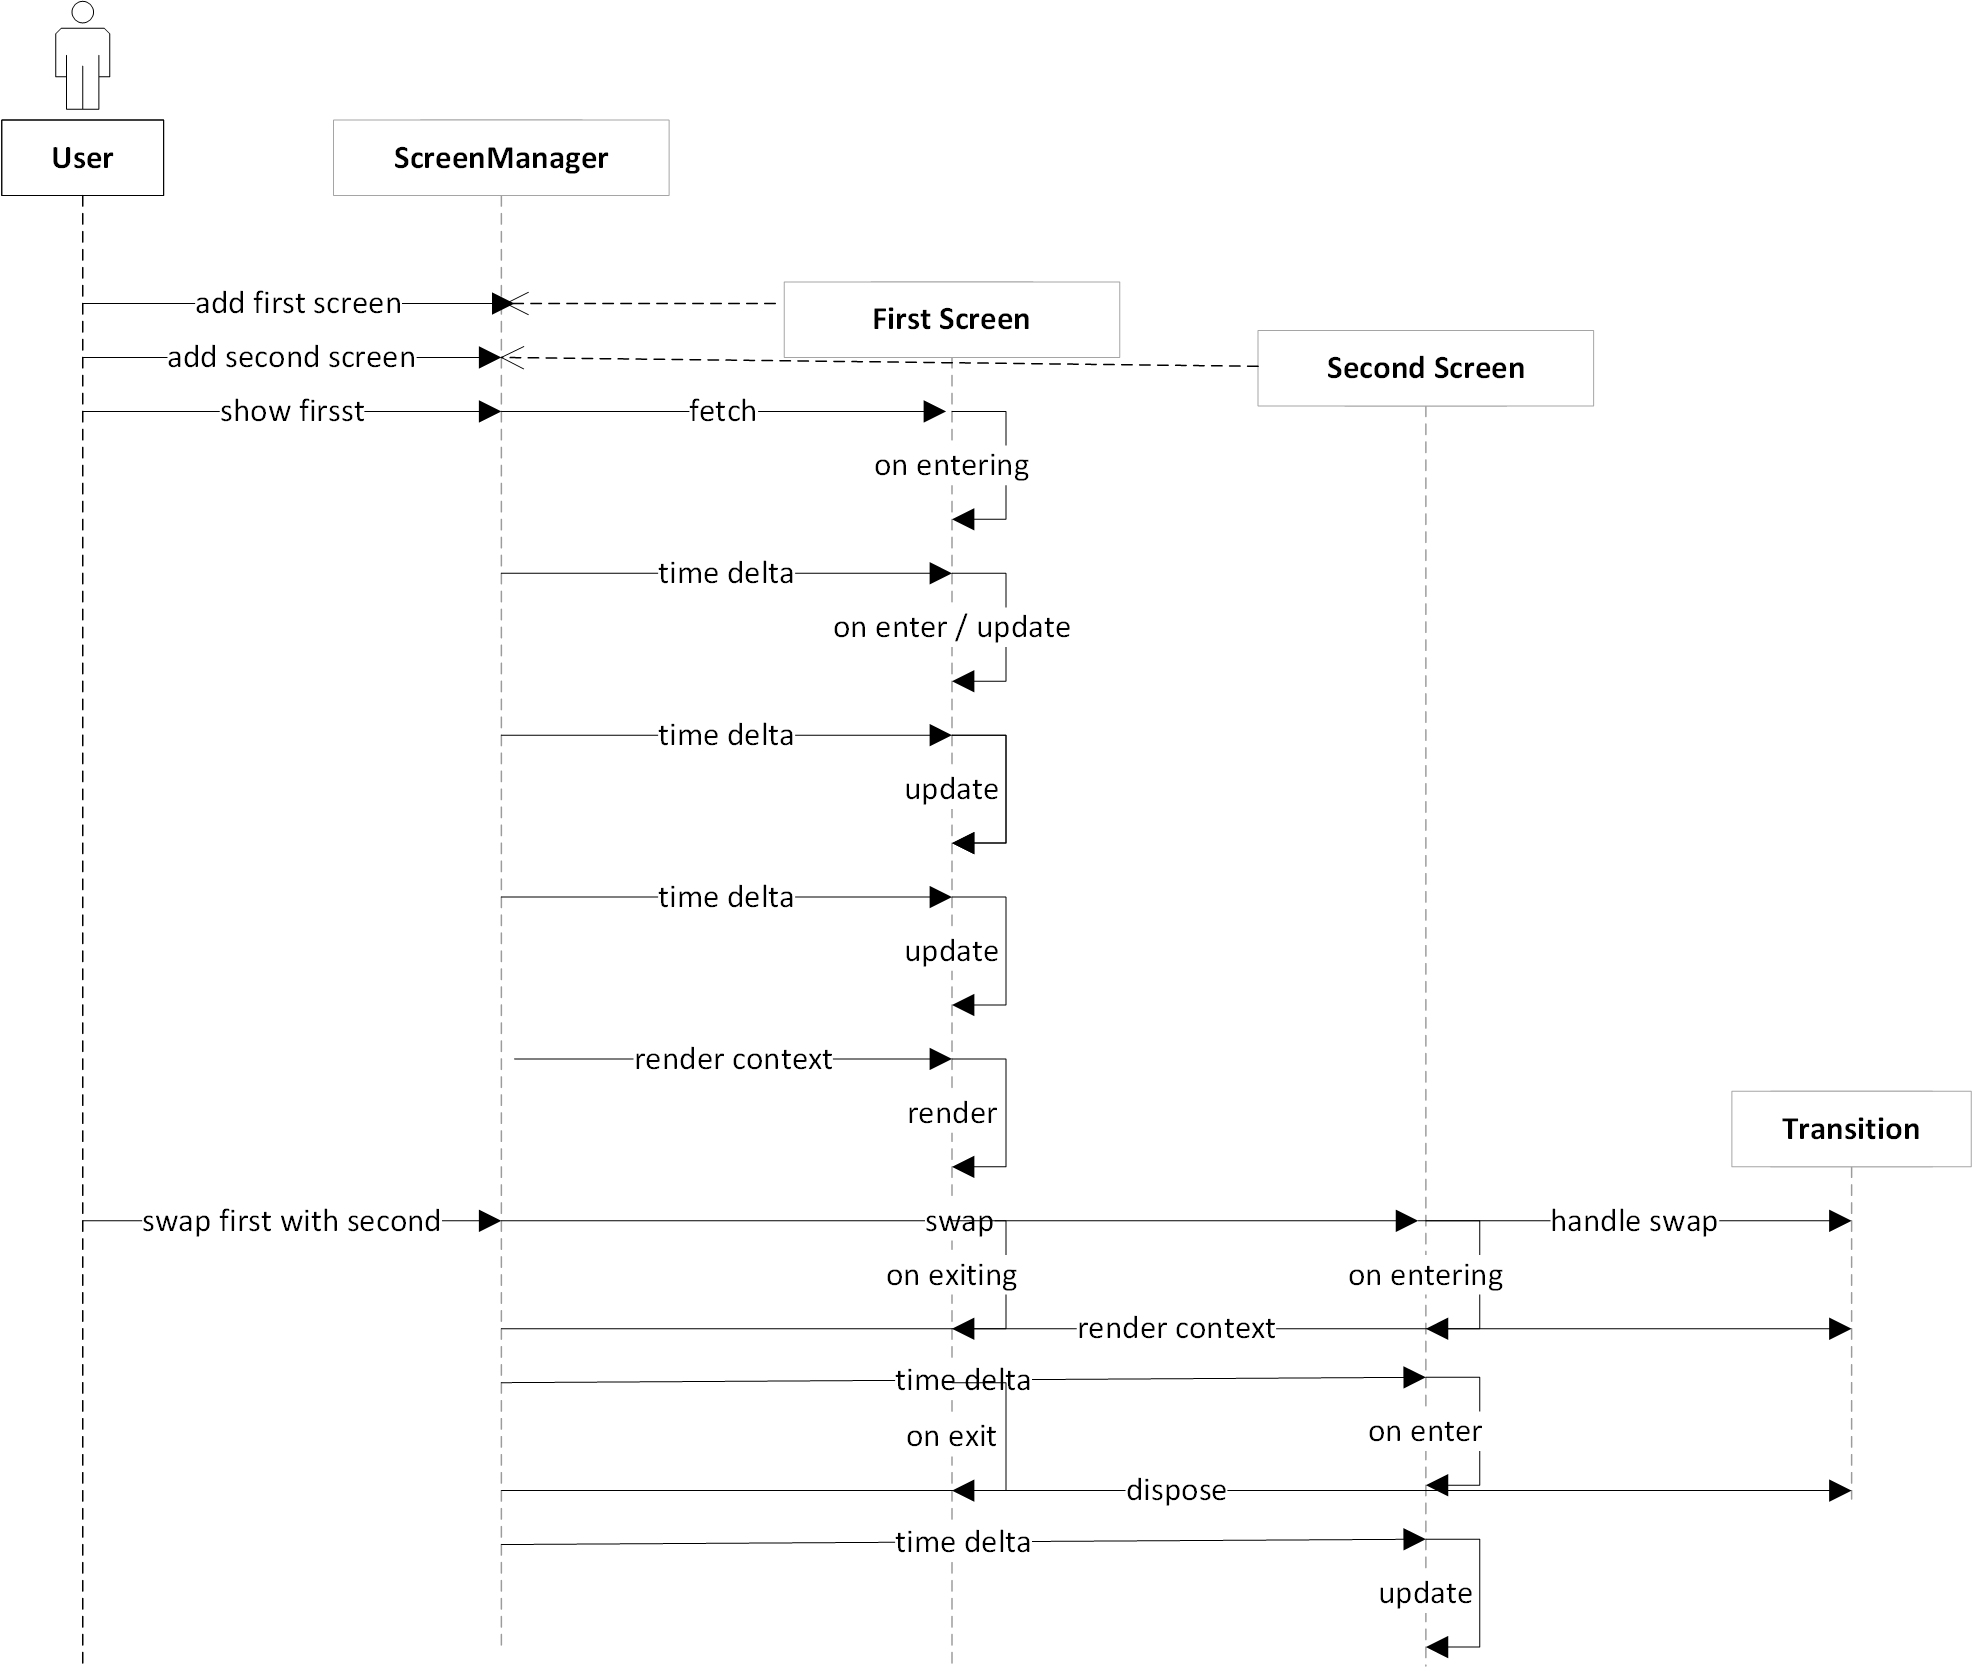
\includegraphics[width=165mm]{Images/screensystem_sequence}
		\caption{screensystem sequence}
		\label{fig:screensystem_sequence}
	\end{figure}	
	
	\subsection{Συστατικά του συστήματος}		
	\paragraph{Κεντρικό σύστημα διαχείρισης}
	Οι λειτουργίες του συστήματος.
	\begin{itemize}
	\item Απόδοση και ενημέρωσης 1-N σκηνών με δυναμικά εναλλασσόμενη σειρά στο πλαίσιο του κύκλου ζωής του πηρύνα.
	\item Προετοιμασία των οθονών και δυνατότητα εύρεσης χρησιμοποιώντας κλειδιά.
	\item Εύκολη προβολή, απόκριψη, εναλλαγή οθονών χρησιμοποιώντας κλειδιά.
	\item Δυνατότητα εξατομίκευσης της απόδοσης κατά τις διάφορες μεταβάσεις των σκηνών.
	\end{itemize}

	\paragraph{Screen host}
	\begin{itemize}
		\item Παραμετροποίηση συμβάντων κατά τις αλλαγές κατάστασης
		\item Προσαρμοσμένη λογική και απόδοση 
		\item Εντολές αλλαγής κατάστασης
		\item Εξατομίκευση απόδοσης κατά την εναλλαγή κατάστασης
	\end{itemize}
	
	\paragraph{Εναλλαγή οθονών}
	Η εξατομίκευση και παραμετροποίηση της εναλλαγής οθονών λαμβάνει μέρος μέσα στο γενικό πλαίσιο απόδοσης οθονών. Ο εξατομικευτής αναλαμβανει την απόδοση του screen buffer στον οποίο αποδόθηκε η οθόνη, την κατάσταση στην οποία βρίσκεται η οθόνη, την κατεύθυνση και το ποσοστό εξέλιξης της εναλλαγής. 
			
	\lstset
	{
		style=sharpc, 
		caption={Transition Delegate}
	}
	\begin{lstlisting}	
delegate void TransitionRenderAction(ScreenState state, float progress, RenderTarget2D renderTarget, SpriteBatch batch);
	\end{lstlisting}
	
	\newpage
	\subsection{Αρχιτεκτονική}
Η αρχιτεκτονική του υποσυστήματος παρουσιάζεται στο UML διάγραμμα \ref{fig:core_screensystem}.
	\begin{figure}[h!]	
		\centering
		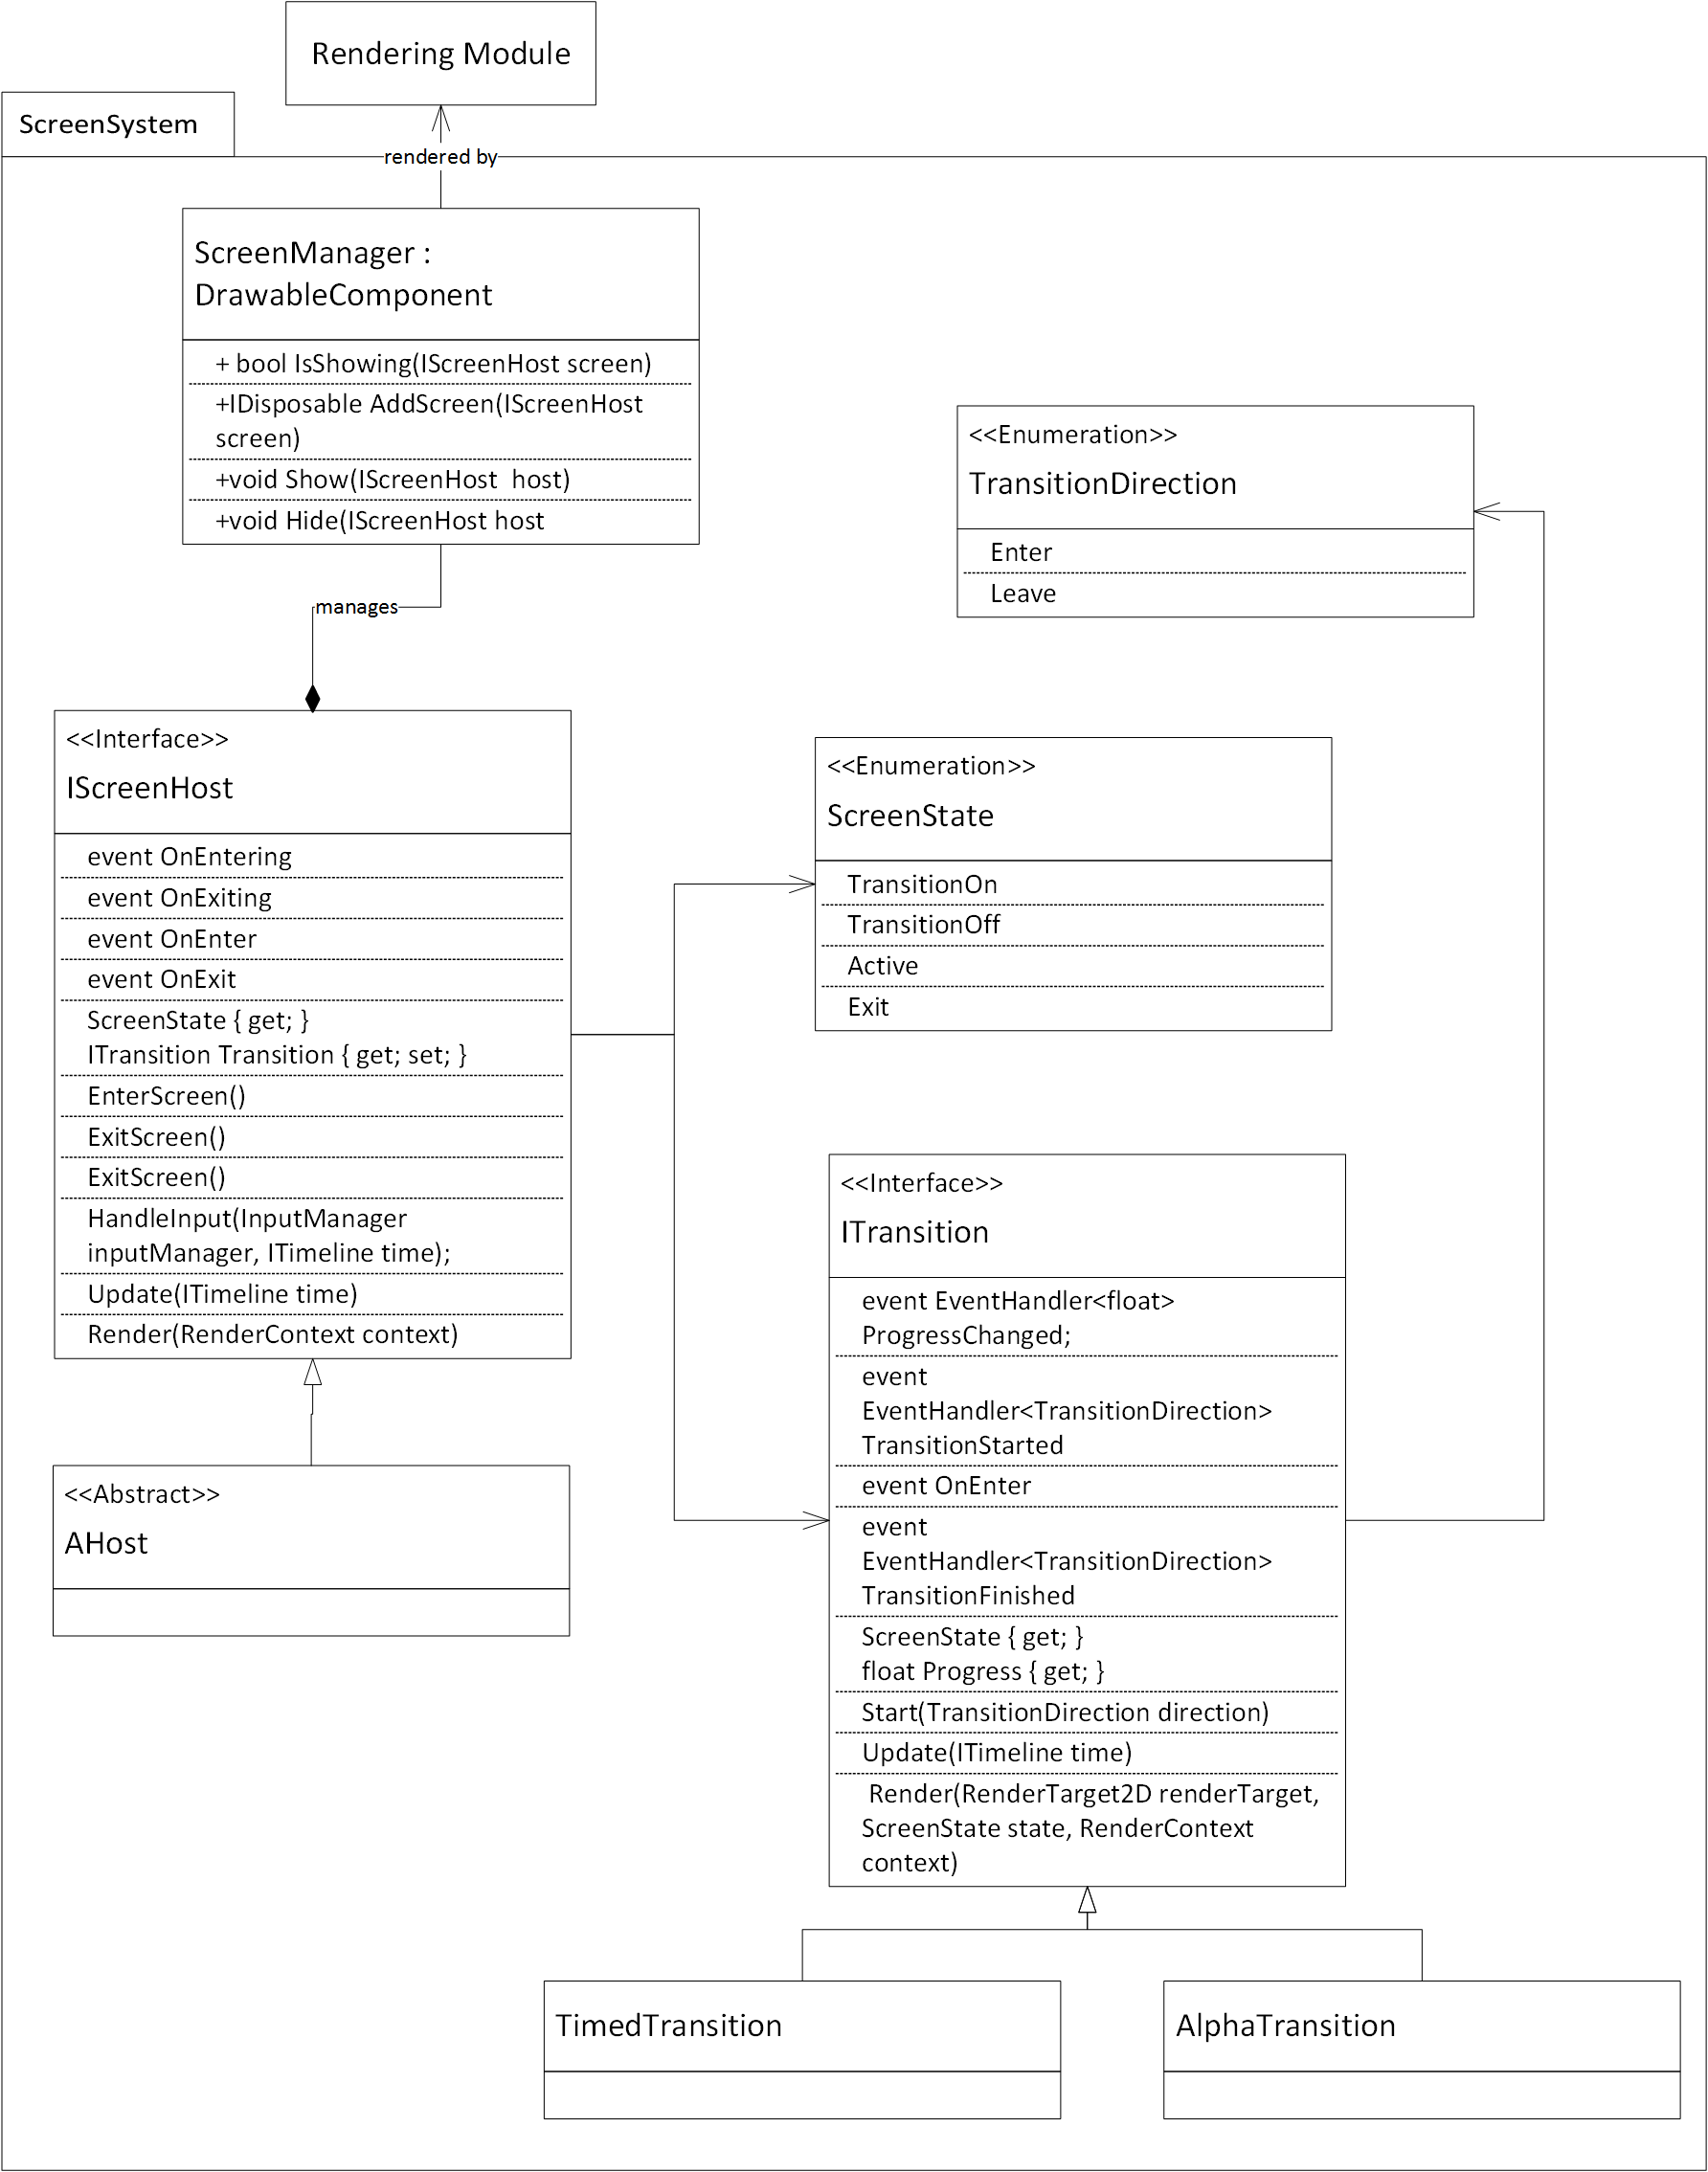
\includegraphics[width=160mm]{Images/core_screensystem}
		\caption{Screen System UML}
		\label{fig:core_screensystem}
	\end{figure}		
	
	\subsection{Παράδειγματα χρήσης API}

	\lstset
	{
		style=sharpc, 
		caption={Transition Delegate}
	}
	\begin{lstlisting}
screenHost
.AddScreen(
	"FirstScreen",
	() => new MyFirstScreen());
		
screenHost["FirstScreen"]
.Show()
.Transition(
	Transition.WithTime(
         TimeSpan.FromSeconds(0.5),
         (state, progress, target, context) =>
         context.Batch.Draw(target, 
         (float)Math.Pow(progress - 1.0f, 2) * context.ScreenWidth, 
         Color.White * progress
    )
);
     
screenHost["FirstScreen"]
.Hide();   
	\end{lstlisting}
	
	\section{Σύστημα εισόδων}
	\subsection{Human Interface devices}
	Η μηχανή πρέπει να είναι σε θέση να διαβάζει, να επεξεργάζεται και να χρησιμοποιεί συσκευές ανθρώπινης διεπαφής. Η διαδικασία ανάγνωσης χωρίζεται στις παρακάτω κατηγορίες:
	\begin{itemize}
	\item Polling: η κατάσταση κάποιον συσκευών (κυρίως της παλιάς σχολής) διαβάζεται ρωτώντας τη συσκευή για την κατάστασή της περιοδικά. Αυτό καταλήγει σε πλεονασμό γιατί ρωτάει πολλές φορές χωρίς να παίρνει απάντηση και με μικρή καθυστέρηση γιατί η αλλαγή κατάστασης μπορεί να γίνει μεταξύ ερωτήσεων.
	\item Interrupts (διακοπές): Οι συσκευές στέλνουν δεδομένα μόνο όταν αλλάξει η κατάσταση με κάποιο τρόπο. Ο χρήστης μπορεί γράψει κώδικα και να τον εγγράψει με τρόπο ώστε να εκτελείται μόνο όταν συμβεί κάποια αλλαγή κατάστασης.
	\end{itemize}
	
	\subsection{Τύποι εισόδου}
	
	\begin{itemize}	
	\item Digital Buttons: τα ψηφιακά κουμπιά έχουν δύο καταστάσεις: pressed / not pressed
	\item Analog axes and buttons: τα αναλογικά επιστρέφουν εύρος τιμών: το βαθμό της πίεσης της σκανδάλης ή τη θέση του μοχλού στο δισδιάστατο άξονα. 
	\item Relative Axes: οι αναφορικοί άξονες επιστρέφουν τιμές σε σχέση με το τελευταίο σημείο στο οποίο έγινε κάποια αλλαγή πχ το ποντίκι επιστρέφει τη διαφορά θέσης σε σχέση με το τελευταίο σημείο στο οποίο μετακινήθηκε.
	\item Accelerators: Ανιχνεύουν τρισδιάστατες επιταχύνσεις.
	\item Sensor bars: Αισθητήρες όπως οι κάμερες.
	\item Touch / gestures: Σε οθόνες αφής όπως στις οθόνες στα έξυπνα τηλέφωνα.
	\end{itemize}
	
	\subsection{Απαιτήσεις υποσυστήματος}
	Η οντότητα θέλει να εκτελέσει κώδικα προσανατολισμένο κατά συμβάν εισόδου από συσκευή ανθρώπινης διεπαφής. Ο κώδικας αυτός εκτελείται αντίστοιχα για keyboard-mouse και για gamepad. O χρήστης μπορεί να αλλάξει συσκευή διεπαφής ενώ βρίσκεται σε τρέχον παιχνίδι. Η βιβλιοθήκη δεν πρέπει να στηρίζεται σε κανένα υλικό ή συσκευή. Επίσης θέλει τη δυνατότητα να ακυρώνει συμβάντα.
		
	\subsection{Observers-listeners}
	Το κάθε υποσύστημα διαχείρισης συσκευών ανθρώπινων διεπαφών αποτελείται από τον διαχειριστή για παράδειγμα τον MouseListener ή Keyboard listener, το οποίο χρησιμοποιεί τις βιβλιοθήκες του τρέχον λειτουργικού για την επιστολή συμβάντων των διεπαφών. Ανάλογα με την πλατφόρμα στην οποία έγινε compile δημιουργούνται οι αντίστοιχοι listeners μέσω του abstract factory.
	Ο χρήστης μπορεί να προσκολήσει κώδικα ο οποίος να εκτελείται ανά συμβαν π.χ. στη μετακίνηση του ποντικιού.Οι listeners κατά την εισαγωγή τους, επιστρέφουν ένα αντικείμενο το οποίο μπορεί να χρησιμοποιηθεί για την κατάργησή τους. Οι listeners ανάλογα με τις συνθήκες επιστολής, όπως το δέλτα του χρόνου επιστολής συμβάντος διπλού click ειναι 200ms, αποστέλλουν τα συμβάντα στoυς καταχωρημένους εκτελεστές. Το κεντρικό σύστημα διαχείρισης εισόδου ενημερώνει όλες τις συνδεδεμένες συσκευές εισόδου. 
	Ο εκτελέσιμος κώδικας μπορεί να γραφτεί μια φορά, ανεξαρτήτως συμβάντος, και να προσκοληθεί στο initialization του lifecycle σε υποσυστήματα διεπαφών. Επίσης με τη χρήση των active binders, μπορεί να γίνει απενεργοποίηση των listeners π.χ. όταν είναι ανοιχτό το menu επιλογών, οι o ActiveBinder του παιχνιδιού είναι απενεργοποιημένος, με αποτέλεσμα τα συμβάτα τα οποία είναι προσκολλημένα στον InputManager να μην εκτελούνται. Στο uml διάγραμμα \ref{fig:core_input} παρουσιάζεται η αρχιτεκτονική του συστήματος τον listeners.
	
	
	\begin{figure}[h!]
		\centering
		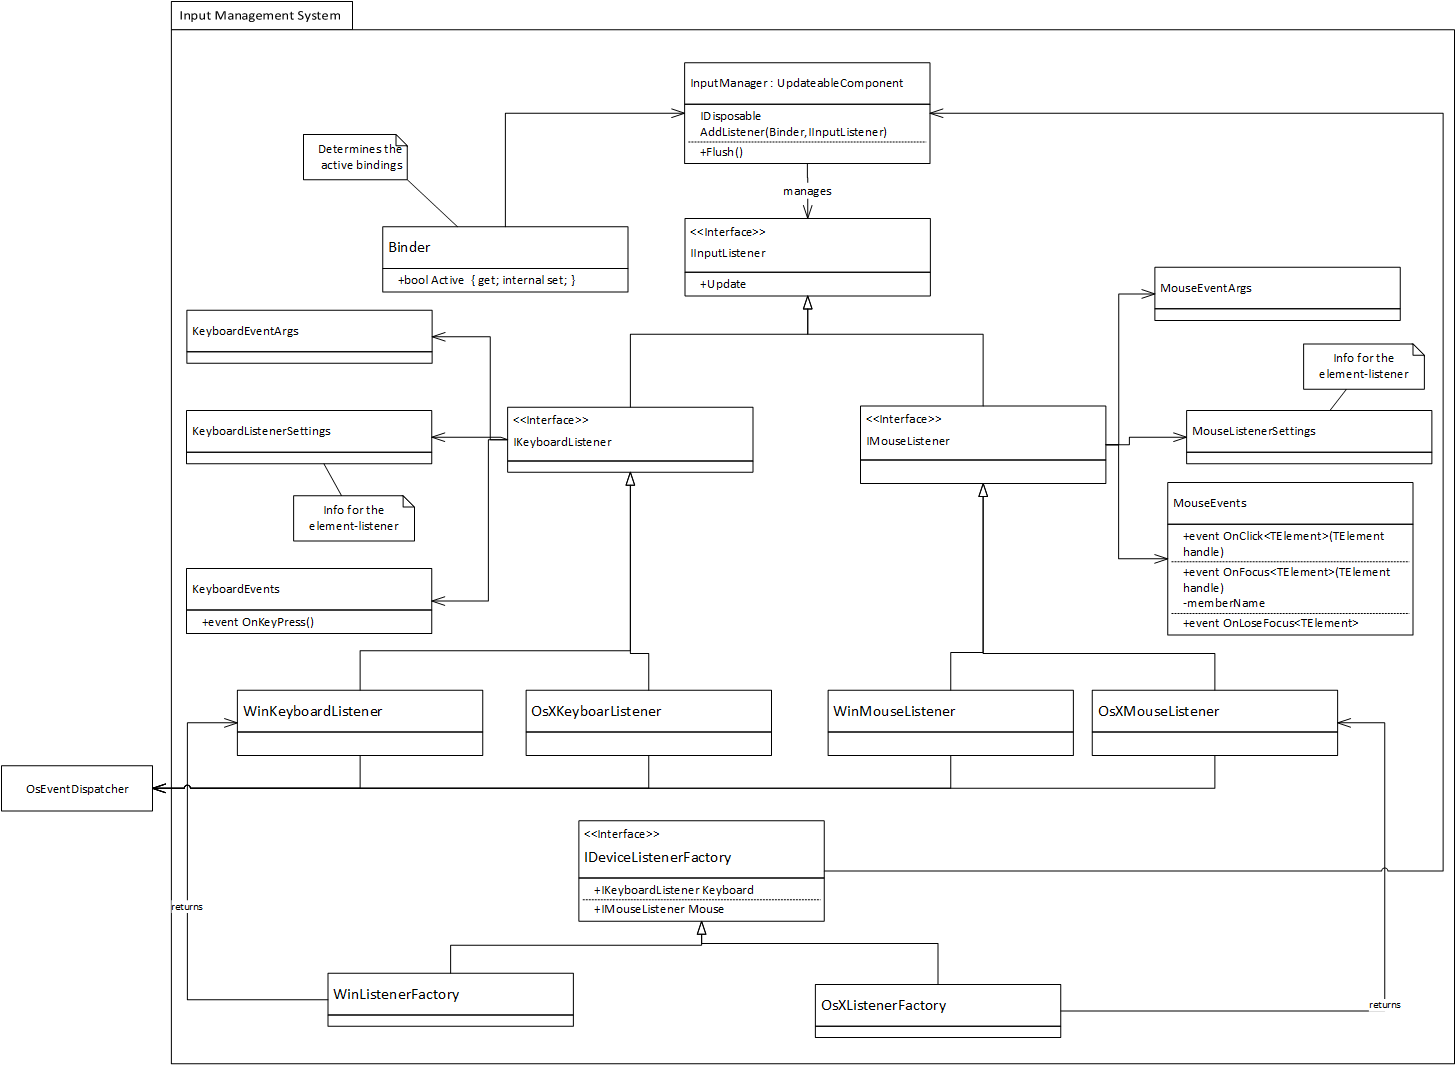
\includegraphics[width=165mm]{Images/core_input}
		\caption{Input System UML}
		\label{fig:core_input}
	\end{figure}
		
	\newpage
	\paragraph{API}
	Στο παράδειγμα \ref{cs:listeners} παρουσιάζεται η δημιουργία και καταχώρηση των listeners. 
	\lstset
	{		
		style=sharpc, 
		caption={Παράδειγμα καταχώρησης listeners}
	}
	\label{cs:listeners}
	\begin{lstlisting}
inputManager.AddListener(
ingameBinder,
factory => factory.GamepadListener
{
	Settings = MouseSettings
		    .DoubleClickDelta(Timespan.FromSeconds(0.2))
			.DragDelta(Timespan.FromSeconds(0.2)),
	Events   = MouseEvents
	        .OnLeftClick(sender,args) => this.Shoot())
	        .OnLeftDoubleClick(sender,args) => this.Roll())      	
});

inputManager.AddListener(
ingameBinder,
factory => factory.GamepadListener
{
	Settings = GamepadSettings.Default,
	Events   = GamepadEvents
			.OnXButtonPress(sender,args) => this.Shoot())
			.OnYButtonPress(sender,args) => this.Roll())      	
});
\end{lstlisting}

\section{Φυσική και συγκρούσεις}
Η φυσική στα παιχνίδια έχουν ως βάση τα μαθηματικά. Η ανάλυση του συστήματος της φυσικής επικεντρώνεται σε μοντελοποίηση υψηλού επιπέδου. Η υλοποίησή τους βασίζεται υλοποίηση μαθηματικών λειτουργιών γεωμετρίας, γραμμικής άλγεβρας και κινηματικής.

\subsection{Τα παιχνίδια ως soft real-time simulations}
Οι επιστήμονες αποκαλούν τα παιχνίδια soft real-time interative agent-based computer simulations.
Στα περισσότερα παιχνίδια ένα υποσύστημα του πραγματικού κόσμου μοντελοποιείται μαθηματικά, ώστε να μπορεί να αναπαραχθεί και να χειριστεί από τον υπολογιστή. 
Ενα agent-based simulation είναι μια προσομοίωση η οποία περιγράφει πως αλληλεπιδρούν τα διάφορα αντικείμενα και χαρακτήρες μέσα στον κόσμο.
Όλα τα αλληλεπιδραστηκά παιχνίδια είναι temporal simulations δηλαδή ο το μοντέλο του εικονικού κόσμου είναι δυναμικό, αλλάζει με την πάροδο του χρόνου, με βάση τα διάφορα συμβάντα και την εξέλιξη της ιστορίας.
Όλα simulations και η επικοινωνία του παιχνιδιού με τον χρήστη γίνεται σε πραγματικό χρόνο (interactive real-time simulations. 

Στον πυρήνα όλων τον συστημάτων πραγματικού χρόνου υπάρχει το at least 24 fps deadline δηλαδή για να δημιουργείται η ψευδαίσθηση της κίνησης, η οθόνη θα πρέπει να ανανεώνεται τουλάχιστον 24 φορές το δευτερόλεπτο. Φυσικά υπάρχουν και άλλα είδη deadlines. Για να θεωρείται η προσομοίωση φυσικής σταθερή, πρέπει να ενημερώνεται τουλάχιστον 120 φορές το δευτερόλεπτο, ο μηχανισμός τεχνητής νοημοσύνης θα πρέπει να καλείται τουλάχιστον κάθε δευτερόλεπτο, οι audio buffers 60 φορές το δευτερόλεπτο για να αποτρέπονται δυσλειτουργίες του συστήματος διαχείρησης ήχου.

Ένα soft real time system είναι ένα σύστημα στο οποίο χαμένες ενημερώσεις δεν είναι καταστροφικές.
Τα μαθηματικά μοντέλα τα οποία απαρτίζουν το σύστημα μπορεί να είναι είτε αριθμητικά είτε αναλυτικά. Τα αριθμητικά μοντέλα μπορούν να αξιολογηθούν για κάθε τιμή της ανεξάρτητης μεταβλητής ενώ οι τιμές του αναλυτικού μοντέλου καθορίζονται διακρίτα κατά τη διάρκεια της προσομείωσης και είναι πιο συχνά γιατί η επόμενη κατάσταση της προσομείωσης καθορίζεται από την εισαγωγή δεδομένων σε πραγματικό χρόνο από το χρήστη. \cite{realtime_collision04}

\subsection{Βασικές έννοιες φυσικής του συστήματος}
Οι οντότητες της φύσικης έχουν τις παρακάτω ιδιότητες για τη προσομοίωσή τους στο υποσύστημα φυσικής.

\begin{itemize}
\item Mass: Η μάζα στη φυσική συνδέεται με δύο έννοιες, την αδράνεια της μεταφορικής κίνησης και τη βαρύτητα. Η μάζα είναι μια ορισμένη ποσότητα η οποία χρησιμοποιείται για την περιγραφή ενός συστήματος.

\item Density:  Η πυκνότητα εκφράζει τη μάζα του υλικου που περιέχεται σε μία μονάδα όγκου. 

\item Force: Σε ότι αφορά τα ελεύθερα σώματα, η δύναμη είναι γενικά η αιτία μεταβολής της κινητικής τους κατάστασης, δηλαδή αυτή που τα επιταχύνει ή τα επιβραδύνει. Αυτό ισχύει και για την περιστροφή τους, που μπορεί να επιταχυνθεί ή να επιβραδυνθεί. Για σώματα που δεν είναι ελεύθερα να κινηθούν με όλους τους τρόπους, αυτά δηλαδή που είτε είναι αναρτημένα κάπου και μπορούν να κινηθούν μόνο γύρω από σημείο ή άξονα ή σε προκαθορισμένη τροχιά, καθώς και σε όσα εφαρμόζονται δυνάμεις τριβής ή γενικά αντιδράσεις στήριξης.

\item Torque: Ροπή δυνάμεως ως προς σημείο είναι το διανυσματικό φυσικό μέγεθος που έχει μέτρο ίσο προς το γινόμενο της δύναμης επί την (κάθετη) απόσταση της δύναμης από το σημείο. Κατά όμοιο τρόπο ροπή δυνάμεως ως προς άξονα είναι το διανυσματικό μέγεθος που έχει ως μέτρο το γινόμενο της δύναμης επί την (κάθετη) απόσταση της δύναμης από τον άξονα, και φορέα τον άξονα.

\item Impulse: Η ώθηση είναι φυσικό μέγεθος που ισοδυναμεί με την μεταβολή της ορμής ενός σώματος στο οποίο εφαρμόζεται μία δύναμη για κάποιο χρονικό διάστημα. Ισούται με το γινόμενο της δύναμης που ασκείται στο σώμα επί τον συνολικό χρόνο εφαρμογής της

\item Restitution: Το law of restitution δηλαδή ανάκτυση με βάση το κέρδος. Η υποχρέωση της οντότητας να αποζημιώσει από τα κέρδη τη για κάποιο γεγονός. 

\item Damping: Η απόσβεση, η επιρροή εντός η κατά ενός συστήματος ταλάντωσης που έχει ως αποτέλεσμα τη μείωση, τον περιορισμό η την πρόληψη των ταλαντώσεών του. Σε φυσικά συστήματα , απόσβεση παράγεται με διαδικασίες που διαχέουν την ενέργεια που αποθηκεύεται στο ταλάντωση.
\end{itemize}

\subsection{Οντότητες του συστήματος}
\begin{itemize}
\item Shape
Ένα αντικείμενο το οποίο αντιπροσωπεύει ένα γεωμετρικό σχήμα όπως κύκλο, πολύγωνο κλπ
\item World
Η συλλογή των bodies, fixtures και constraints και η λογική της αλληλεπίδρασής τους.
\item World Solver
Ο solver αναλύει την προσομοίωση και εκτελείται ανεξάρτητα από το χρόνο εκτέλεσης του προγράμματος.
\item Fixture 
To fixture δένει ένα body με ένα shape και προσθέτει επιπλέον ιδιότητες όπως πυκνότητα, τριβή και αποκατάσταση. Το fixture εντάσσει ένα σχήμα στο σύστημα συγκρούσεων ώστε να αλληλεπιδρά με τα υπόλοιπα σχήματα στον κόσμο.
\item Body 
To body περιέχει της πληροφορίες ένος αντικειμένου του οποίου δεν βλέπεις ούτε συγκρούεσαι. Έχουν τις παρακάτω ιδιότητες
	\begin{itemize}
		\item mass To βάρος
		\item velocity η ταχύτητα και η κατεύθυνση της κίνησης υπό μορφή διανύσματος.
		\item rotation inertia πόσος κόπος χρειάζεται για να ξεκίνησει η περιστροφή ή η κίνηση
		\item angular velocity πόσο γρήγορα και σε ποια κατεύθυνση περιστρέφεται
		\item που βρίσκεται στο σύστημα καρτεσιανών συντεταγμένων
		\item angle υπό ποια γωνία βρίσκεται
	\end{itemize}
Οι τύποι των bodies είναι:
	\begin{itemize}
		\item Static
		Στατικά στο σύστημα συντεταγμένων. Δεν ανταποκρίνεται σε εξωτερικές δυνάμεις.
		\item Dynamic
		Είναι μέρος του συστήματος συγκρούσεων. Ανταποκρίνεται σε εξωτερικές δυνάμεις και κανονικά σε όλες τα μέρη της προσωμοίωσης.
		\item Kinematic 
		Κινείται ανάλογα με το προκαθορισμένο script ταχύτητας. Δεν ανταποκρίνεται σε εξωτερικές δυνάμεις.
	\end{itemize}
\item Constraint
Περιορισμός κατά την προσωμοίωση του body.
\item Joint 
Το joint συνδέει δύο ή περισσότερα bodies μεταξύ τους.
\item Joint Motor
Ο οδηγός της κίνησης των συνδεδεμένων με joint bodies. 
\item Joint Limit
Περιορίζει το εύρος κίνησης του joint motor.
\end{itemize}

\subsection{Αρχιτεκτονική}
Η σχέσης μεταξύ των οντοτήτων παρουσιάζονται στο διάγραμμα \ref{fig:physics_abstract}
	\begin{figure}[h!]
		\centering
		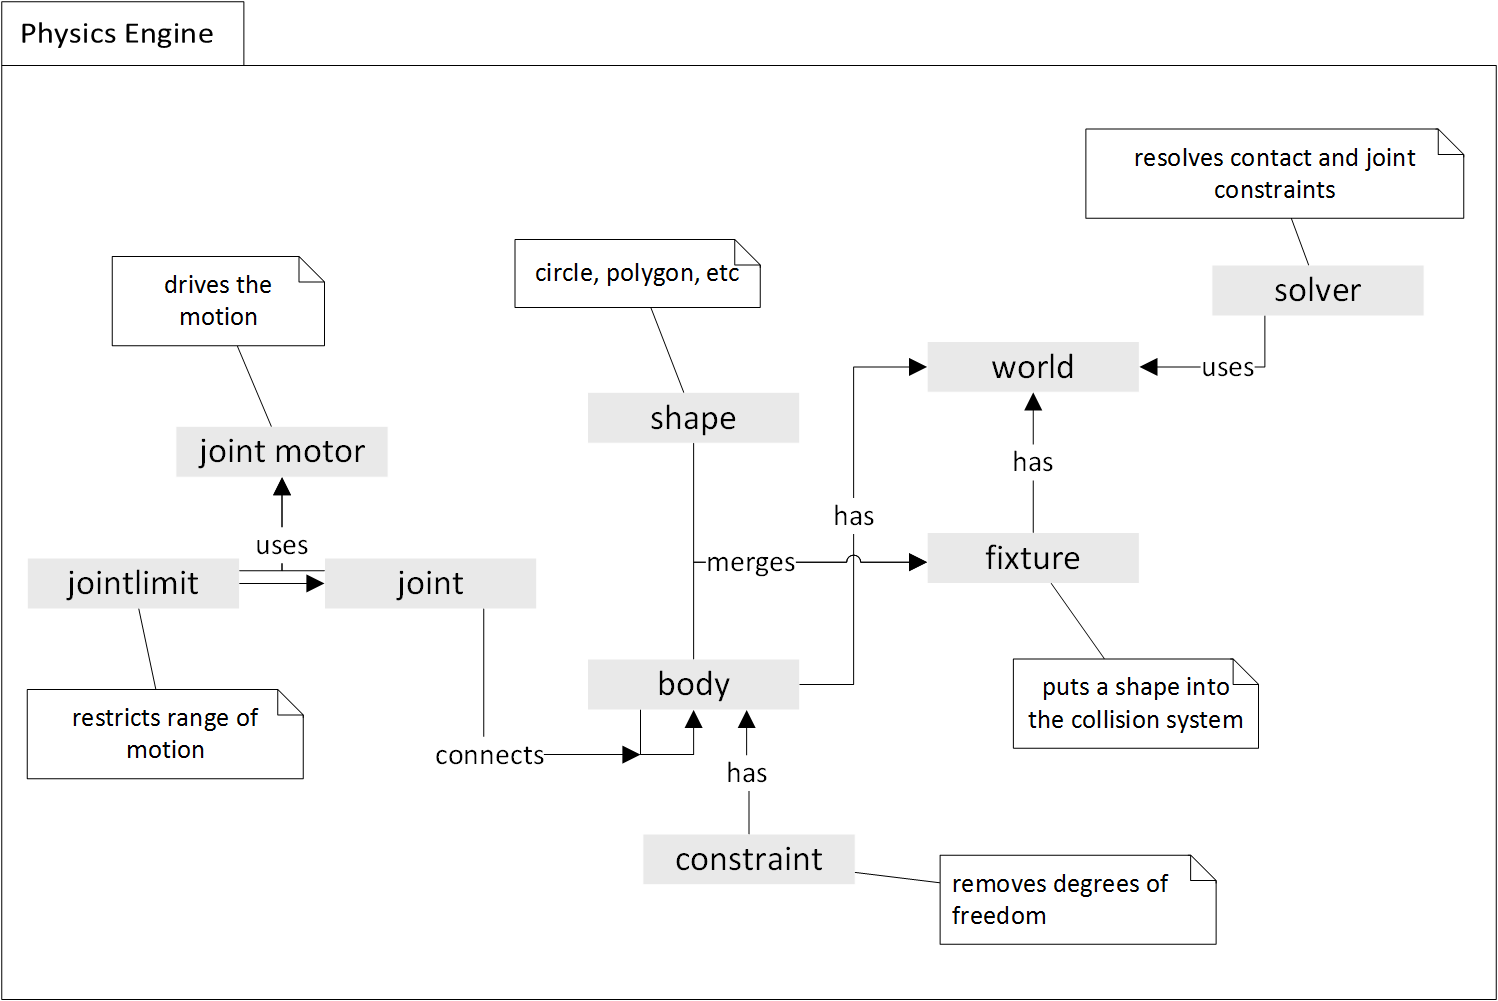
\includegraphics[width=165mm]{Images/physics_overview}
		\caption{Physics System}
		\label{fig:physics_abstract}
	\end{figure}
	
\section{Διεπαφή χρήστη}
Η επικοινωνία του χρήστη με τη μηχανή γίνεται συνήθως με human interface devcices. Η επικοινωνία αυτή αντί να περιορίζεται σε ένα απλό input signal, μπορεί να γίνει εύκολα, αυτονόητα, αποτελεσματικα και φιλικά προς το χρήστη. Το User interface (διεπαφή χρήστη) ονομάζουμε το σύνολο γραφικών στοιχείων, τα οποία εμφανίζονται στην οθόνη κάποιας ψηφιακής συσκευής (π.χ. Η/Υ) και χρησιμοποιούνται για την αλληλεπίδραση του χρήστη με τη συσκευή αυτή. Παρέχει μέσω γραφικών ενδείξεις και εργαλεία προκειμένου ο χρήστης να φέρει εις πέρας κάποιες επιθυμητές λειτουργίες.

\subsection{Απαιτήσεις}
Κατά το σχεδιασμό ενώς παιχνιδίου συχνά δημιουργείται η ανάγκη για διεπαφή χρήστη. Η δομή του UI, το στυλ της απόδοσης (χρώμα, textures, fonts κλπ),η απόδοσης (rendering) και η συμπεριφορά και ο εκτελέσιμος κώδικας κατά τα συμβάντα της διεπαφής πρέπει να είναι αποσυνδεδεμένα έτσι ώστε να μην επηρεάζει το ένα το άλλο. Επίσης χρησιμεύει όταν το UI προορίζεται για διάφορες αναλύσεις και \Gls{DPI}. Μια καλή στρατηγική σστην κατανόηση και επίλυση προβλημάτων είναι η εύρεση παρόμοιων και σχετικών προβλημάτων. Στο σχεδιασμό ιστοσελίδων η HTML χρησιμοποιείται και τη δομή της σελίδας, το CSS για το στυλ και η Javascript για τη συμπεριφορά.

\subsection{Δομή στη μνήμη}	
Όταν ζητηθεί από τον περιηγητή να φορτώσει μια ιστοσελίδα στη μνήμη από κάποιον web server, αναλύει το html αρχειο και οργανώνει τα στοιχεία σε δομή δέντρου \gls{B-Tree}. Λόγω της οργάνωση σε δέντρο, δημιουργούνται σχέσεις μεταξύ των στοιχείων.

	\begin{figure}[h!]
		\centering
		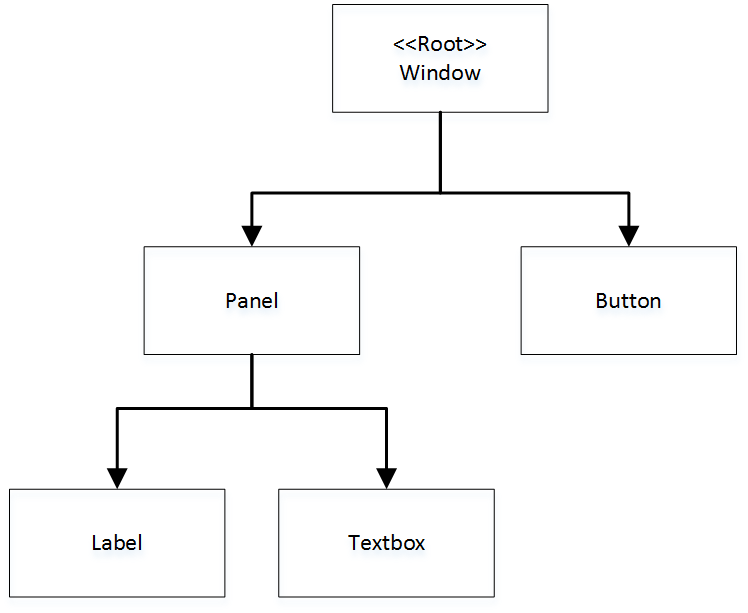
\includegraphics[width=90mm]{Images/ui_btree}
		\caption{UI B-Tree}
		\label{fig:ui_b-tree}
	\end{figure}
	
Στο παράδειγμα \ref{fig:ui_b-tree}  το window είναι το root του δέντρου. Το window έχει δύο παιδιά, ένα panel και ένα button. Το button έχει με και αυτό δύο παιδιά: ένα textbox και ένα label. Τα button, textbox και label είναι leafs του δέντρου, το panel είναι node, και το panel και button siblings.

\paragraph{Γιατί b-tree;}
Η οργάνωση σε b-tree έχει τα παρακάτω πλεονεκτήματα.
\begin{itemize}
	\item Ευκολία κατά την απόδοση στην οθόνη. Λόγω της συγκεκριμένης δομή, τα στοιχεία μπορούν να στοιχιθούν και να αποδοθούν ανάλογα με τη σχέση τους με συγγενικά στοιχεία. Καθώς διαβαίνεται το δεντρο, το κάθε στοιχείο αποδίδεται μέσα στο πλαίσιο του πατέρα του και σε πιο πάνω επίπεδο, ούτως ώστε να δημιουργείται η ψευδαίσθηση του βάθους, δηλαδή ότι το στοιχείο παιδί βρίσκεται "πάνω" άπο τον πατέρα.
	\item Καλύτερη απόδοση στο rendering. Όταν κάποιος κόμβος δεν διατέμνεται με το πλάισιο του παράθυρου, δεν απόδίδεται στην οθόνη και το traversing του δέντρου σταματά.
	\item Αποσαφήνιση σειράς συμβάντον. Κατά τα συμβάντα στο UI, ένα πλαίσιο μπορεί να καλύπτει περισσότερα από ένα συμβάντα. Ένα στοιχείο έχει τεμνόμενα πλαίσια όταν οποίο βρίσκεται μέσα σε ένα άλλο στοιχείο. To συμβάν γίνεται στο στοιχείο το οποίο βρίσκεται τελευταίο στην ιεραρχία.
	\item Προχωρημένη και γρήγορη επιλογή στοιχείων. Η επιλογή των στοιχείων γίνεται με προχωρημένα κριτήρια, όπως τη σχέση ενός στοιχείου με συγγενικά στοιχεία στη δομή, και σε λογαριθμηκό χρόνο.
	
Στο UML διάγραμμα \ref{fig:ui_structure} παρουσιάζεται το υποσύστημα το οποίο είναι υπεύθυνο για το κτίσημο του UI στη μνήμη.
\end{itemize}
	\begin{figure}[h!]
		\centering
		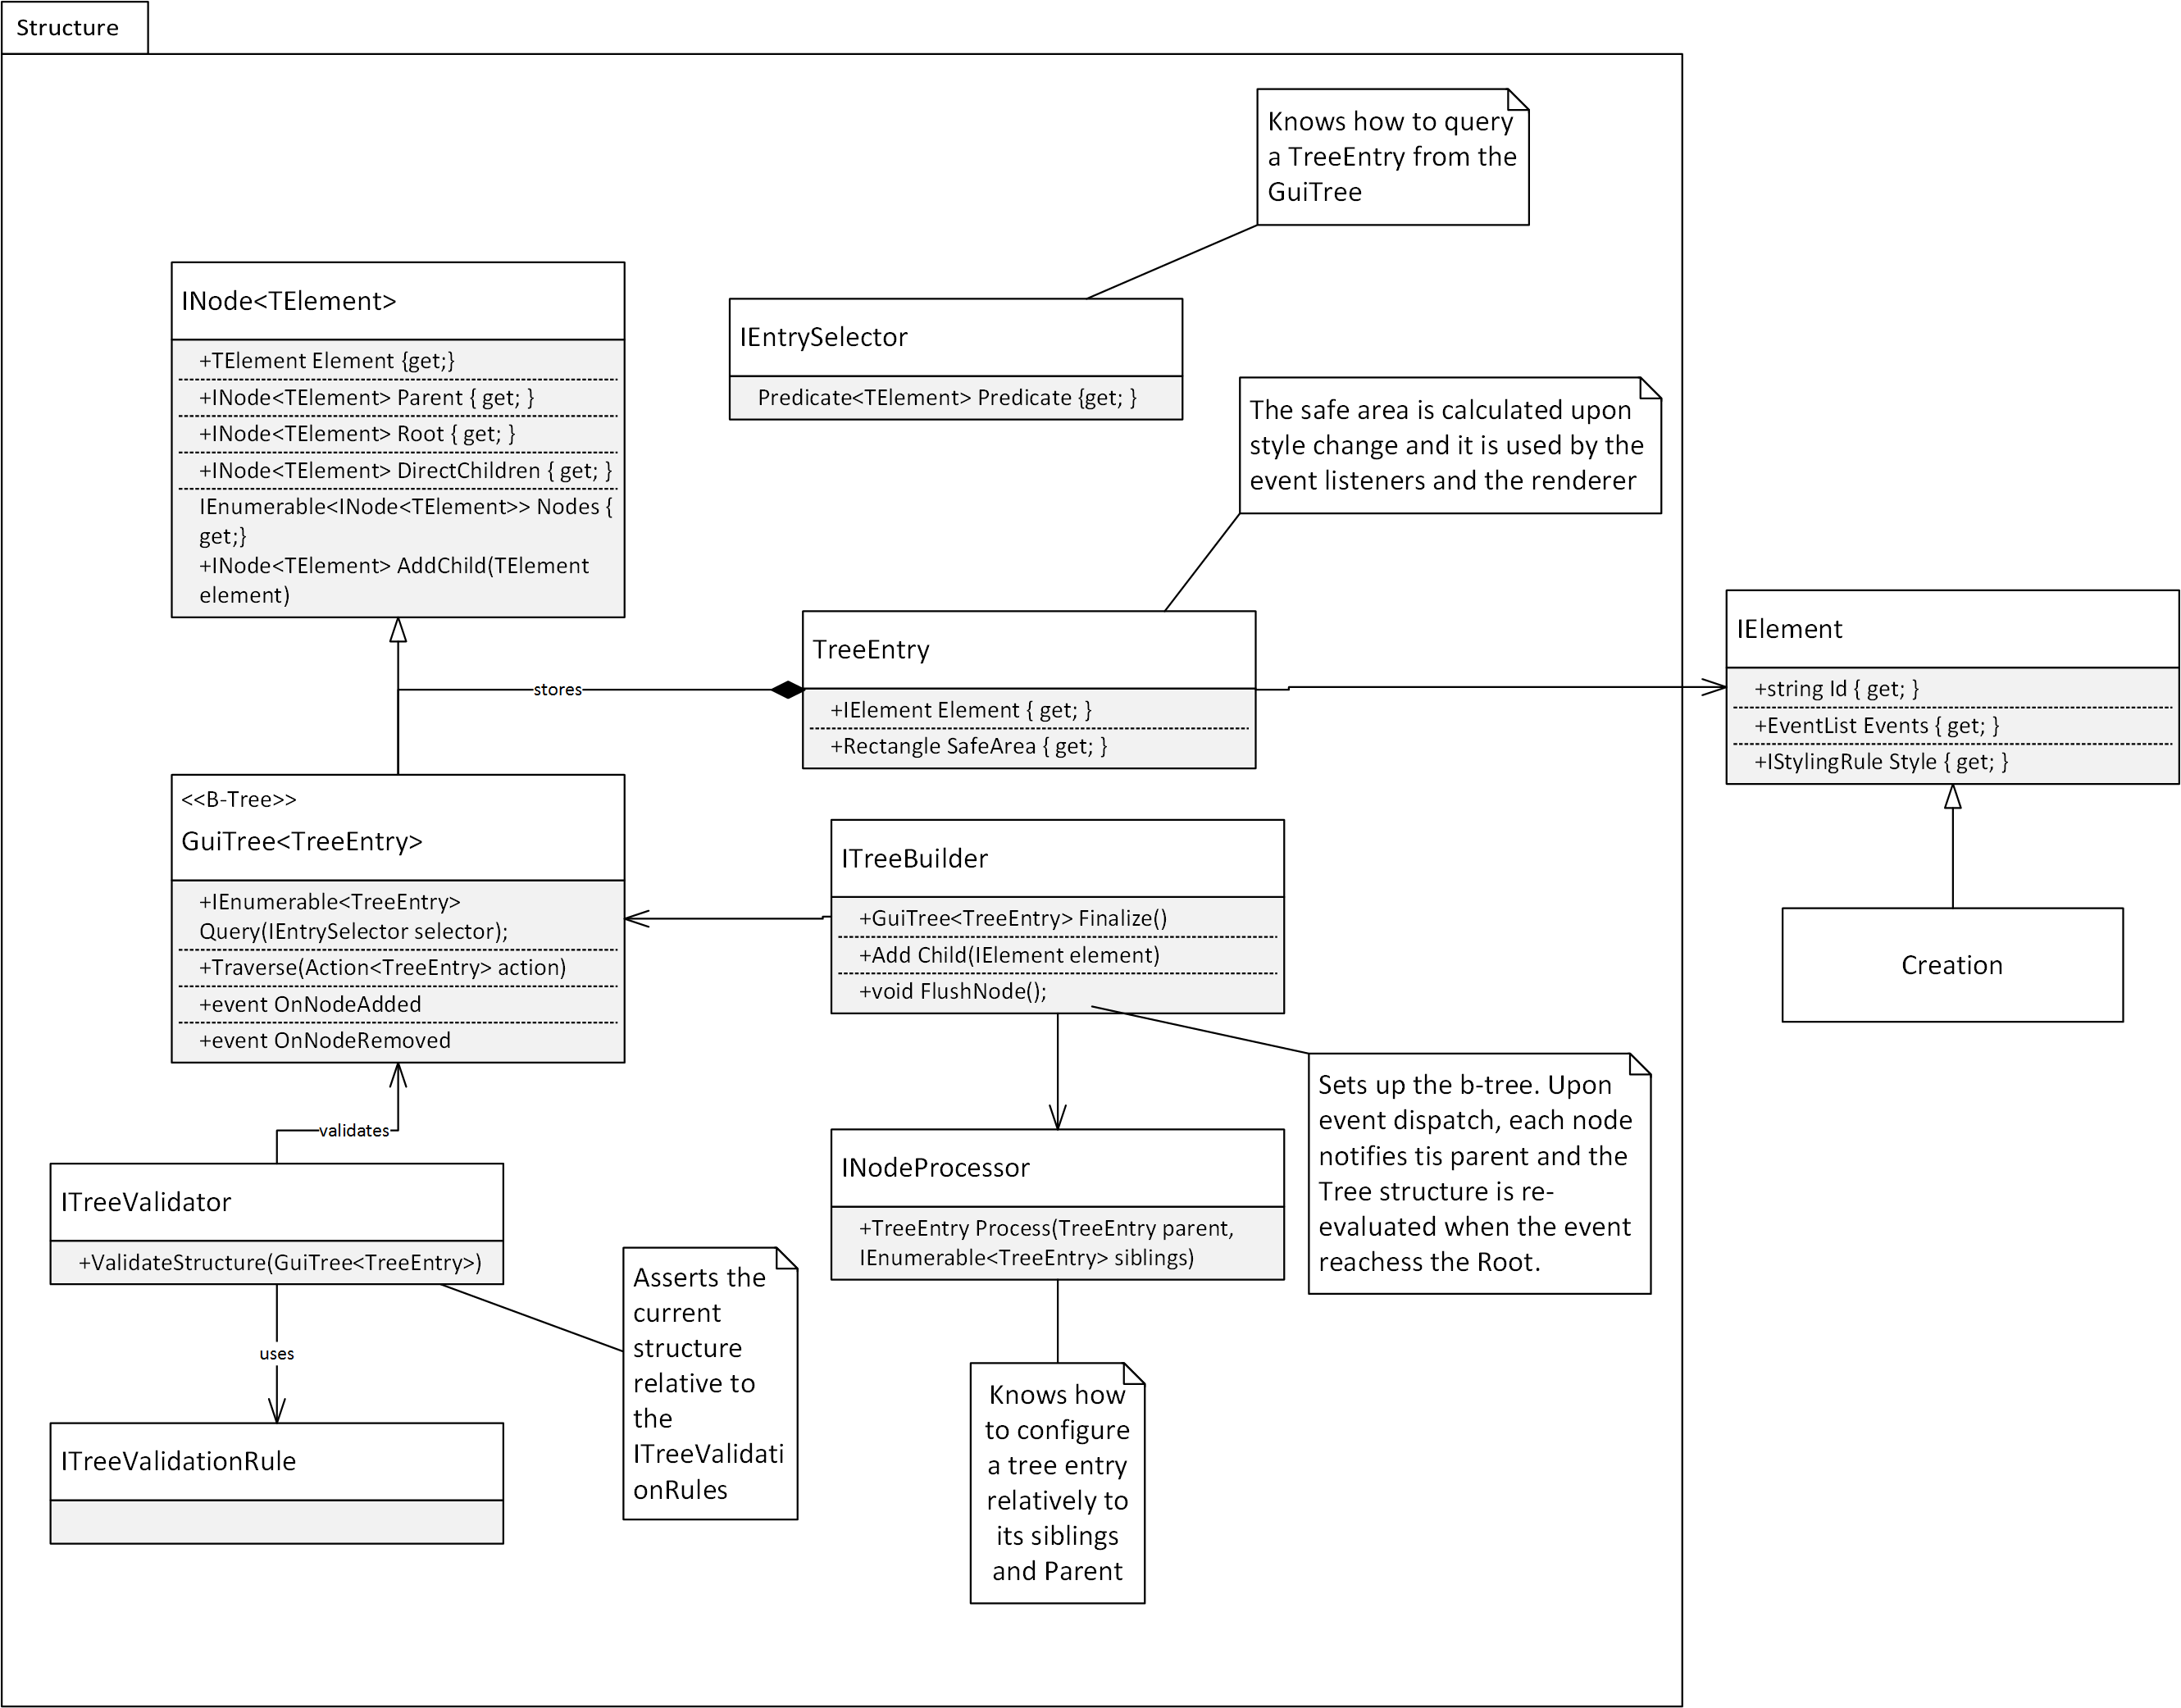
\includegraphics[width=165mm]{Images/gui_structure}
		\caption{UI Structure}
		\label{fig:ui_structure}
	\end{figure}

\subsection{Το σύστημα}	
Το σύστημα ανθρώπινης διεπαφής χωρίζεται στα παρακάτω υποσυστήματα
	\begin{itemize}
		\item Οργάνωσης δομής, το οποίο κτίζει και αποθηκεύει την ιεραρχία τον στοιχείων στη μνήμη
		\item Style definition το οποίο επαυξάνει την απόδοση με animations, textures κλπ
		\item Factory μέσα από το οποίο ο χρήστης δημιουργεί στοιχεία. Στο υποσύστημα αυτό, όπως και το input listener factory είναι χρησιμοποιεί abstract factory για δημιουργεία στοιχείων ανεξαρτήτου πλατφόρμας, και fluent builder για τη δημιουργία στοιχείων με φιλικό στον χρήστη \gls{API}.
		\item Επεκτίνει και χρησιμοποιεί με το input system για να συνδέει συμβάντα με στοιχεία
		\item Επεκτίνει και χρησιμοποιεί το rendering module για να αποδίδει το δεντρο στην οθόνη.
	\end{itemize}
	
Οι σχέσεις μεταξύ των υποσυστημάτων του συστήματος UI παρουσιάζονται στο UML διάγραμμα \ref{fig:ui_system}.
	\begin{figure}[h!]
		\centering
		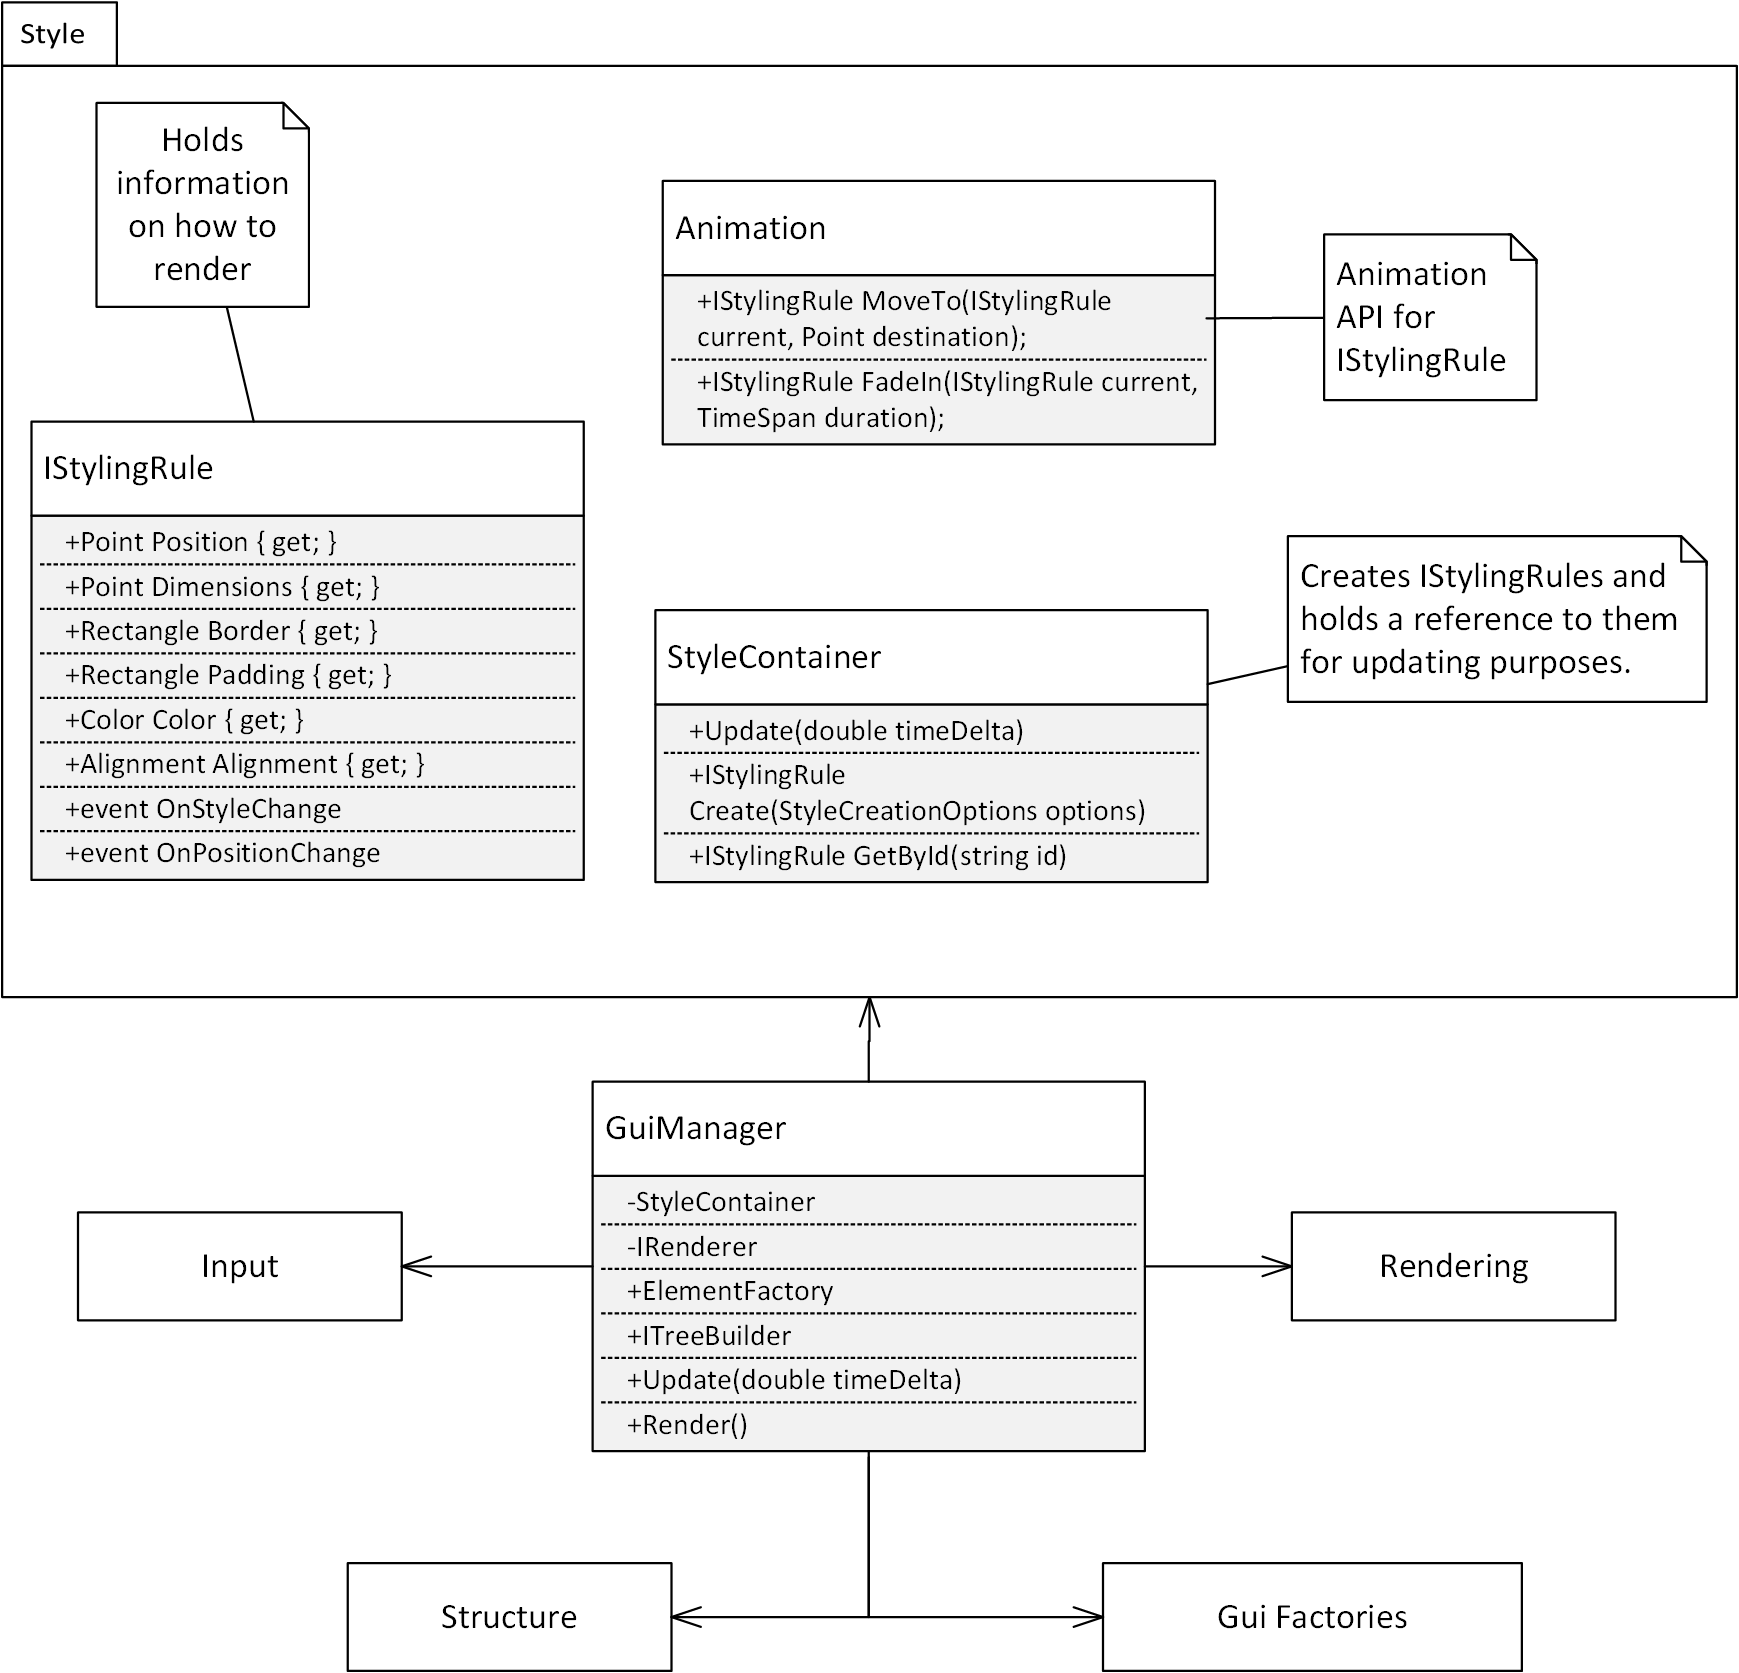
\includegraphics[width=165mm]{Images/gui_system}
		\caption{UI System UML}
		\label{fig:ui_system}
	\end{figure}	
	
\newpage
\subsection{Τρόπος χρήσης}
Η σειρά προετοιμασίας διαμόρφωσης και παρουσίασης του UI φαίνεται στο διάγραμμα \ref{fig:ui_usage}.

\begin{figure}[h!]
	\centering
	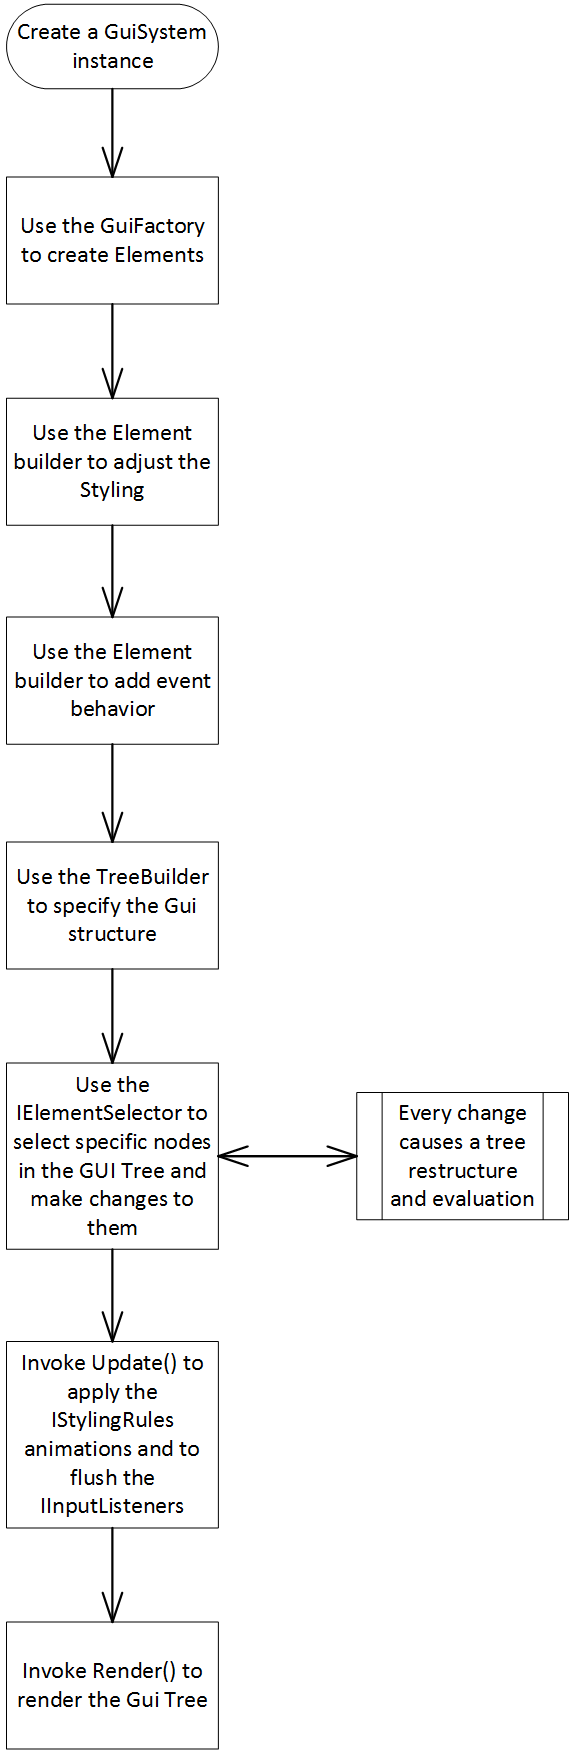
\includegraphics[width=130mm]{Images/gui_usage}
	\caption{UI Usage Diagram}
	\label{fig:ui_usage}
\end{figure}
\newpage
\section{Διαχείριση πόρων}
Τα παιχνίδια απαρτίζονται από πολλα είδη δεδομένων, είτε αυτά είναι τρισδιάστατα μοντελα, είτε είναι textures είτε αρχεία ήχου κλπ. Η μηχανή πρέπει να είναι σε θέση να φορτώνει στη μνήμη και να αφαιρεί αυτά τα δεδομένα δυναμικά. Χρειάζεται λοιπόν κάποιου είδους asset / resource manager, ο οποίος χειρίζεται το σύστημα αρχείων του λειτουργικού. Ο asset manager πρέπει να προσαρμόζεται ανάλογα με το λειτουργικό στο οποίο τρέχει και να λαμβάνει υπόψη τις ιδιαιτερότητες των διάφορων συστημάτων αρχείων. Πρέπει να υποστηρίζεται το ασύγχρονο φόρτωμα δεδομένων, για να μην μπλοκάρεται η ροή του παιχνιδιού.

Ο διαχειριστής πόρων (resource manager) απαρτίζεται από δύο μέρη. Το πρώτο χειρίζεται εργαλεία τα οποία χειρίζονται assets και τα μεταφράζουν σε μια μορφή η οποία είναι επεξεργάσιμη από τη μηχανή. Το δεύτερο διαχειρίζεται τα assets, φροντίζει να είναι διαθέσιμα όταν χρειάζονται  και όταν δεν θα ξαναχρησιμοποιηθούν φροντίζει να αφαιρέσει από τη μνήμη.
Τα περισσότερα assets δεν φορτώνονται στη μνήμη με την κανονική τους μορφή. Τα assets περνούν από κάποιο conditioning pipeline για να μετασχηματιστούν σε ένα format το οποίο μπορεί να επεξεργαστεί η μηχανή. Δεν είναι αρκετό απλά ένα μοντέλο, η μηχανή πρέπει να ξέρει για τι προορίζεται. Περιέχουν metadata το οποίο περιγράφει το πως η μηχανή θα χειριστεί το συγκεκριμένο asset. 
Χρειάζεται μια resource database η οποία ξέρει πως να χειρίζεται διάφορα είδη assets σε μια μορφή την οποία η μηχανή καταλαβαίνει. Μπορεί απλά το κάθε asset να περιέχει μαζί του κάποιο αρχείο xml το οποίο εξηγεί τι θα κάνει η μηχανή μαζί του. Επίσης είναι χρήσιμο να υποστηρίζει  versioning. Η βάση μπορεί να είναι είτε SQL είτε απλά ένα b-tree με buffer blocks και δυνατότητα προσπέλασής του. 

\paragraph{Σχεδιασμός Resource Pipeline}
\begin{itemize}
\item Granular resoures:  resources τα οποία συνδέονται με τις οντότητες στο παιχνίδι. 
\item Συνδεση με κώδικα: μπορεί εύκολα να γίνει η σύνδεση των δεδομένων με τον πηγαίο κώδικα
\item Ευκόλo export δεδομένων σε διάφορα formats.
\item Συμβατότητα με άλλα formats ή δυνατότητα μετατροπής τους σε format το οποίο είναι συμβατό με τη μηχανή.
\item Εύκολο build, αφού η μηχανή αναλαμβάνει τις εξαρτήσεις μεταξύ δεδομένων και κώδικα.
\end{itemize}

\subsection{Ευθύνες του offline resource manager}
\begin{itemize}
\item Exporters η δυνατότητα μετατροπής native format σε format το οποίο μπορεί να τροποποιηθεί από τη μηχανή.
\item Resource Compilers κατά το export χρειάζεται να γίνει κάποιου είδους καμουφλάρισμα των δεδομένων ώστε να συμβαδίζουν με την μηχανή.
\item Resource Linkers πολλές φορές περισσότερα από ένα αρχεία χρειάζονται να συνδεθούν για να δημιουργηθεί ένα χρήσιμο πακέτο. Η είναι υπεύθυνη στο να βρίσκει εξαρτήσεις και να ενώνει κομμάτια ώστε να δημιουργεί πακέτα έτοιμα χρησιμοποιηθούν.
\end{itemize}

\subsection{Ευθύνες του Runtime- Resource Manager}
\begin{itemize}
\item Εξασφαλίζει ότι στη μνήμη υπάρχουν μόνο μοναδικά resources και περισσότερα από ένα του ίδιου τύπου.
\item Διαχειρίζεται το πόσο χρόνο είναι διαθέσημα στη μνήμη
Φορτώνει και ξεφορτώνει απο τη μνήμη
\item Χειρίζεται composite resources δηλαδή resource το οποίο αποτελείται από περισσότερες από μία. Ένα τρισδιάστατο μοντέλο για παράδειγμα, αποτελείται από ένα mesh, materials, textures, skeletal animations κλπ
\item Διαχειρίζεται την ακεραιότητα των αναφορών, δηλαδή λαμβάνει υπόψη τις υποεξαρτίσεις και τις αλληλοεξαρτίζεις και φροντίζει να μην υπάρχουν προβλήματα.
\item Διαχειριση μνήμης.
\item Επιστρέπει την τροποποίηση των δεδομένων αφού φορτωθούν στη μνήμη
\item Προσφέρει τη δυνατότητα ασύγχρονης φόρτωσης για παραλληλισμό ενεργειών.
\end{itemize}

\paragraph{Οργάνωση αρχείων και καταλόγων}
Συνήθως γίνεται δενδροειδής οργάνωση για τα resources.  Πολλές φορές για σκοπούς επίδοσης, πολλά αρχεία είναι συμπιεσμένα σε ένα για να γινέται πιο γρήγορη προσπέλαση. Μια μηχανή μπορεί να χρησιμοποιήσει ήδη υπάρχων formats ή κάποιο προσαρμοσμένο για τις ανάγκες της μηχανής. 

\paragraph{Τεχνικές διαχείρισης resources στη μνήμη}
Μια συνηθισμένη τεχνική είναι η οργάνωση σε δομή δεδομένων hashtable με κλειδιά και τιμές, όπου κλειδί είναι το μοναδικό χαρακτηριστικό, ένα GUID ή η διαδρομή του αρχείου στο δίσκο. (flyweight pattern). Όταν το παιχνίδι χρειάζεται κάποιο resource, η μηχανή ελέγχει αν υπάρχει το κλειδί. Αν υπάρχει τό επιστρέφει και αν όχι τότε φορτωνεί στο hashtable.

\paragraph{Διαχείριση του κύκλου ζωής στη μνήμη}
\begin{itemize}
\item Global resources: κάποια resources φορτώνονται στην αρχή του παιχνιδιού και χρειάζονται συνέχεια.
\item Level resources: άλλα χρειάζονται στο scope συγκεκριμένου level-layout
\item Short-living resources: κάποια χρειάζονται για ένα συγκεκριμένο σκοπό κατα τι διάρκεια π.χ. μια σκηνή η οποία εμφανίζεται μια φορά κατα τη διάρκεια ενός level.
\item Live streamed resources: αρχεία μουσική και ηχητικών εφέ τα οποία διαβάζονται από το δίσκο δυναμικά και φορτώνονται σε chunks.
\end{itemize}

\paragraph{Τεχνκές διαχείρισης κύκλου ζωής}
Υπάρχουν διάφορες τεχνικές για τη διαχείρηση του κύκλου ζωής των resources. Μια καλή τεχνική είναι να φυλάονται τα references στα αντικείμενα κάθε φορά που γίνεται προσπέλαση στη μνήμη π.χ. στην αρχή κάθε level.
Μετράται πόσες φορές ζητήθηκε συγκεριμένο resource.  
Βημα 1: Βρίσκουμε όλα τα resources που χρειάζονται για τη συγκεκριμένη σκηνή και αυξάνουμε τον μετρητή τους κατά 1. Αφαιρούμε στα υπόλοιπα 1.
Βήμα 2: Σε όσα ο μετρητής έγινε 1, τα φορτώνουμε στη μνήμη και σε όσα έγινε 0 τα αφαιρούμε από τη μνήμη.

\paragraph{Αρχιτεκτονική του Runtime Resource Manager}
Η αρχιτεκτονική του runtime resource manager παρουσιάζεται στο UML διάγραμμα \ref{fig:runtime_resource_uml}
\begin{figure}[h!]
	\centering
	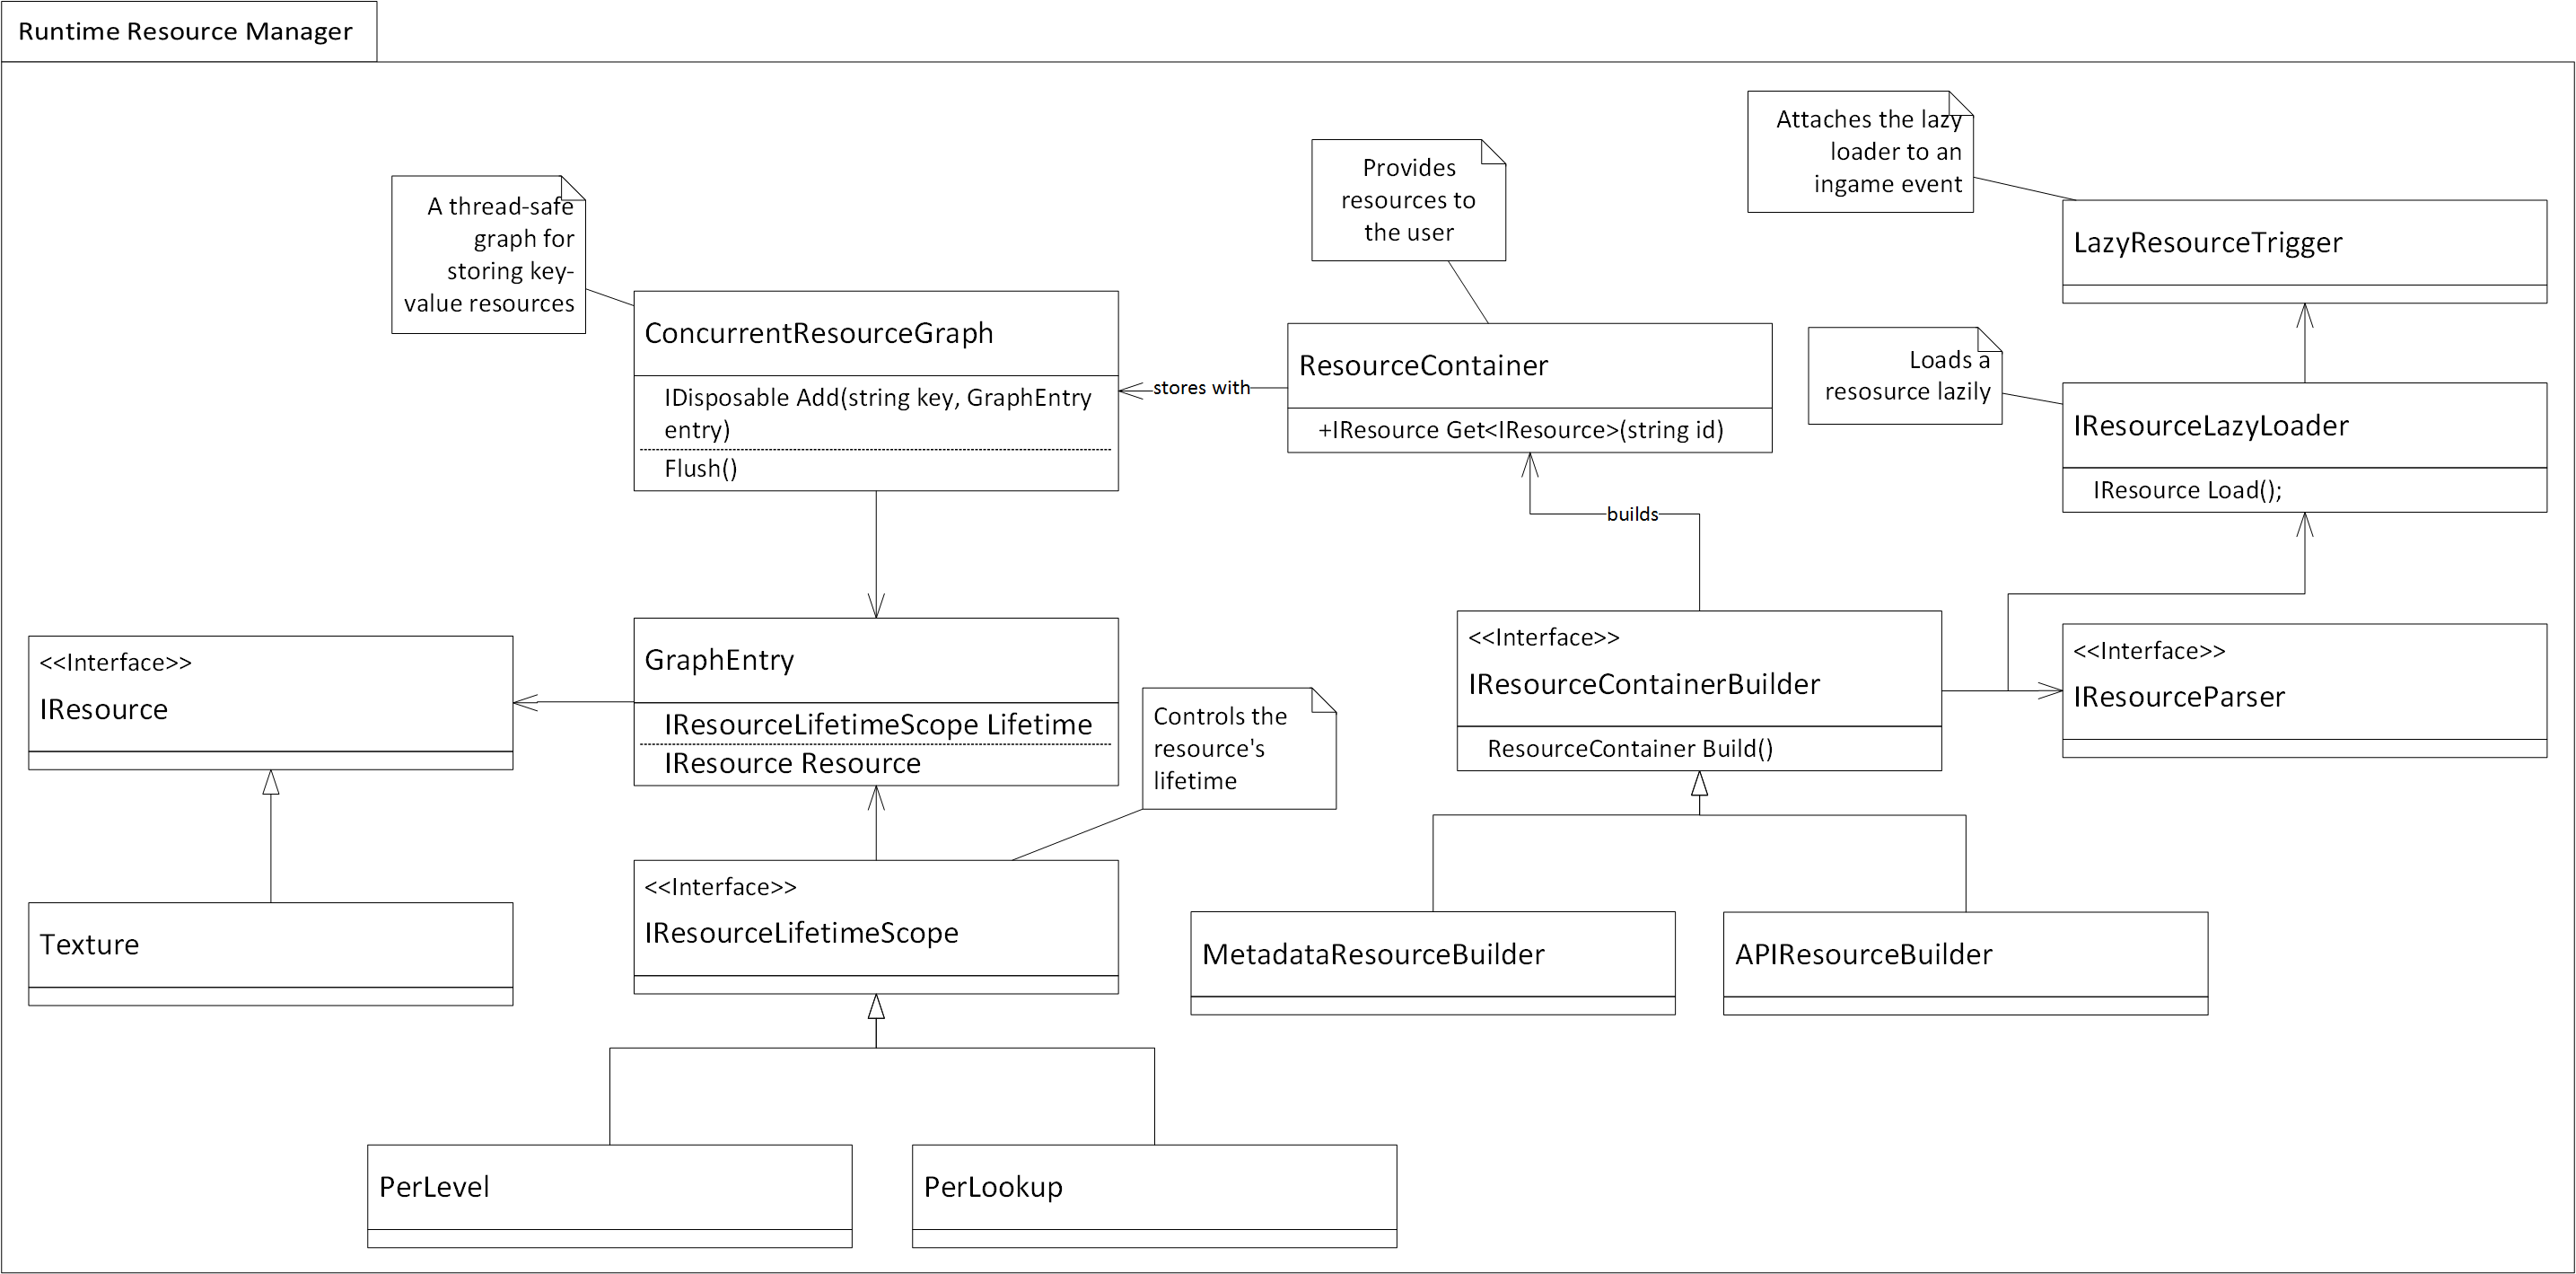
\includegraphics[width=165mm]{Images/runtime_resource_manager}
	\caption{Runtime Resource UML}
	\label{fig:runtime_resource_uml}
\end{figure}

\section{Τεχνητή νοημοσύνη}
Η τεχνητή νοημοσύνη χρησιμοποιείται για να παράγει ευφυείς συμπεριφορές κυρίως χαρακτήρες εκτός του παίχτη (NPCS). Οι αλγόριθμοι της τεχνικής νοημοσύνης προσπαθούν να προσομοιώσουν την ανθρώπινη συμπεριφορά και βασίζονται σσε τεχνικές από θεωρία ελέγχου, ρομποτική και γενικά της πληροφορικής. Στα ηλεκτρονικά παιχνίδια η νοημοσύνη συμβάλει στο πιο ρεαλιστικό gameplay μέσα στους περιορισμούς του περιβάλλοντος. Η προσέγγιση είναι εντελός διαφορετική από την τεχνητή νοημοσύνη σε άλλα πεδία, γιατί οι ικανότητες του υπολογιστή πρέπει να είναι ήπιες ώσστε να δώσει σε ανθρώπινους παίκτες μια αίσθηση δικαιοσύνης και ικανοποίησης.
 
\subsection{Δέντρα συμπεριφoρών}	
To δέντρο συμπεριφορτών (behavior tree) είναι ένα δέντρο με ιεραρχικά συνδεδεμένους κόμβους για έλεγχο της ροής της διαδικασίας λήψης αποφάσεων μιας οντότητας με νοημοσσύνη. Στα φύλλα του δέντρου βρίσκονται οι εντολές και η συμπεριφορά της οντότητας. Τα κλαδιά τα δημιουργούν διάφοροι τύποι κόμβων οι οποίοι περιέχουν εντολές και περιορισμούς για τη διάβαση του δέντρου.

Η βασική οντότητα του δέντρου είναι ο κόμβος. Ο κάθε κόμβος αξιολογείται σε κάθε βήμα διάβασης του δέντρου και επιστρέφει την κατάστασή του:
\begin{itemize}
	\item Success: Ο κόμβος αξιολογήθηκε με επιτυχία
	\item Failure: Ο κόμβος αξιολογήθηκε με αποτυχία
	\item Running: Ακόμη να τελειώσει η αξιολόγηση του κόμβου.
\end{itemize}

Η διάβαση του δέντρου προχωράει ανάλογα με την κατάσταση του προηγούμενου κόμβου. Οι κόμβοι αξιολόγησης λειτουργούν σαν λογικές πύλες.

\begin{itemize}
	\item Sequence: Προσομοιώνει την πύλη AND, για να αξιολογηθεί ο κόμβος κλαδί με επιτυχία, πρέπει όλοι οι κόμβοι του κλαδιού να αξιολογηθούν επιτυχώς.
	\item Selector: Προσομοιώνει την πύλη ΟR. Η αξιολόγηση του κλαδιού θεωρείται επιτυχημένη στην πρώτη αξιολόγηση ενός δέντρου με επιτυχία.
	\item Random Selector: Ίδια συμπεριφορά με τον selector, απλά η αξιολόγηση των κόμβων γίνεται με τυχαία σειρά.
	\item Random Sequence: Ίδια συμπεριφορά με το sequence, απλά η αξιολόγηση των κόμβων γίνεται με τυχαία σειρά.
\end{itemize}
	
H συμπεριφορά και αξιολόγηση των κόμβων μπορεί να μεταβληθεί χρησιμοποιώντας το decorator pattern.

\begin{itemize}
	\item Inverter: Ο κόμβος ο οποίος ειναι decorated από τον inverter, επιστρέφει το αντίστροφο αποτέλεσμα κατά την αξιολόγηση.
	\item Repeat Until Success: O κόμβος αξιολογείται ως Running εφόσων αξιολογηθεί με αποτυχία. 
	\item Repeater: Η αξιολόγηση του κόμβου επαναλαμβάνεται ανάλογα με το προκαθορισμένο αριθμό επαναλήψεων
	\item Max Time: Η αξιολόγηση γίνεται μέσα σε στα πλαίσια χρονικού διαστήματος.
\end{itemize}

Τα φύλλα του δέντρου καθορίζουν την πραγματική συμπεριφορά της νοημοσύνης. Τα φύλλα μπορούν να είναι:

\begin{itemize}
	\item Ερωτήσεις. Υπάρχει το συγκεκριμένο αντικείμενο στο χάρτη;
	\item Συμπεριφορά. Προχώρα μπροστά.
\end{itemize}

Στο mind map \ref{fig:behavior_trees_mind_map} παρουσιάζονται οι σχέσεις και οι τύποι των κόμβων.
\begin{figure}[h!]
	\centering
	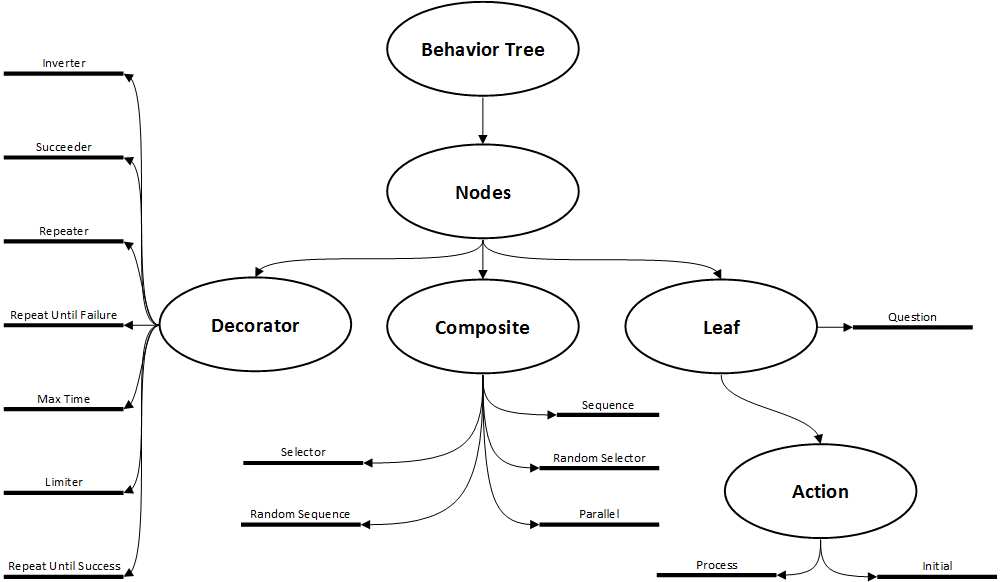
\includegraphics[width=165mm]{Images/behavior_trees}
	\caption{Behavior Trees}
	\label{fig:behavior_trees_mind_map}
\end{figure}
	
\paragraph{API}
Το API του gem engine παρέχει fluent tree builder για εύκολη δημιουργία δέντρων στη μνήμη με κώδικα και tree visualizer για απόδοση του δέντρου στην οθόνη με αξιολόγηση και ενημέρωση πραγματικού χρόνου για αποσφαλμάτωση. Στο παρακάτω παράδειγμα θα γινει μοντελοποίηση της συμπεριφοράς ενώς χαρακτήρα ο οποίος προσπαθεί να βρει την έξοδο σε ένα λαβύρινθο με εχθρούς.

	\lstset
	{
		style=sharpc, 
		caption={Behavior Tree Builder}
	}
	\begin{lstlisting}	
 behaviorBuilder
 .Selector(name: "Move to end")
	 .Decorate(For.RepeatUntilFailure)
		 .Sequence(name: "try walk")
			 .Question(CheckNextTile, name: "next tile empty?")
			 .Behavior(MoveOneTile, name: "go 1 step forward")
	 .Sequence("key obstacle")
			 .Question(CheckTileForKey, name: "found key?")
			 .Selector("handle key")
	 .End
	 .Sequence
	 .DecorateFor(Decorator.AlwaysSuccess)
		 .Behavior(RunAway)
	 .End
 .End
 .Tree;
	\end{lstlisting}


\subsection{Finite State Machines}	
 Finite state machine είναι μια αφηρημένη μηχανή η οποία μπορεί να βρίσκεται σε μία από ένα πεπερασμένο αριθμό καταστάσεων και με την επέλευση κάποιου γεγονότος μπορεί να αλλάξει από μια κατάσταση σε άλλη. 
 Κατάσταση (state) είναι η περιγραφή της κατάστασης στην οποία βρίσκεται το σύστημα.
 Γεγονός (event) δράση η οποία οδηγεί σε αλλαγή κατάστασης.
 Transition (μετάβαση) είναι ένα σύνολο δράσεων που πρέπει να εκτελεστούν όταν πληρείται μια προϋπόθεση ή όταν συμβεί ένα γεγονός. Στο UML \ref{fig:state_machine_uml} παρουσιάζονται οι σχέσεις μεταξύ των οντοτήτων του finite state machine.
 
\begin{figure}[h!]
	\centering
	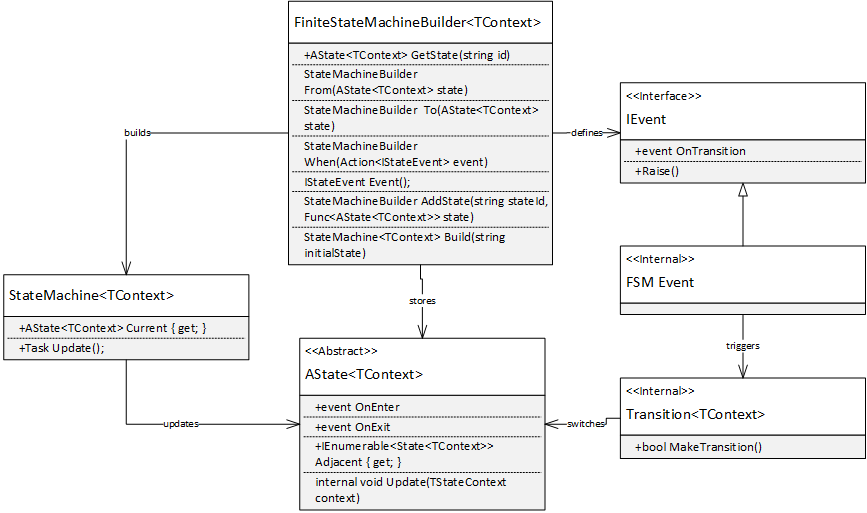
\includegraphics[width=165mm]{Images/state_machine_uml}
	\caption{State Machine UML}
	\label{fig:state_machine_uml}
\end{figure}	

Στο παράδειγμα \ref{fig:state_machine_example} μοντελοποιούνται οι καταστάσεις και τα γεγονότα τα οποία οδηγούν σε αλλαγή κατάστασης ενός χαρακτήρα με νοημοσύνη. Ο χαρακτήρας αυτός περιπλανιέται τυχαία, όταν συναντήσει αντικείμενο το μαζεύει και όταν συναντήσει εχθρό τον πολεμά. Αν ο εχθρός είναι πιο δυνατός, τότε αποφεύγει την μάχη φεύγοντας.
\begin{figure}[h!]
	\centering
	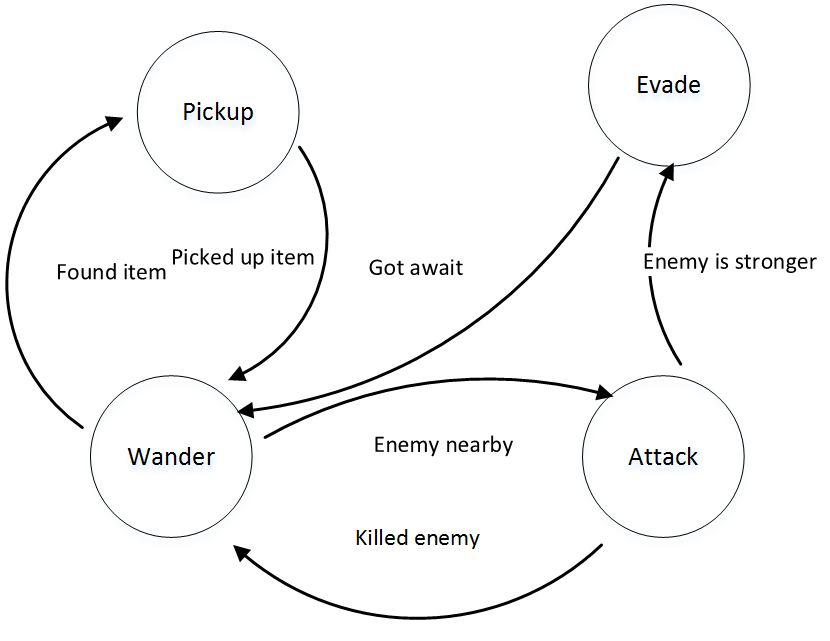
\includegraphics[width=100mm]{Images/ingame_fsm_example}
	\caption{State Machine Example}
	\label{fig:state_machine_example}
\end{figure}

H σύνδεση του finite state machine γίνεται μέσω του builder. Στον builder γίνεται καταχώρηση τον καταστάσεων μέσω μιας μεθόδου-factory και δημιουργία αυτοενεργοποιημένων συμβάντων ή συμβάντων τα οποία ενεργοποιούνται από τον χρήστη τα οποία οδηγούν σε αλλαγή κατάστασης. Μετά γίνεται το χτίσημο του FSM και η ενημέρωση του με βάση το γενικότερο πλαίσιο.

\newpage
\lstset
{
	style=sharpc, 
	caption={State machine}
}
\begin{lstlisting}	
fsmBuilder
.AddState("PickUp",() => new PickupState())
.AddState("Wander",() => new WanderState())
//with lifetime
.AddState("Attack",() => ioc.Resolve<AttackState>())
.AddState("Evade",() => new EvadeState())	
		
var attackEvent = fsmBuilder
.From("Wander")
.To("Pickup")
.When(context=> context.FoundItem) //auto triggered
	
var attackEvent = fsmBuilder
.From("Wander")
.To("Attack")
.Event() //manually triggered
	 	
world.OnCollision += (sender,args)=>
{
    if(args.CollidedType is Enemy)
	    attackEvent.Trigger();
}
	 
//emitted	 
var playerBehaviorFsm = fsmBuilder.Build("Active);
await playerBehaviorFsm.Update(playerContext);
	
\end{lstlisting}
	
		\chapter{Διαδικτύωση}
		Διαδικτύωση στα ηλεκτρονικά παιχνίδια έχουμε όταν περισσότεροι από ένας παίχτες σε διαφορετικές πλατφόρμες ή υπολογιστές, μοιράζονται και αλληλεπιδρούν στο ίδιο εικονικό περιβάλλον. 
		
		\section{Το πρόβλημα}
		\subsection{Περιγραφή του προβλήματος}
		Διάφοροι παίχτες σε διάφορα σημεία του πλανήτη θέλουν να μοιραστούν ένα εικονικό περιβάλλον σε πραγματικό χρόνο με σκοπό την συνεργασία ή την αντιπαλότητα. O κόσμος είναι ένα υπερσύνολο του offline κόσμου με επιπλέων στοιχεία κοινωνικοποίησης όπως η επικοινωνία μέσω μηνυμάτων ή φωνής.
		
		\subsection{Κατανόηση του προβλήματος}
		
		Ένας εικονικός κόσμος, περιλαμβάνει πολλές οντότητες οι  οποίες αλληλεπιδρούν μεταξύ τους μέσω των μηχανισμών, νόμων και κανόνων που διέπουν τον κόσμο. Παράδειγμα μηχανισμού είναι η προσομοίωση του φυσικού κόσμου, όπου οι οντότητες αναποκρίνονται σε νόμους της φυσικής.
		
	    Κατά την ενημέρωση του κόσμου, ο προσομοιωτής χρησιμοποιώντας  τους νόμους, τους κανόνες και τους μηχανισμούς που διέπουν τον κόσμο, παίρνει ως είσοδο τις οντότητες, τα ειδικά βάρη των ιδιοτήτων τους, την απόλυτη θέση τους στο σύστημα συντεταγμένων του κόσμου, και το χρονικό διάστημα της προσομοίωσης και αναλύει την προσομοίωση. Η ανάλυση της προσομοίωσης για να είναι επιτρεπτά ακριβής πρέπει να γίνεται περίπου 80-100 φορές το δευτερόλεπτο. [αναφορά σε πηγή]
		
		Στο τέλος της προσομοίωσης, η μηχανή γραφικών αποτυπώνει τον κόσμο στις εξόδους με αναφορές σε στατικά assets, σε αλγόριθμους παραγωγής δυναμικών assets για την αναπαράσταση του κόσμου.
	
		\subsection{Εξαγωγή απαιτήσεων}	
		Με βάση το πρόβλημα καταλήγουμε στο παρακάτω διάγραμμα ακολουθίας.
		
		\begin{figure}[h]
			\centering
			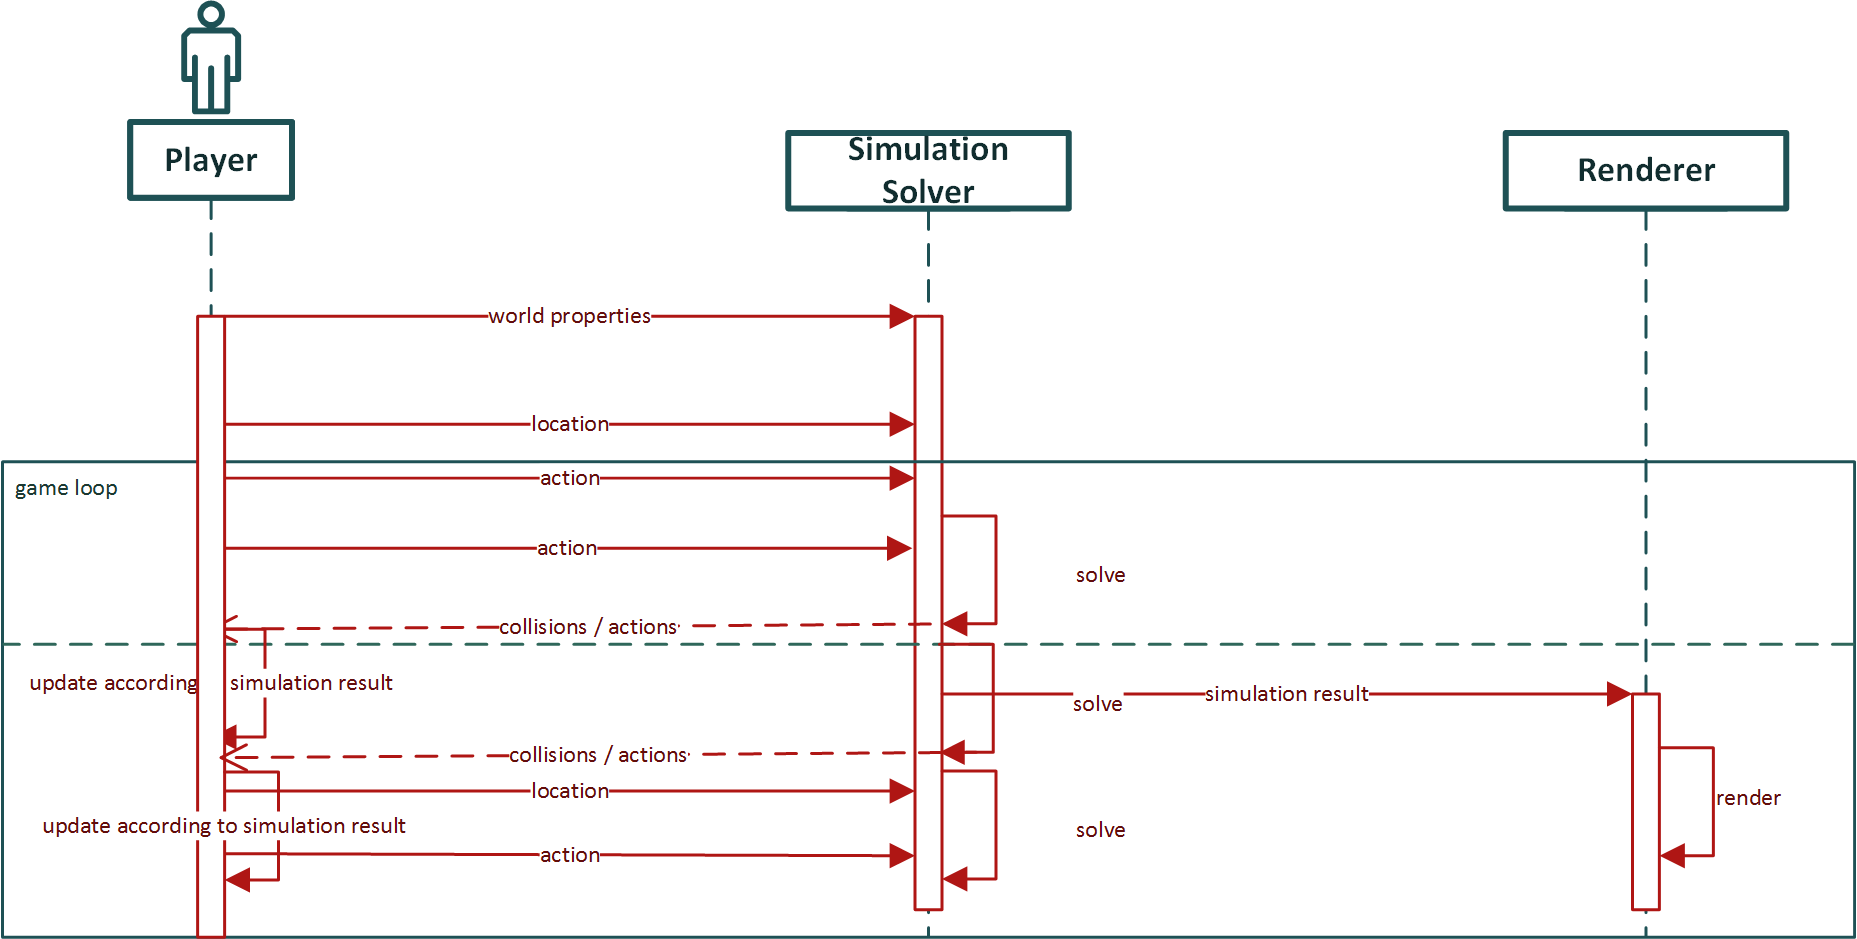
\includegraphics[width=140mm]{Images/gameloop_network_sequence}
			\caption{Network Sequence}
			\label{fig:Network Sequence}
		\end{figure}		
		
		Βλέποντας το διάγραμμα καταλαβαίνουμε ότι σε η διαδικασία rendering περιλαμβάνει στατικά στοιχεία και αλγόριθμους, τα οποίοι μπορούν να φορτώνονται τοπικά στον κάθε υπολογιστή, και δεν είναι απαραίτητα για την επίλυση της προσομοίωσης. Τα απαραίτητα στοιχεία για την προσομοίωση τα οποία πρέπει να μοιράζονται μεταξύ των παιχτών είναι:
		\begin{itemize}
			\item Oι ιδιότητες της οντότητας με βάση τους νόμους του κόσμου. Οι ιδιότητες αυτές δεν ενημερώνονται συχνά.
			\item Οι αλλαγές στο σύστημα συντεταγμένων και οι διάφορες ενέργειες της κατευθυνόμενης οντότητας κατά την πάροδο του χρόνου. Οι αλλαγές τοποθεσίας και ενέργειες γίνονται πολλές φορές ανά δευτερόλεπτο. Η προσομοίωση για να είναι ακριβής πρέπει να ενημερώνεται για τις διάφορες ενέργειες σε πραγματικό χρόνο.
		\end{itemize}
				
		\section{Εκπόνηση σχεδίου}	
		Η ανάγκη αποστολής πολλών μηνυμάτων ανά δευτερόλεπτο οδηγεί στη χρήση των network sockets. Τα sockets χρησιμοποιωντας ένα IP και  Port και επιτρέπουν την αποστολή και παραλαβή μηνυμάτων με βάση κάποιου πρωτόκολλου.
		
		\subsection{Επιλογή πρωτοκόλου}
		\begin{itemize}	
			\item TCP (transmission control protocol), είναι το πιο συχνά χρησιμοποιημένο πρωτόκολλο. Η διασύνδεση με TCP είναι αξιόπιστη και τα μηνύματα παραλαμβάνονται στη σειρά αποστολής. Η αξιοπιστία όμως έρχεται με ένα μικρό κόστος απόδοσης.
			\item UDP Το UDP (user diagram protocol) δεν περιλαμβάνει την αξιοπιστία και την εγγύηση της αλληλουχίας μηνυμάτων. Η απουσία λειτουργιών όμως, το κάνει το πιο γρήγορο σε αποστολή μηνυμάτων πρωτόκολλο.
			
			Η επιλογή πρωτοκόλλου γίνεται ανάλογα με το γενικότερο πλαίσιο και τη συγκεκριμένη χρήση του πακέτου αποστολής. Στην αποστολή της τοποθεσίας, το οποίο γίνεται 20φορές / δευτερόλεπτο, η αξιοπιστία δεν είναι το βασικότερο, αλλά η απόδοση. Στην αποστολή των στοιχειών του χρήστη κατά την έναρξη, ή ενώς γραπτού μηνύματος πρέπει να είναι αξιόπιστη.
		\end{itemize}

		\subsection{Επιλογή αρχιτεκτονικής δικτύου}
			Οι αρχιτεκτονικές δικτύου χωρίζονται ανάλογα με το που γίνεται η επίλυση και επεξεργασία της προσομοίωσης.  
		\begin{itemize}	
			\item Client-server model: στο οποίο ο client απλά κάνει render και το μεγαλύτερο κομμάτι της λογικής και της προσωμοίωσης τρέχει στον server. Ο server στέλνει οδηγίες στον client για το τι να κάνει render και ο client απλά υπακούει.
			\item Client on top of server model: ο client είναι και server, δηλαδή οι μηχανές που έχουν τον client έχουν και τον server.
			\item Peer-to-peer: οι μηχανές συμπεριφέρονται μερικώς ως clients και μερικώς ως servers, δηλαδή έχουν και στοιχεία λογικής και επεξεργασίας.
		\end{itemize}
			Η client-server αρχιτεκτονική εφαρμόζεται σε παιχνίδια τα οποία περιλαμβάνουν πολύ μεγάλους κόσμους και η προσομοίωση περιλαμβάνει αλληλεπιδράσεις μεταξύ πολλών οντοτήτων. Οι προσωμοιώσεις αυτές γίνονται σε εξειδικευμένες μηχανές και όχι στον προσωπικό υπολογιστή του κάθε χρήστη γιατί χρειάζονται μεγάλους υπολογιστικούς πόρους. Επίσης ο server μπορεί να λύσει race conditions και να λειτουργήσει ως "διαιτητής" μεταξύ δύο οντοτήτων οι οποίες ζητούν πρόσβαση στο ίδιο σύστημα κατά το ίδιο χρονικό διάστημα. Οι αρχιτεκτονικές στις οποίες ο client περιλαμβάνει στοιχεία επεξεργασίας του κοινόχρηστου κόσμου, είναι πιο δύσκολες στην ανάπτυξη συντήρηση γιατί δημιουργούνται race conditions στο χρονικό διάστημα αποστολής-παραλαβής μηνυμάτων που προορίζονται σε αλληλοεξαρτώμενες λειτουργίες.
			
		\section{Σχεδίαση του framework}
		Κατά το σχεδιασμό διαδικτυακών παιχνιδιών πολλά μοτίβα και στερεότυπα κώδικα επαναλαμβάνονται χωρίς να συμβάλλουν στην λογική ή μηχανισμούς. Σκοπός του framework είναι να μειώσει και να απλοποιήσει τον επαναλαμβανόμενο κώδικα και να προμηθεύσει τον χρήστη με μοτίβα και μοντέλα ούτως ώστε να εστιάσει μόνο στα απαραίτητα.
		
		\subsection{Έννοιες}
		\paragraph{Serialization}
		Σε μια αντικειμενοστραφή γλώσσα χρησιμοποιούνται κλάσεις για να μοντελοποιήσουν το πρόβλημα. Όμως τα αντικείμενα τον κλάσεων δεν μπορούν να σταλούν μέσω network socket στην αρχική τους μορφή, πρέπει να γίνει μια μετατροπή σε binary για να είναι συνεπής με το format των δεδομένων που αποστέλλονται μέσω του socket . Κατά την αποστολή έχουμε το serialization τον αντικείμενων, και κατά την παραλαβή το deserialization του πακέτου στο αντικείμενο που αντιπροσωπεύει.
		\subsection{Τύποι μηνυμάτων}
		Οι διάφοροι τύποι μηνυμάτων χρησιμοποιούνται για να ξεχωρίσουν την κατάσταση στην οποία βρίσκεται ο client ή ο server.
			\begin{itemize}
				\item Αλλαγή κατάστασης
				\begin{itemize}
					\item Connecting
					\item Connected
					\item Disconnecting
					\item Disconnected
				\end{itemize}
				\item Data
				\item ErrorMessage
				\item WarningMessage
				\item VerboseMessage
				\item ConnectionApproval
				\item DiscoveryRequest
				\item DiscoveryResponse
			\end{itemize}
		Οι τύποι μηνυμάτων μπορούν να μοντελοποιηθούν ως ένα enum και να προστεθεί η πληροφορία τους στο πρώτο byte του serialized μηνύματος. Το πρώτο byte του παραληφθέντα μηνύματος περιλαμβάνει τον τύπο του μηνύματος.
		
		\subsection{NetworkManager}
		Ο network manager είναι υπεύθυνος για την διαχείριση των sockets, την αποστολή / παραλαβή μηνυμάτων, ενθυλακώνει λειτουργιες για την διαδικτύωση και είναι ο πηρύνας του framework και επεκτίνεται από τον client, server οι οποίοι προσθέτουν λειτουργίες.
			
		\section{Υλοποίηση}	
		\subsection{Τρόπος χρήσης}
		Η διαδικασία χρήσης πρέπει να είναι εξορθολογιστική και ξεκάθαρη για εύκολη και γρήγορη ανάπτυξη και περιοριστική για αποφυγή bugs και προβληματων.
		\begin{figure}
			\centering
			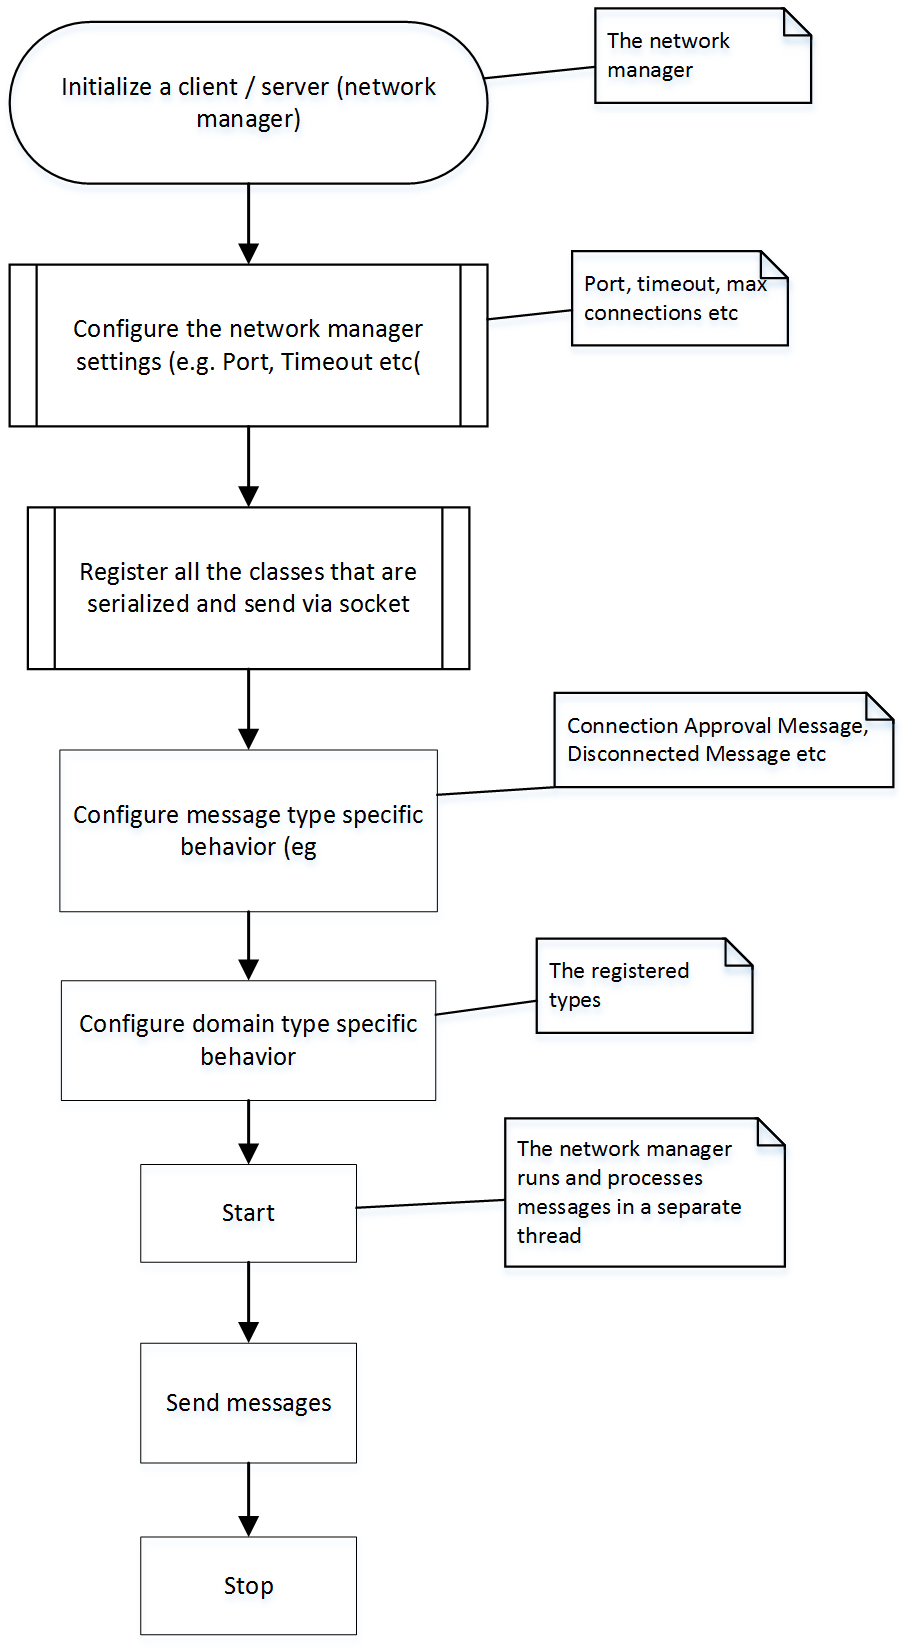
\includegraphics[width=100mm]{Images/network_usage_diagram}
			\caption{Network Usage Diagram}
			\label{fig:Network Usage_Diagram}
		\end{figure}	
					
		\subsection{Αρχιτεκτονική}	
		Η αρχιτεκτονική στηρίζεται στην ανταλλαγή μηνυμάτων-κλάσεων και χωρίζεται στα παρακάτω επίπεδα.
			\begin{itemize}
				\item {Packages} Χειρίζεται το serialization, αναλύει τα εισερχόμενα μηνύματα και χειρίζεται τις ανακατευθύνσεις του εκτελούμενου κώδικα κατά την παραλαβή μηνυμάτων. 
				\item {Networking} Διαχειρίζεται τις συνδεσεις των χρηστών, τα sockets και ο,τι έχει να κάνει με διασύνδεση.
				\item {Auditing} Αφαιρετικό επίπεδο για logging. Ο χρήστης μπορεί να ενσωματώσει τη δική του λογική παρακολούθησης μηνυμάτων.
				\item{Infrastructure} Το επίπεδο αυτό περιέχει επαναχρησιμοποιήσημο κώδικα των πακέτων όπως το ConcurrentRepository, για thread-safe αποθήκευση κλειδιών και τιμών, και το ParallelBufferBlock το οποίο εκτελεί κώδικα σε buffer άλλου thread για ασύγχρονη επεξεργασία.
			\end{itemize}
			
			\subsection{Packages Module}	 
			Το serialization των μηνυμάτων πρέπει να είναι ντερερμενιστικό ώστε να αναγνωρίζεται ο τύπος του μηνύματος και η κλάση την οποία αντιπροσωπεύει και ελαφρύς ώστε να μην επιβαρύνεται το network με επιπλέον δεδομένα. Ο ενσωματομένος serializer χρησιμοποιεί reflection για να αναγνωρίσει τα primitive properties της κλάσης. Για προχωριμένο serialization περίπλοκων τύπων, ο χρήστης έχει τη δυνατότητα να συμπεριλάβει τον δικό του serializer με το implementation του IPackageSerializer interface και την χωρήγηση του σημειώνοντας την κλάση με το PackageSerializerAttribute και τον τύπο του serializer.
			
			
			Κατά την προετοιμασία του network manager, o χρήστης καλείται να καταχωρίσει στο Container ποιες κλασεις θα χρησιμοποιηθούν κατά την ανταλλαγή μηνυμάτων. Οι κλάσεις που προωρίζονται για serialization σημειώνονται με κάποιο Attribute και η καταχώριση μπορεί να γίνει δυναμικά με reflection.
			Όταν τελειώσει η καταχώριση, το container χρησιμοποιώντας ένα ντετερμενιστικό αλγόριθμο ταξινομώντας με βάση το όνομα της κλάσης στο χώρο ονομάτων κτίζει ένα thread safe repository στο οποίο καταχωρείται ένα μοναδικό byte για αναγνωριστικό του κάθε τύπου και πληροφορίες για την χρήση του τύπου.
			
			Στο τέλος της καταχώρισης και της κατασκευής αλγόριθμου αντιστοίχισης αντικειμένων και λογικής, ο χρήστης μπορεί να καταχωρίσει εκτελέσημο κώδικα υπό μορφή function o οποίος εκτελείται ασύγχρονα κατά την παραλαβή κάποιου μηνύματος-κλάσης, τύπου μηνύματος, ή συμβάντος συγκεκριμένης σύνδεσης.
			
			\begin{figure}
				\centering
				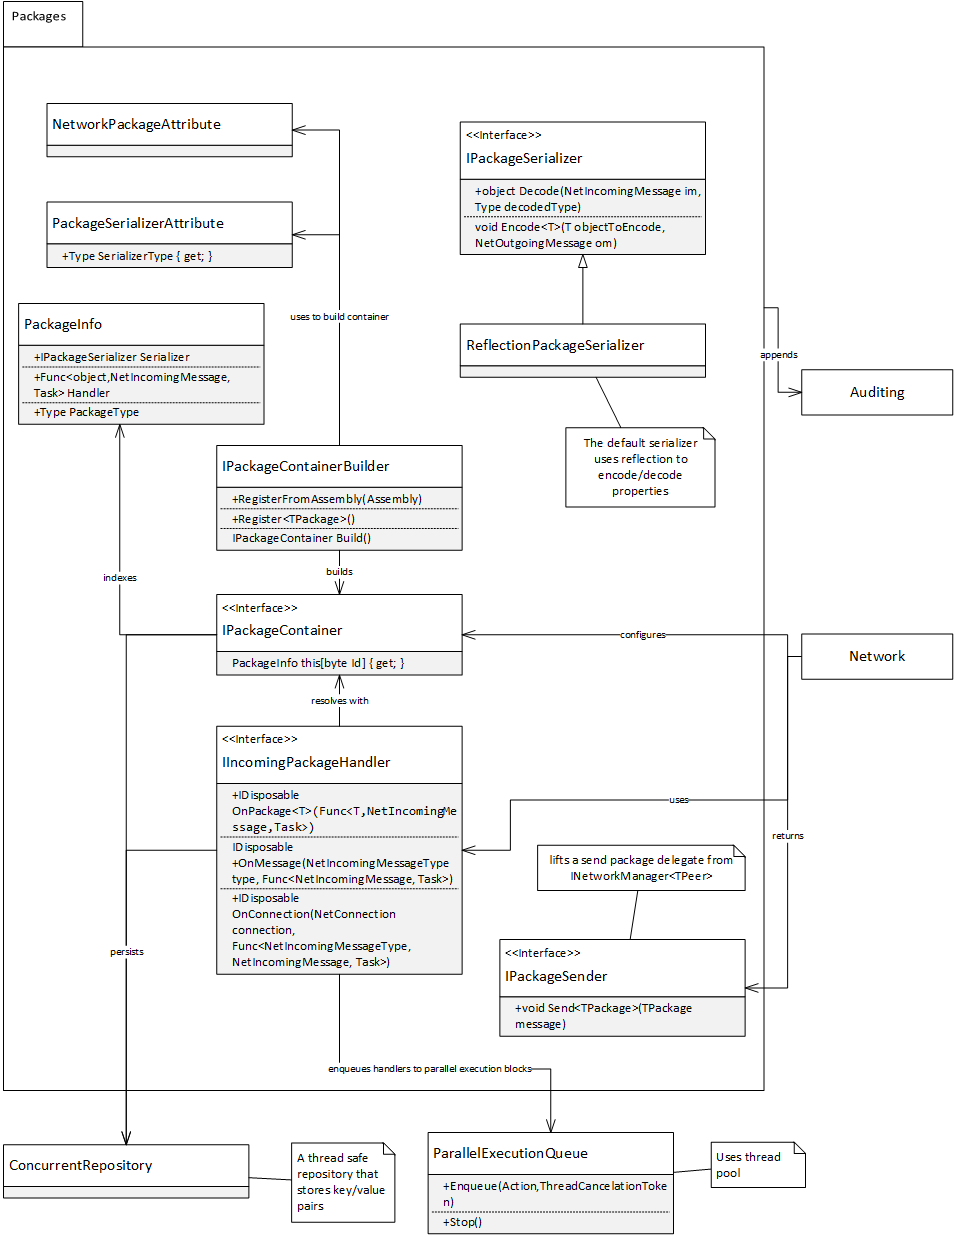
\includegraphics[width=165mm]{Images/network_architecture_packages}
				\caption{Network Packages Module}
				\label{network_packages}
			\end{figure}	
					
			\subsection{Networking Module}	 					
			
			Οι ρυθμίσεις του network manager κτίζονται από αφαιρέσεις. Η χρήση πρωτοκόλλων και τεχνικών γίνεται με άγνοια της υλοποίησης και λεπτομερειών.
			Η σχεδίαση επιτρέπει την αποστολή μηνύματος ανεξαρτήτου πρωτοκόλου, τρόπο αποστολής και παραλήπτη. Ο network manager περιλαμβάνει τεχνικές function lifting για αποστολή μηνυμάτων. Ο χρήστης μπορεί να ρυθμίσει διάφορους τρόπους αποστολής ανάλογα με το περιβάλλον χρήση, και να τους κρύψει πίσω από functions. 
						
			\begin{figure}
				\centering
				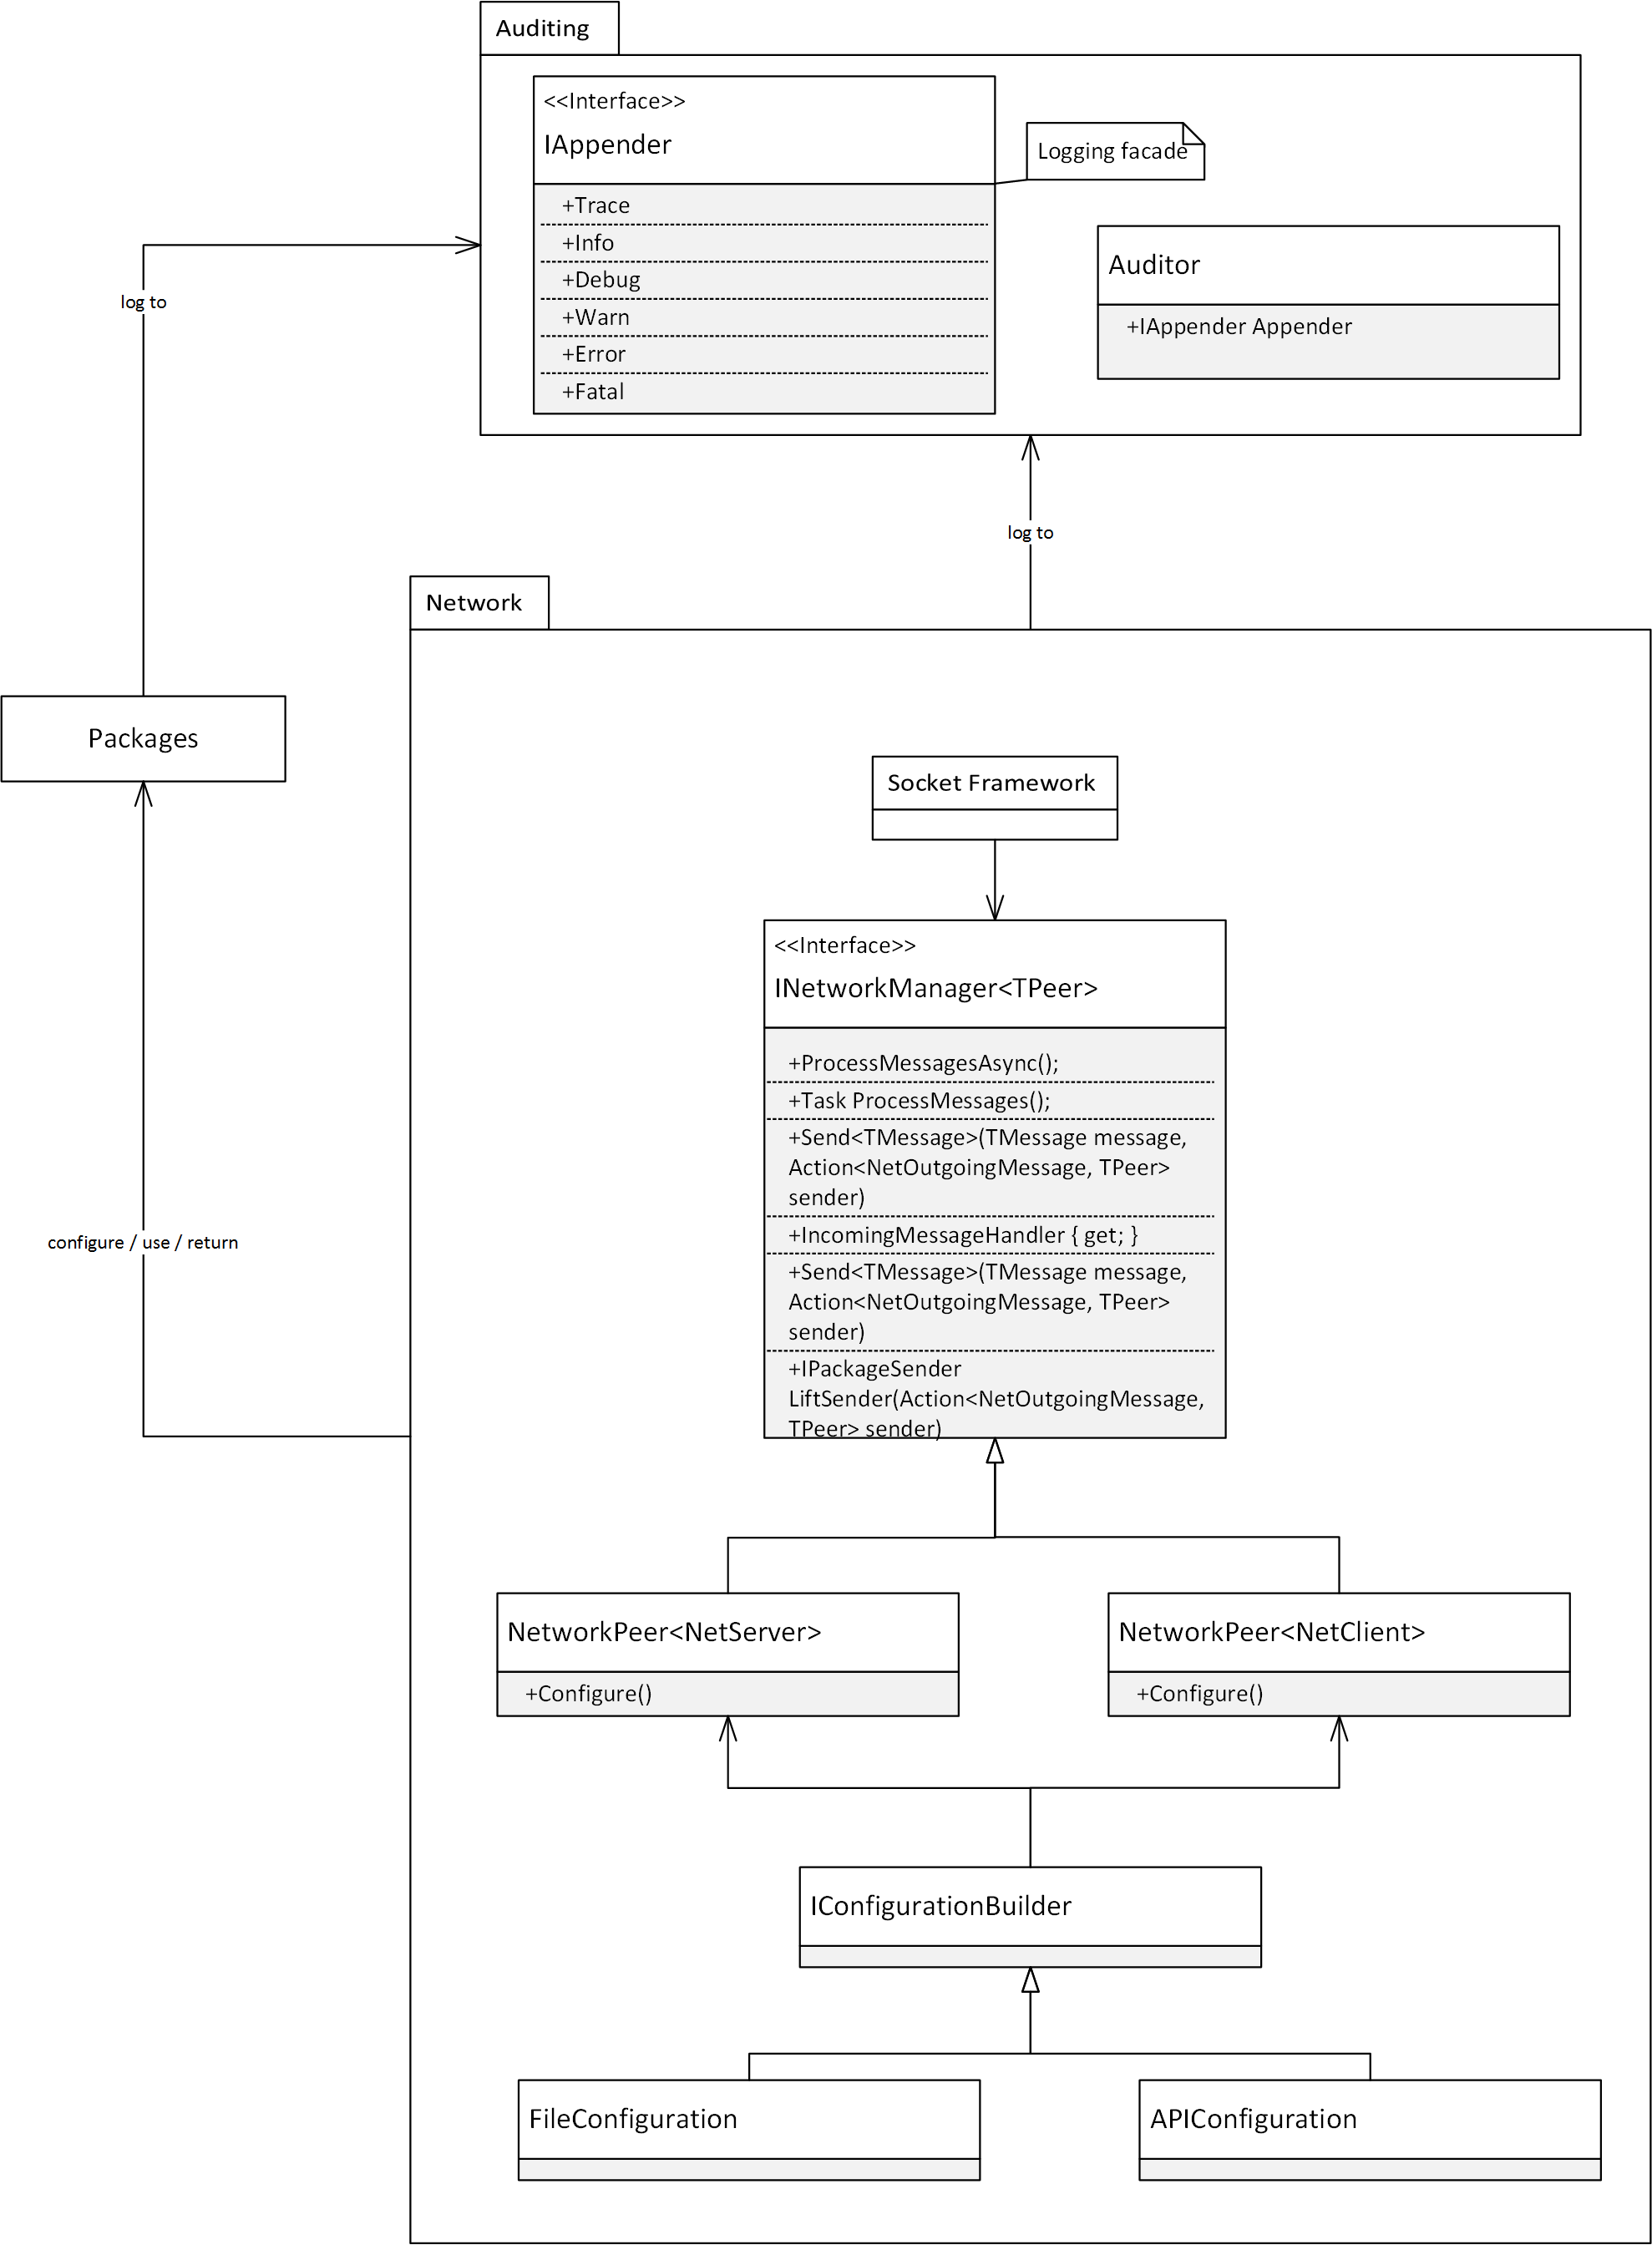
\includegraphics[width=165mm]{Images/network_architecture_networking}
				\caption{Networking Module}
				\label{networking_module}
			\end{figure}		

	\subsection{API}
	Συντομη επισκόπηση του API.
	\begin{itemize}
		\item Κλάσεις που προορίζονται για ανταλλαγή μηνυμάτων
		\lstset{style=sharpc}
		\begin{lstlisting}
[GinetPackage]
 //optional
[PackageSerializer(typeof(MyCustomSerializer))]
public class MyPackage
{
    public string Message { get; set; }
}          
		\end{lstlisting}
		\item Ρύθμιση server
		\lstset{style=sharpc}
		\begin{lstlisting}     
var server = new NetworkServer("MyServer",
builder =>
{
	//via reflection
	builder.RegisterPackages(
		Assembly.Load("Packages.Assembly.Name"));
	//or manually
	builder.RegisterPackage<MyPackage>();
}
cfg =>
{
	cfg.Port = 1234;
	cfg.ConnectionTimeout = 5.0f;
	cfg.MaxConnections = 10;
	//Additional configuration
}
//optional, logging output, default is the one supplied			 
out: new ActionAppender(Console.WriteLine) 
		\end{lstlisting}
		\item Καταγραφή κινήσεων		
		\lstset{style=sharpc}
		\begin{lstlisting}
server.IncomingMessageHandler.LogTraffic();
		\end{lstlisting}		
		\item Απάντηση κατά την παραλαβή μηνύματος
		\lstset{style=sharpc}
		\begin{lstlisting}
server.Broadcast<ChatMessage>((msg, im, om) =>
{
	server.Out.Info($"Received {msg.Message}");
	server.SendToAllExcept(om, im.SenderConnection, NetDeliveryMethod.ReliableOrdered, channel: 0);
}, 
packageTransformer: msg => 
msg.Message += "this is broadcasted");	


server.BroadcastExceptSender<ChatMessage>((sender, msg) =>
{
	server.Out.Info($"Broadcasting {msg.Message}. Received from: {sender}");
});
		\end{lstlisting} 		

		\item Κώδικας ο οποίος εκτελείται κατά την παραλαβή συγκεκριμένου τύπου μηνύματος
		\lstset{style=sharpc}
		\begin{lstlisting}
server.IncomingMessageHandler.OnMessage(
	NetIncomingMessageType.ConnectionApproval, 
	incomingMsg =>
{
	//Configure connection approval
	var parsedMsg = server
		.ReadAs<ConnectionApprovalMessage>(incomingMsg);
	if(parsedMsg.Password ==
		 "my secret and encrypted password")
	{
		incomingMsg.SenderConnection.Approve();
		incomingMsg.SenderConnection.Tag = 
			parsedMsg.Sender;
	}
	else
	{
		incomingMsg.SenderConnection.Deny();
	}
});
		\end{lstlisting}
		\item Εκτελέσιμος κώδικας κατά την παραλαβή συγκεκριμένου μηνύματος-κλάσης
		\lstset{style=sharpc}
		\begin{lstlisting}
server.IncomingMessageHandler
.OnPackage<MyPackage>((msg, sender) => 
	Console.WriteLine(
	$"{msg.Message} from {sender.SenderConnection}"));
		\end{lstlisting}	
		\item Αποστολή μηνύματος-κλάσης
		\lstset{style=sharpc}
		\begin{lstlisting}
server.Send(
	new MyPackage { Message = "Hello" },
(outgoingMessage,peer) => 
	peer.SendMessage(outgoingMessage,
		NetDeliveryMethod.ReliableOrdered);
		\end{lstlisting}		
		\item Lift αποστολής μηνύματος
		\lstset{style=sharpc}
		\begin{lstlisting}
var packageSender = client.LiftSender((msg, peer) =>
	peer.SendMessage(msg, 
		NetDeliveryMethod.ReliableOrdered));
		
packageSender.Send(new MyPackage { Message = "Hello" });	
		\end{lstlisting}	
		\item Διαγραφή handler
		\lstset{style=sharpc}
		\begin{lstlisting}	
var handlerDisposable = server.IncomingMessageHandler
	.OnPackage<MyPackage>((msg, sender) => {}));
		
handlerDisposable.Dispose();	
		\end{lstlisting}		
		\item Η ρύθμιση και το API του client είναι πανομοιότυπo με του server. Στη θέση του \textit{NetworkServer} χρησιμοποιείται ο \textit{NetworkClient} όπου και τα δύο υλοποιούν τον \textit{NetworkManager<TPeer> where TPeer:NetPeer}		
	\end{itemize}
	
	\section{Testing}
	Μια καλή αρχιτεκονική υποστηρίζεται από την ευκολία της δοκιμαστικότητας ανά μονάδα (unit testability). Το framework χρησιμοποιεί functional τεχνικές, οι οποίες εύκολα μπορούν να αντικατασταθούν με mocks. Ο χρήστης μπορεί να απομιμήσει την παραλαβή ή αποστολή πακέτων και να ενημερώνει την μονάδα επεξεργασίας μηνυμάτων από το τρέχων thread.
	
	\lstset{style=sharpc}
	\begin{lstlisting}
	
[TestMethod]
public void Incoming_Package_GetsHandled()
{
	//Arrange
	var client = new NetworkCliient(
		builder => 
			builder.Register<MyPackage>(),
		cfg=> {});
		
	var mockedHandler = 
		new Mock<Func<MyPackage,NetIncomingMessage>>();
	mockedHandler.Setup( x => 
		x(It.IsAny<MyPackage>()));
	
	client
	.IncomingMessageHandler
	.OnPackage<MyPackage>(mockedHandler);	
	
	//Act	
	client.IncomingMessageHandler.SimulateReceive(
		new MyPackage());	
	client.ProcessMessages().RunSynchronously();
	
	//Assert
	mockedHandler.Verify(x=>x(), Times.Once()));
}
	\end{lstlisting}
		
	Επίσης παρέχεται η δυνατότητα της προσομοίωσης χαμένων πακέτων, για να δοκιμαστεί πως η εφαρμογή ανταποκρίνεται σε περιβαλλον κακής διαδικτύωσης και να αναπτυχθούν τεχνικές network prediction για εξομάλυνση της κίνησης.
	
	
	\section{Ανάλυση των επιδόσεων}
	Benchmarkings here
	\begin{table}[h]
		\centering
		\caption{Network Benchmarkings}
		\begin{tabularx}{\linewidth}[h]{|XXX|}%
			\hline
			\hline
			Κίνητρα & Παραδείγματα ευρημάτων & Αριθμός μελετών\\
			\hline
			Ταύτιση με το έργο & Ξεκάθαροι στόχοι &20\\
			Καλό management & Ομαδικότητα &16\\
			Συμμετοχή υπαλλήλων & Συμμετοχή στις αποφάσεις&16\\
			Προοπτικές εξέλιξης & Προοπτικές προαγωγής&15\\
			Ποικιλία στην εργασία & Καλή χρήση ικανοτήτων& 14\\
			Αίσθηση του να ανήκεις κάπου& Υποστηρικτικές σχέσεις&14\\
			Αμοιβές και κίνητρα & Αυξημένος μισθός& 14\\
			\hline
			\hline
		\end{tabularx}
		\label{tab:network benhmarkings}
	\end{table}
	
	\section{Επεκτασιμότητα}
	Lobbies and matchmakings	
	\chapter{Διαγνωστικά και Αποσφαλμάτωση}
Η ανάπτυξη του λογισμικού πρέπει να παρακολουθείται συνεχώς. Σε λογισμικά όπως ένα παιχνίδι, η επίδοση της εφαρμογής είναι εξαιρετικά σημαντική. Για τη μετάβαση από δοκιμαστικές σε τελικές εκδόσεις, χρειάζεται συλλογή και ανάλυση διαγνωστικών επιδόσεων για διαφορετικές πλατφόρμες, επεξεργαστές και κάρτες γραφικών. Ακόμη και στις τελικές εκδόσεις όμως υπάρχει η πιθανότητα σφάλματος. \cite{richter2012clr}

\section{Logging and Tracing}
Ένα logfile είναι ένα αρχείο το οποίο περιέχει γεγονότα τα οποία συμβαίνουν κατά την εκτέλεση ενός λογισμικού. Logging ονομάζουμε τη διαδικασία καταγραφής μηνυμάτων σε ένα logfile ανάλογα με το επίπεδο σημαντικότητας. Ένα εξειδικευμένο είδος logging είναι το tracing, στο οποίο καταγράφονται πληροφορίες για την εκτέλεση του προγράμματος. Χρησιμοποιείται κυρίως κατά την αποσφαλμάτωση αλλά και για συλλογή πληροφοριών με σκοπό την βελτίωση του λογισμικού για καλύτερη εμπειρία χρήστη.

Όταν συμβεί ένα κρίσιμο σφάλμα το οποίο οδηγεί στον τερματισμό του παιχνιδιού, πρέπει να δημιουργηθεί ένα crash report και να σταλεί στους προγραμματιστές για να εντοπίσουν το σφάλμα.
Το crash report πρέπει να περιλαμβάνει:
\begin{itemize}
 \item Το στιγμιότυπο του χρόνου σε UTC.
 \item To επίπεδο στο οποίο παρουσιάστηκε το σφάλμα.
 \item Την τοποθεσία του παίχτη.
 \item Την κατάσταση του παίχτη.
 \item Τα τρέχον gameplay scripts.
 \item Exception και stack trace.
 \item Την κατάσταση κατανομής μνήμης.
 \item Στιγμιότυπο οθόνης.
\end{itemize}

\section{Time Benchmarker}
Ο time ruler προσφέρει δυναμική ανάλυση του χρόνου εκτέλεσης και των ενημερώσεων με απόδοση πραγματικού χρόνου στην οθόνη με παραμετροποιήσιμα ονόματα και χρώμα μεταξύ της έκτασης υπολογισμού του. O time ruler παίρνει στιγμιότυπα του χρόνου κατά το χρόνο εκτέλεσης και τα αποδίδει ως μέσο όρο ανά δευτερόλεπτο στην οθόνη με τη μορφή γραμμής προόδου.
Η απόδοση και τα πλαίσια υπολογισμού είναι τροποποιήσιμα και ελεγχόμενα από το σύστημα διαγνωστικών για εύκολη εναλλαγή. Στο παράδειγμα κώδικα \ref{lst:diagnosticsAPI} παρουσιάζεται ένα απλό παράδειγμα χρήσης του time ruler για ανάλυση αλγορίθμου.

\lstset
{
	style=sharpc, 
	caption={Time Ruler},
	label={lst:diagnosticsAPI}
}

\begin{lstlisting}
string aiRuler = "Enemy_AI_Pathfinding";
diagnostics.AddTimeRuler(rulerId,Color.Red);
diagnostics.TimeRuler[aiRuler].Show = true;

using(diagnostics.TimeRuler[aiRuler].Benchmarker)
{
	//benchmarking logic here
}
\end{lstlisting}

\section{Debug Drawing API}
Μία οντότητα η οποία αποδίδεται στην οθόνη περιέχει περισσότερες πληροφορίες από αυτό που δείχνει. Μια οντότητα αν συμμετέχει στη προσομοίωση φυσικής έχει ταχύτητα και μάζα, αν συμμετέχει στο σύστημα συγκρούσεων έχει κουτί σύγκρουσης το οποίο δείχνει τα όρια σύγκρουσης με άλλα αντικείμενα και πολλές άλλες πληροφορίες σχετικά με την κατάσταση στο παιχνίδι.
Το υποσύστημα των διαγνωστικών παρέχει λειτουργίες αποσφαλμάτωσης με απόδοση στην οθόνη και να είναι προσβάσιμο από τα υπόλοιπα συστήματα. Ο κώδικας αυτού του συστήματος παραλείπεται στα release builds. Αυτό επιτυγχάνεται με τη χρήση των conditionals τα οποία χρησιμοποιούν οδηγίες προεπεξεργαστή.

Το υποσύστημα προσφέρει δυνατότητες απόδοσης για τα παρακάτω:
\begin{itemize}
	\item Βασικά σχήματα
	\item Σημεία
	\item Σφαίρες
	\item Άξονες συντεταγμένων
	\item Κουτιά οριοθέτησης
	\item Formatted text
	\item Δυνατότητα εναλλαγής χρωμάτων
\end{itemize}

\section{Υποσυστήματα αποσφαλμάτωσης}
Το σύστημα αποσφαλμάτωσης και διαγνωστικών περιέχει πολλά υποσυστήματα. Μερικά από αυτά είναι τα παρακάτω:

\begin{itemize}
	\item Μενού επιλογών στο παιχνίδι με δυνατότητα εναλλαγής επιλογών και τροποποίησης τιμών.
	\item Debug camera η οποία κινείται χωρίς περιορισμούς στο χώρο.
	\item Κονσόλα η οποία εκτελεί scripts και εντολές υπό τη μορφή κειμένου παρόμοια με το Unix Shell.
	\item Assertions εντολές οι οποίες αν δεν αξιολογηθούν ως αληθές κατά το χρόνο εκτέλεσης του λογισμικού, τερματίζουν το λογισμικό με κωδικό σφάλματος.
	\item FPS Counter το οποίο αποδίδει στην οθόνη τον αριθμό τον \gls{FPS}.
	\item Δυνατότητα παύσης.
	\item Cheats.
	\item Screenshots και screen captures.
	\item Ιngame profiler και profiling blocks με αναγνώσιμα ονόματα.
	\item Ιεραρχικό Profiling.
	\item Εξαγωγή δεδομένων σε μορφή η οποία είναι εύκολα αναγνώσιμη από άνθρωπο για αποσφαλμάτωση.
	\item Στατιστικά μνήμης και ανίχνευση διαρροών.
\end{itemize}
		
	\appendix
	\printnoidxglossaries
	\printbibliography
	\lastpageinfo

\end{document}
